% SIAM Article Template
\documentclass[review,onefignum,onetabnum]{siamart190516}

% Information that is shared between the article and the supplement
% (title and author information, macros, packages, etc.) goes into
% ex_shared.tex. If there is no supplement, this file can be included
% directly.

% SIAM Shared Information Template
% This is information that is shared between the main document and any
% supplement. If no supplement is required, then this information can
% be included directly in the main document.


% Packages and macros go here
\usepackage{lipsum}
\usepackage{amsfonts}
\usepackage{graphicx}
\usepackage{epstopdf}
\usepackage{amsmath}
\usepackage{subcaption}
\usepackage{pgfplots}

%\usepackage{amsmath,amsthm}
%\usepackage[noend]{algorithmic}
%\usepackage{algorithmic}
\usepackage[algo2e, ruled, noend, linesnumbered]{algorithm2e}
%\usepackage[algo2e, ruled, vlined]{algorithm2e}
\usepackage{bm}
\ifpdf
  \DeclareGraphicsExtensions{.eps,.pdf,.png,.jpg}
\else
  \DeclareGraphicsExtensions{.eps}
\fi

\usepackage{placeins}
\usepackage{multirow}

% Add a serial/Oxford comma by default.
\newcommand{\creflastconjunction}{, and~}
\newcommand{\nor}[1]{\left\|#1\right\|}

% Used for creating new theorem and remark environments
\newsiamremark{remark}{Remark}
\newsiamremark{hypothesis}{Hypothesis}
\crefname{hypothesis}{Hypothesis}{Hypotheses}
\newsiamthm{claim}{Claim}
\newsiamthm{prop}{Proposition}
\newsiamthm{defn}{Definition}
\newsiamthm{thm}{Theorem}
\newsiamthm{cor}{Corollary}
\newsiamthm{lem}{Lemma}


\newcommand{\norm}[1]{\|#1\|}


% Sets running headers as well as PDF title and authors
\headers{Matrix-free PSF approximation}{N. Alger, T. Hartland, N. Petra, and O. Ghattas}

% Title. If the supplement option is on, then "Supplementary Material"
% is automatically inserted before the title.
\title{Matrix-free point spread function approximation of operators with locally supported non-negative integral kernels, with application to Hessians in PDE constrained inverse problems\thanks{Submitted to the editors DATE.
\funding{This research was supported by the National Science Foundation under Grant No. DMS-1840265 and CAREER-1654311.}}}

% Authors: full names plus addresses.
\author{Nick Alger\thanks{Oden Institute, The University of Texas at Austin, Austin, TX 
  (\email{nalger@oden.utexas.edu}).}
\and Tucker Hartland\thanks{Department of Applied Mathematics, University of California, Merced, Merced, CA. 
	(\email{thartland@ucmerced.edu}).}
\and Noemi Petra\thanks{Department of Applied Mathematics, University of California, Merced, Merced, CA. 
  (\email{npetra@ucmerced.edu}).}
\and Omar Ghattas\thanks{Oden Institute, The University of Texas at Austin, Austin, TX 
	(\email{omar@oden.utexas.edu}).}}

\newcommand{\Aop}{\mathcal{A}}
\newcommand{\AopPc}{\mathcal{A}_\text{pc}}
\newcommand{\AopPcMesh}{\mathcal{A}_\text{pc}^h}

\newcommand{\Aker}{\Phi}
\newcommand{\AkerPc}{\Phi_\text{pc}}
\newcommand{\AkerPcMesh}{\Phi_\text{pc}^h}

\newcommand{\AkerPcMat}{\mathbf{\Phi}_\text{pc}}

\newcommand{\Amat}{\mathbf{A}}
\newcommand{\AmatPc}{\mathbf{A}_\text{pc}}
\newcommand{\AmatPcSym}{\mathbf{A}_\text{pc}^\text{sym}}
\newcommand{\AmatPcSymPlus}{\mathbf{A}_\text{pc}^{\text{sym}+}}

\newcommand{\diraccomb}{\xi}
\newcommand{\combresponse}{\eta}
\newcommand{\weakadmconst}{C}
\newcommand{\horizinterpolant}{\theta}
\newcommand{\interpolatedvalues}{b}
\newcommand{\firstgreens}{G}
\newcommand{\secondgreens}{F}
\newcommand{\impulseresponse}{\phi}
\newcommand{\convkernel}{\varphi}
\newcommand{\febasis}{\psi}
\newcommand{\ratfct}{R}
\newcommand{\ratpole}{\omega}
\newcommand{\ratcoeff}{c}
\newcommand{\massmatrix}{\mathbf{M}}
\newcommand{\spatialvol}{V}
\newcommand{\spatialmean}{\mu}
\newcommand{\spatialcov}{\Sigma}
\newcommand{\genericdistribution}{\rho}
\newcommand{\pointbatch}{S}
\newcommand{\pointinteractionmatrix}{S}
\newcommand{\gdim}{d}
\newcommand{\fedim}{N}
\newcommand{\convrank}{r}
\newcommand{\hrank}{k_h}
\newcommand{\nbatch}{n_b}
\newcommand{\numnbr}{k_{n}}
\newcommand{\ratord}{l}
\newcommand{\nsamplepts}{m}
\newcommand{\ptsonebatch}{s}
\newcommand{\classicalrank}{r}
\newcommand{\secondgreenscoeff}{\beta}
\newcommand{\constcoeff}{\alpha}
\newcommand{\colcluster}{\mathtt{c}}
\newcommand{\rowcluster}{\mathtt{r}}
\newcommand{\icedomain}{U}
\newcommand{\basalfriction}{{q}}
\newcommand{\normalvec}{\nu}
\newcommand{\searchdir}{{\widehat{\basalfriction}}}
\newcommand{\preconditioner}{\widetilde{H}}
\newcommand{\candidatepts}{X}
\newcommand{\eigenvectormatrix}{P}
\newcommand{\candidatepoint}{x}
\newcommand{\velocity}{v}
\newcommand{\pressure}{p}
\newcommand{\rbfweight}{c}
\newcommand{\stress}{\sigma}
\newcommand{\tangentop}{T}
\newcommand{\strain}{\varepsilon}
\newcommand{\bodyforce}{f}
\newcommand{\observations}{y}
\newcommand{\rbf}{\varphi}
\newcommand{\fepoint}{\zeta}
\newcommand{\stokesrobincoeff}{{s}}
\newcommand{\regrobincoeff}{{s}}
\newcommand{\regrhs}{{f}}

\newcommand*{\vertbar}{\rule[-1ex]{0.5pt}{2.5ex}}
\newcommand*{\horzbar}{\rule[.5ex]{2.5ex}{0.5pt}}

\usepackage{amsopn}
\DeclareMathOperator{\diag}{diag}
\DeclareMathOperator{\interpolate}{Interpolate}
\DeclareMathOperator{\Span}{span}
\DeclareMathOperator{\Var}{Var}
\DeclareMathOperator{\vol}{vol}
\DeclareMathOperator{\avg}{avg}
\DeclareMathOperator*{\argmax}{arg\,max}
\DeclareMathOperator*{\argmin}{arg\,min}
\DeclareMathOperator{\dist}{dist}
\DeclareMathOperator{\diam}{diam}
\DeclareMathOperator{\nbrs}{nbrs}

\newcommand{\computediracresponse}[1]{\text{compute\_dirac\_comb\_response}\left( #1 \right)}
\newcommand{\ellipsoidsintersect}[2]{\text{ellipsoids\_intersect}\left( #1, #2 \right)}
\newcommand{\choosebatch}[1]{\text{choose\_sample\_point\_batch}\left( #1 \right)}
\newcommand{\computekernelentries}[2]{\text{compute\_approximate\_kernel\_entries}\left( #1 , #2 \right)}
\newcommand{\computeweightingentries}[1]{\text{compute\_weighting\_function\_entries}\left( #1 \right)}

\DeclareFontFamily{U}{wncy}{}
\DeclareFontShape{U}{wncy}{m}{n}{<->wncyr10}{}
\DeclareSymbolFont{mcy}{U}{wncy}{m}{n}
\DeclareMathSymbol{\Sh}{\mathord}{mcy}{"58} 

\SetEndCharOfAlgoLine{}
%\SetKwIF{If}{ElseIf}{Else}{if}{}{else if}{else}{end if}

%\renewcommand{\algorithmicrequire}{\textbf{Input:}}
%\renewcommand{\algorithmicensure}{\textbf{Output:}}


%%% Local Variables: 
%%% mode:latex
%%% TeX-master: "ex_article"
%%% End: 


% Optional PDF information
\ifpdf
\hypersetup{
  pdftitle={Point spread function approximation of high rank Hessians with locally supported non-negative integral kernels},
  pdfauthor={N. Alger, N. Petra, T. Hartland, and O. Ghattas}
}
\fi

% The next statement enables references to information in the
% supplement. See the xr-hyperref package for details.

\externaldocument{localpsf_supplement}

% FundRef data to be entered by SIAM
%<funding-group specific-use="FundRef">
%<award-group>
%<funding-source>
%<named-content content-type="funder-name"> 
%</named-content> 
%<named-content content-type="funder-identifier"> 
%</named-content>
%</funding-source>
%<award-id> </award-id>
%</award-group>
%</funding-group>

% CITATIONS TO DO
%
% TASKS:
% 1) Incorporate Ronald Kriemann's suggested citations: (Nick)
%    - Steffen Börm, Lars Grasedyck and Wolfgang Hackbusch:
%      "Introduction to Hierarchical Matrices with Applications",
%       Engineering Analysis with Boundary Elements 27(5), pp. 405--422, 2003. (DONE)
%    - Lars Grasedyck, Ronald Kriemann and Sabine Le Borne:
%      "Parallel blackbox H-LU preconditioning for elliptic boundary value problems",
%       Computing and Visualization in Sciences, Vol. 11, pp 273--291, 2007. (DONE)
%    - Ronald Kriemann:
%      "H-LU Factorization on Many-Core Systems",
%      Computing and Visualization in Science, 16, pp. 105-117, 2015. (DONE)
%
% 2) Grants
%    - Nick and Omar's grants (Omar)
%    - Tucker and Noemi's grants (DONE)
%
% 3) Order citations in ascending order within brackets (Nick)
%    e.g., [1,2,3] = good
%          [2,3,1] = bad
%
% 4) Find and cite relevant papers from Noemis's group
%    - Tucker's technical report (Tucker)
%
% 5) Find and cite relevant papers from Omar's group
%    - Toby's papers (Tucker)
%    - Noemi's 2012 stokes paper (Tucker)
%    - Omar and Karen's recent review paper (DONE)
%
% 6) Look through Nick's previous PC paper for missed citations (DONE)

% For citations we need:
%    a) bibtex info
%    b) exactly where in the paper to add the ref
%    c) any words or sentences to add with the ref

\newcommand{\todo}[1]{\noindent\emph{\textcolor{red}{To do: #1\:}}}


\begin{document}

\maketitle

% REQUIRED
\begin{abstract}
	We present an efficient matrix-free point spread function (PSF) method for approximating operators that have locally supported non-negative integral kernels, with particular focus on approximating high rank Hessians in distributed parameter inverse problems governed by partial differential equations (PDEs). 
%	The method may be used to approximate other operators, including certain Schur complements, Poincare-Steklov operators, covariance operators, and blurring operators. 
	The proposed method uses impulse responses of the underlying operator (computed at a collection of scattered points) and interpolates translated and scaled versions of these impulse responses to approximate entries of the integral kernel. The interpolation uses a ``local mean displacement invariance'' approximation, which improves upon classical local translation invariance. Impulse responses are computed by applying the operator to a small number of Dirac combs associated with ``batches'' of point sources. By solving an ellipsoid packing problem, we choose as many point sources as possible per batch, while ensuring that the supports of the impulse responses within each batch do not overlap. Support ellipsoids are estimated a-priori based on impulse response moments, and these moments are computed for impulse responses at all points simultaneously via a procedure that involves applying the operator to a small number of polynomial functions. The ability to rapidly evaluate kernel entries allows us to construct a hierarchical matrix (H-matrix) approximation of the operator. Fast H-matrix methods are used to perform further matrix computations in nearly linear complexity, including matrix-matrix addition and multiplication, matrix inversion and factorization, and matrix-vector products. We illustrate our approach by applying the method to approximate the Hessians in an ice sheet flow PDE constrained inverse problem with highly informative data, and an advection dominated advection-diffusion PDE constrained inverse problem. Numerical results demonstrate that the proposed method substantially outperforms existing methods. We show that our method can approximate high rank operators using only a small number of operator applies.
\end{abstract}

% REQUIRED
\begin{keywords}
 	data scalability, Hessian, hierarchical matrix, matrix-free, operator approximation, PDE constrained inverse problems, point spread function, product convolution, local translation invariance, impulse response, moment methods
\end{keywords}

% REQUIRED
\begin{AMS}
 	35R30, 41A05, 41A35, 41A36, 42A85, 47A52, 47A58, 49K20, 65D12, 65F08, 65F10, 65N20, 65N21, 86A22, 86A40
\end{AMS}

\section{Introduction}
\label{sec:intro}

We present an efficient \emph{matrix-free} point spread function (PSF) method for approximating operators, $\Aop:L^2(\Omega) \rightarrow L^2(\Omega)'$, that have locally supported non-negative integral kernels. Here $\Omega \subset \mathbb{R}^\gdim$ is a bounded domain, and $L^2(\Omega)'$ is the space of real-valued continuous linear functionals on $L^2(\Omega)$. We focus on approximating Hessians in optimization and inverse problems governed by partial differential equations (PDEs)~\cite{AlgerEtAl19,IsaacEtAl15}, though such operators also arise as certain Schur complements in Schur complement methods for solving partial differential equations (PDEs)~\cite{le1997non,saad1999distributed}, Poincare-Steklov operators in domain decomposition methods (e.g., Dirichlet-to-Neumann maps), covariance operators in spatial statistics~\cite{ChenStein21,GeogaEtAl20,LindgrenRueLindstrom11}, and blurring operators in imaging~\cite{DenisEtAl11,NagyOleary98}. Here ``matrix-free'' means that we may apply $\Aop$ and its transpose\footnote{Recall that $\Aop^T:L^2(\Omega)\rightarrow L^2(\Omega)'$ is the unique operator satisfying $\left(\Aop u\right)(w) = \left(\Aop^T w\right)(u)$ for all $u,w \in L^2(\Omega)$, where $\Aop u \in L^2(\Omega)'$ is the result of applying $\Aop$ to $u\in L^2(\Omega)$, and $\left(\Aop u\right)(w)$ is the result of applying that linear functional to $w \in L^2(\Omega)$, and similar for operations with $\Aop^T$. }, $\Aop^T$, to arbitrary functions,
\begin{equation}
\label{eq:eval_maps}
u \mapsto\Aop u \qquad \text{and} \qquad w \mapsto \Aop^T w,
\end{equation} 
via a black box computational procedure, 
but we cannot easily access entries of $\Aop$'s integral kernel. Evaluating the maps in~\eqref{eq:eval_maps} may require, as a sub procedure, performing a costly computation, such as solving a large linear system or time stepping. 




\begin{figure}
	\begin{subfigure}{0.32\textwidth}
		\centering
		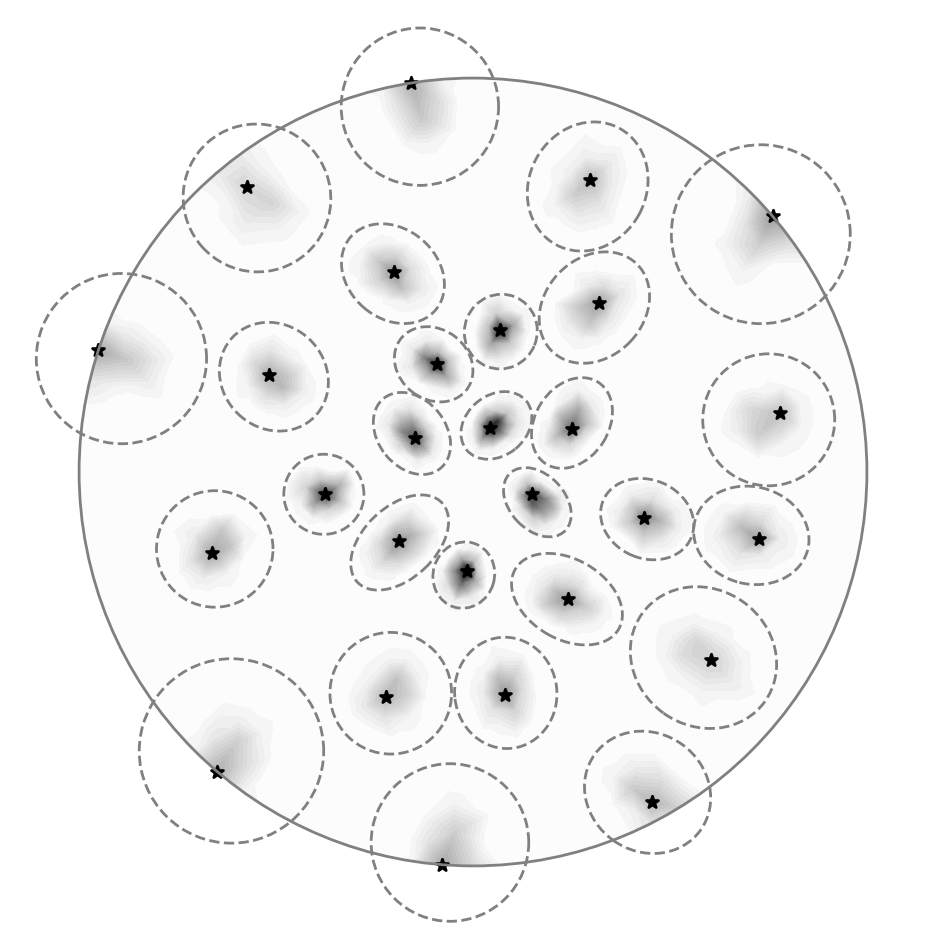
\includegraphics[scale=0.33]{impulse_batch1.png}
	\end{subfigure}
	\begin{subfigure}{0.32\textwidth}
		\centering
		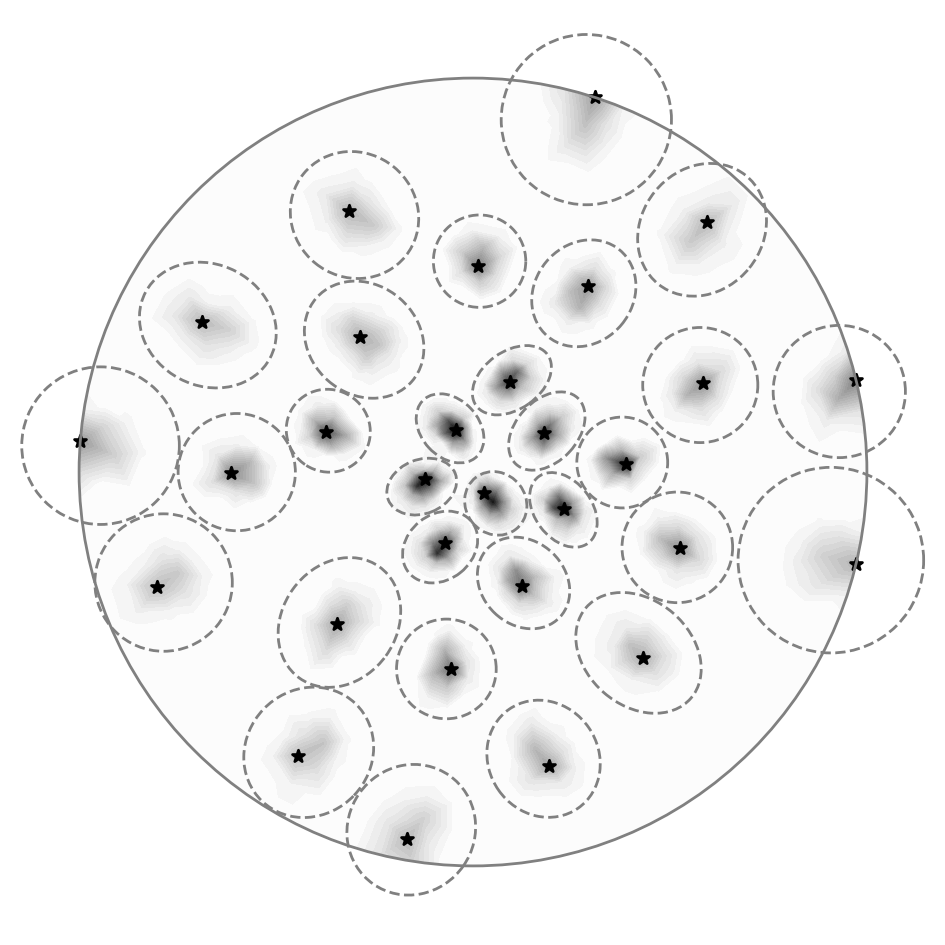
\includegraphics[scale=0.33]{impulse_batch2.png}
	\end{subfigure}
	\begin{subfigure}{0.32\textwidth}
		\centering
		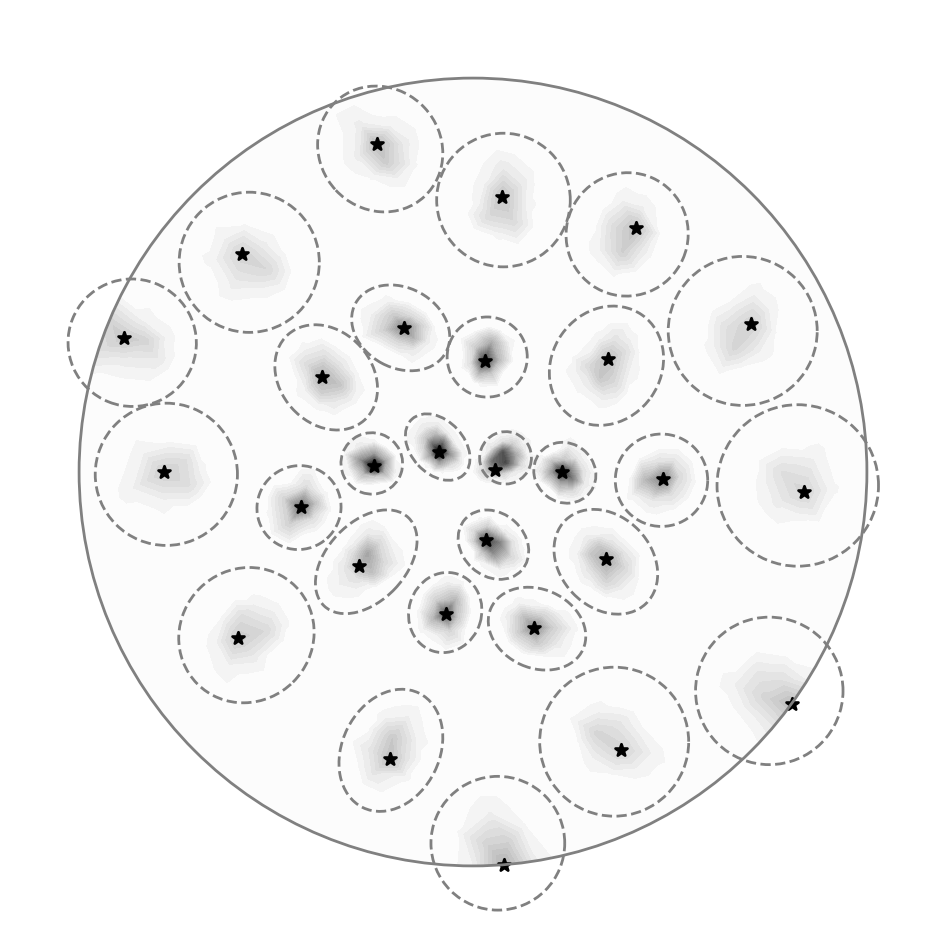
\includegraphics[scale=0.33]{impulse_batch3.png}
	\end{subfigure}
	\caption{Batches, $\eta_b$, of normalized impulses, $\impulseresponse_{x}$, for the Stokes inverse problem data misfit Gauss-Newton Hessian (Section~\ref{sec:numerical_results}). 
%	Brightness scale differs between the subfigures. 
	Black stars are point source locations. Dashed gray ellipses are estimated impulse response support ellipsoids. The large circle is $\partial \Omega$. 
	}
	\label{fig:batches_intro}
\end{figure}

%Existing scalable high rank approximation methods typically require the ability to rapidly evaluate arbitrary entries of $\Aop$'s integral kernel, which we cannot do. 
We use \emph{impulse response interpolation} to form a high rank operator approximation using a small number of operator applies. The impulse response, $\phi_x$, associated with a point $x$ is the Riesz representation\footnote{Recall that the Riesz representative of a functional $\rho \in L^2(\Omega)'$ with respect to the $L^2$ inner product is the unique function $\rho^* \in L^2(\Omega)$ such that $\rho(w) = \left(\rho^*,w\right)_{L^2(\Omega)}$ for all $w \in L^2(\Omega)$.} of the linear functional that results from applying $\Aop$ to a delta distribution (i.e., point source, impulse) centered at $x$. We compute batches of impulse responses by applying $\Aop$ to weighted sums of delta distributions associated with batches of points scattered throughout the domain (see Figure~\ref{fig:batches_intro}). Then we interpolate translated and scaled versions of these impulse responses to approximate entries of the operator's integral kernel. 
%This allows fast evaluation of approximate matrix entries, which are needed by high-rank approximation methods, in particular, classical H-matrix construction methods. 
Picking the batches of points requires us to estimate the supports of the impulse responses $\phi_x$ \emph{before} we compute them. 
The idea of estimating the supports of the functions $\phi_x$ a-priori was inspired by techniques from resolution analysis in seismic imaging. There, 
$\Aop^T$ is applied to a random noise function, and the width of $\phi_x$ is estimated to be the autocorrelation length of the resultant function near $x$~\cite{FichtnerLeeuwen15,TrampertFichtnerRitsema13}. We use polynomial functions instead of random noise functions (see Section~\ref{sec:intromoments}). Our method estimates the support of $\phi_x$ more accurately and reliably than random noise probing at the cost of the additional constraint that $\Aop$ has a non-negative integral kernel. Our method may be categorized as a PSF method that is loosely based on ``product convolution'' (PC) approximations, which are approximations of an operator by weighted sums of convolution operators with spatially varying weights. PC and PSF methods have a long history dating back several decades. We note the following papers (among many others), \cite{Adorf94,AlgerEtAl19,BigotEscandeWeiss19,EscandeWeiss15,EscandeWeiss22,EscandeWeiss12,FishEtAl96,NagyOleary98,ZhuLiFomelEtAl16}, in which the convolution kernels are constructed from sampling impulse responses of the operator to scattered point sources. For background on PC and PSF methods, we recommend the following papers: \cite{DenisEtAl15,EscandeWeiss17,GentileCourbinMeylan13}. While PC approximations are based on an assumption of local translation invariance, the method we propose is based on an assumption we call ``local mean displacement invariance,'' which is more general than local translation invariance, and includes both CUR low rank approximation and local translation invariance as special cases (Section~\ref{sec:local_mean_displacement_invariance} and Figure~\ref{fig:mean_displacement_invariance}). 
%Furthermore, PC approximations have well-known issues near boundaries due to so-called ``boundary artifacts,'' caused by the boundary artificially ``cutting off'' impulses. We avoid this issue by temporarily excluding impulses from the approximation procedure whenever an attempt is made to evaluate the impulse at a location where it is undefined. 

%\begin{figure}
%	\begin{center}
%		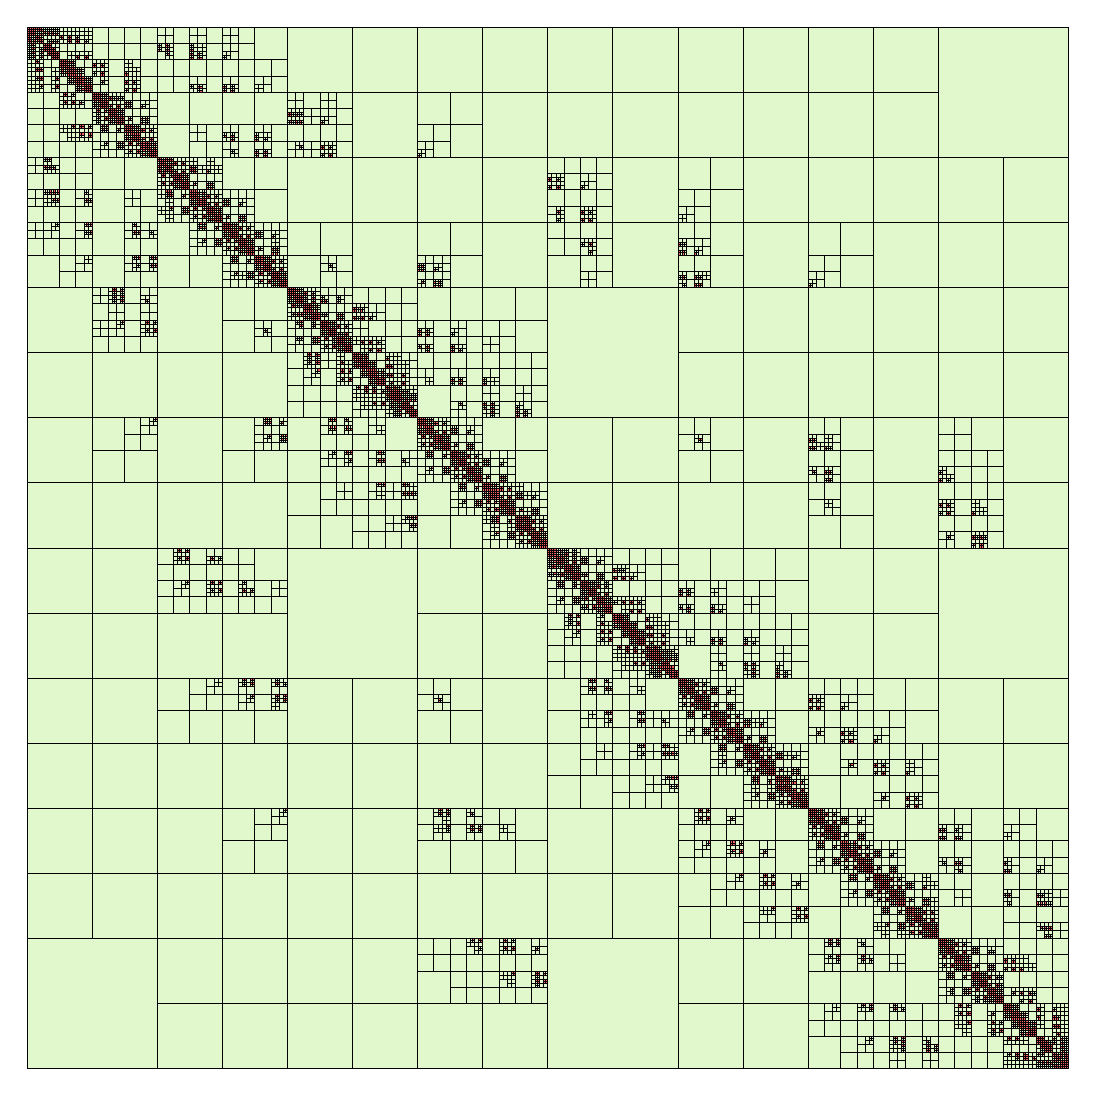
\includegraphics[scale=0.4]{bct1.eps}
%	\end{center}
%	\caption{Hierarchical matrix block structure for the Stokes Hessian. The red blocks (tiny) are dense. All other blocks are low rank.
%	}
%	\label{fig:hmatrix_intro}
%\end{figure}

\begin{figure}
	\begin{center}
		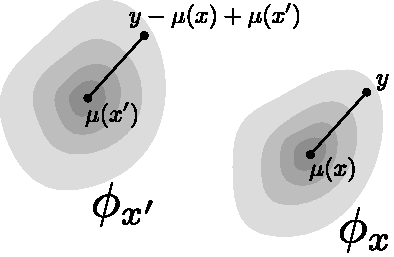
\includegraphics[scale=0.75]{mean_displacement_invariance.pdf}
	\end{center}
	\caption{$\Aop$ is locally mean displacement invariant if $\impulseresponse_{x}(y) \approx \impulseresponse_{x'}\left(y - \spatialmean(x) + \spatialmean(x')\right)$ when $x$ is close to $x'$. Here $\spatialmean(z)$ denotes the mean (center of mass) of $\phi_z$.}
	\label{fig:mean_displacement_invariance}
\end{figure}

The ability to rapidly approximate entries of $\Aop$'s integral kernel allows us to form a hierarchical matrix (H-matrix)~\cite{BormGrasedyckHackbusch03,Hackbusch99} approximation of a discretized version of $\Aop$. H-matrices are a matrix format in which the rows and columns of the matrix are re-ordered, then the matrix is recursively subdivided into blocks, in such a way that many off-diagonal blocks are low rank, even though the matrix as a whole may be high rank. 
%(see Figure~\ref{fig:hmatrix_intro} and Appendix~\ref{app:h_matrix}).
H-matrix methods permit us to perform matrix-vector products cheaply, and perform other useful linear algebra operations that cannot be done easily using the original operator. These operations include matrix-matrix addition, matrix-matrix multiplication, matrix factorization, and matrix inversion. 
%These H-matrix methods are fast and scale well to large problems. 
The work and memory required to perform these operations for an $\fedim \times \fedim$ H-matrix scales 
%as $O(\fedim \log(\fedim)^a)$, where $a \in \{0,1,2,3\}$. That is, the cost is \emph{nearly-linear}
\emph{nearly linearly} in $N$ (i.e., $o(N^{1+\epsilon})$ for any $\epsilon > 0$). The exact cost depends on the type of H-matrix used, the operation being performed, and the rank of the off-diagonal blocks~\cite{GrasedyckHackbusch03}. The ability to perform these operations permits, for example, fast solution of Newton linear systems in PDE constrained optimization, fast sampling of ill-conditioned posterior distribution in Bayesian inverse problems, and construction of high rank Gaussian surrogate models that can be used for uncertainty quantification. 
%Classical H-matrix construction methods 
%(described in Appendix~\ref{sec:H_matrix_construction}) 
%require access to matrix entries of the matrix being approximated, and therefore cannot be used to efficiently form H-matrix approximations of operators that are only available matrix free.


\section{Why we need high rank Hessian approximations}
\label{sec:hessian}

In distributed parameter inverse problems governed by PDEs, one seeks to infer an unknown spatially varying parameter field from limited observations of a state variable that depends on the parameter implicitly through the solution of a PDE. 
%Inverse problems are typically ill-posed, in the sense that many different parameter fields may yield predicted observations that agree with the actual observations to within the noise level. 
Conventionally, the inverse problem is formulated using either a deterministic framework~\cite{AsterBorchersThurber18,Vogel02},
%Guy Chavent, Nonlinear Least Squares for Inverse Problems, Springer, 2009.
or a Bayesian probabilistic framework~\cite{KaipioSomersalo05,Stuart10a,Tarantola05}. In the deterministic framework, one solves an optimization problem to find the parameter that best fits the observations, subject to appropriate regularization~\cite{EnglHankeNeubauer96}. In the probabilistic framework, Bayes' theorem combines the observations with prior information to form a posterior distribution over the space of all possible parameter fields, and computations are performed to extract statistical information about the parameter from this posterior. The Hessian of the objective function in the determinstic optimization problem and the Hessian of the negative log posterior in the Bayesian setting are equal or approximately equal to each other under typical noise, regularization, and prior models, so we refer to both of these Hessians as ``the Hessian.'' The Hessian consists of a data misfit term (the ``data misfit Hessian''), which depends on discrepancy between the observations and the associated model predictions, and a regularization or prior term (the ``regularization Hessian'') which does not depend on the observations. For more details on the Hessian, see~\cite{Alger19,GhattasWillcox21,VillaPetraGhattas21}. 

Hessian approximations and preconditioners are highly desirable because the Hessian is central to efficient solution of inverse problems in both the deterministic and Bayesian settings. When solving the deterministic optimization problem with Newton-type methods, the Hessian is the coefficient operator for the linear system that must be solved or approximately solved at every Newton iteration. Good Hessian preconditioners reduce the number of iterations required to solve these Newton linear systems with Krylov methods such as conjugate gradient~\cite{Saad03}. In the Bayesian setting, the inverse of the Hessian is the covariance of a local Gaussian approximation of the posterior. Such a Gaussian distribution can be used as a direct approximations of the posterior, or as a proposal for Markov chain Monte-Carlo methods for drawing samples from the posterior. For instance, see~\cite{KimEtAl21,PetraEtAl14} and the references therein. 

%\begin{figure}
%	\begin{subfigure}{0.5\textwidth}
%		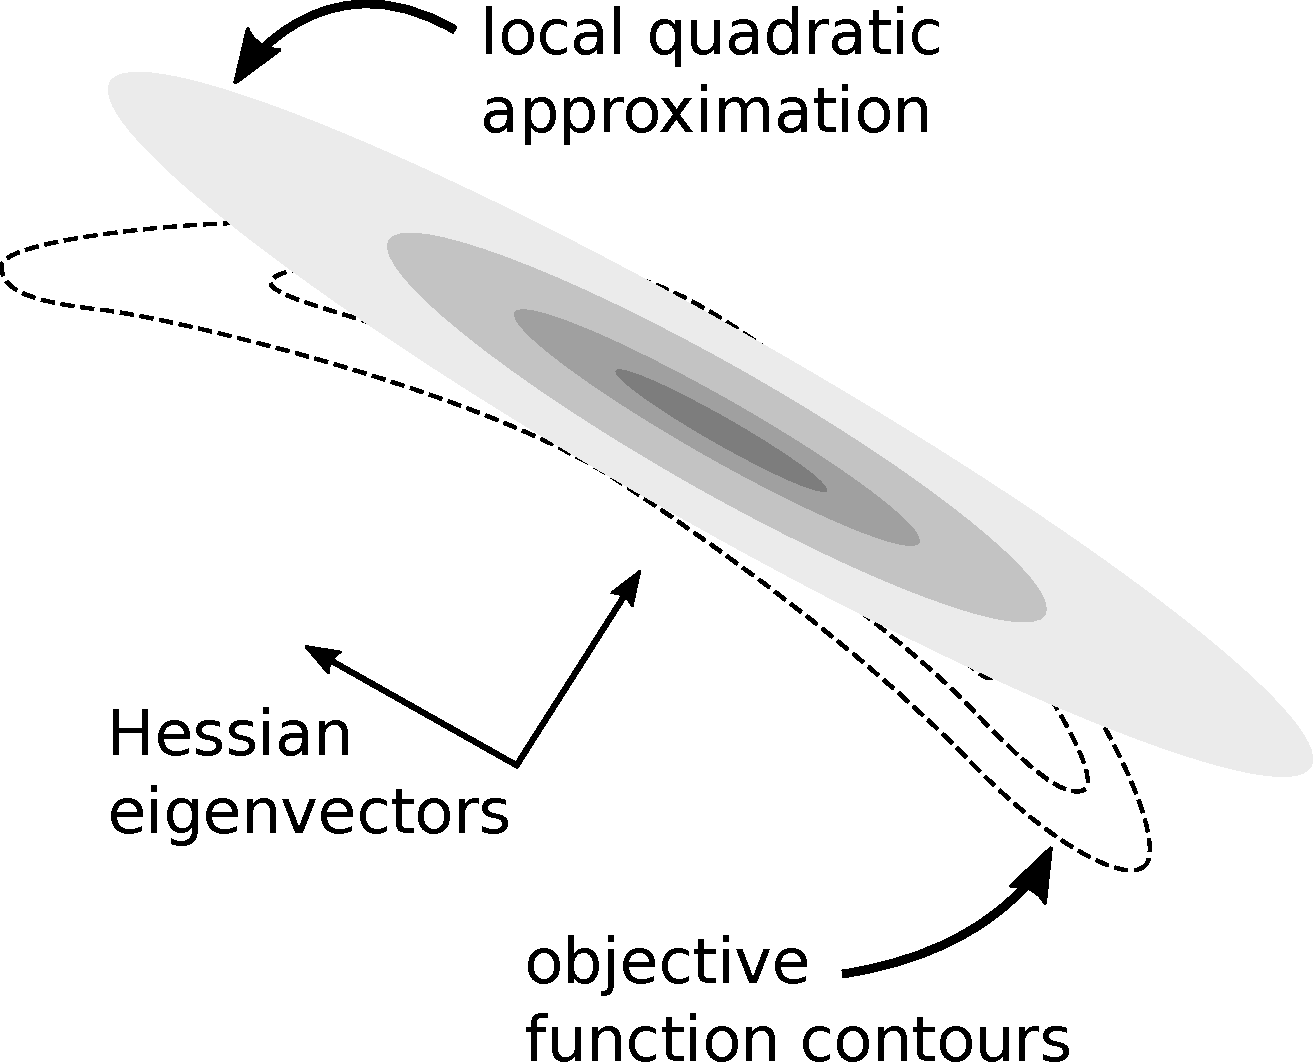
\includegraphics[scale=0.23]{informed_uninformed_modes_quadratic.pdf}
%		\caption{}
%	\end{subfigure}
%	\begin{subfigure}{0.48\textwidth}
%		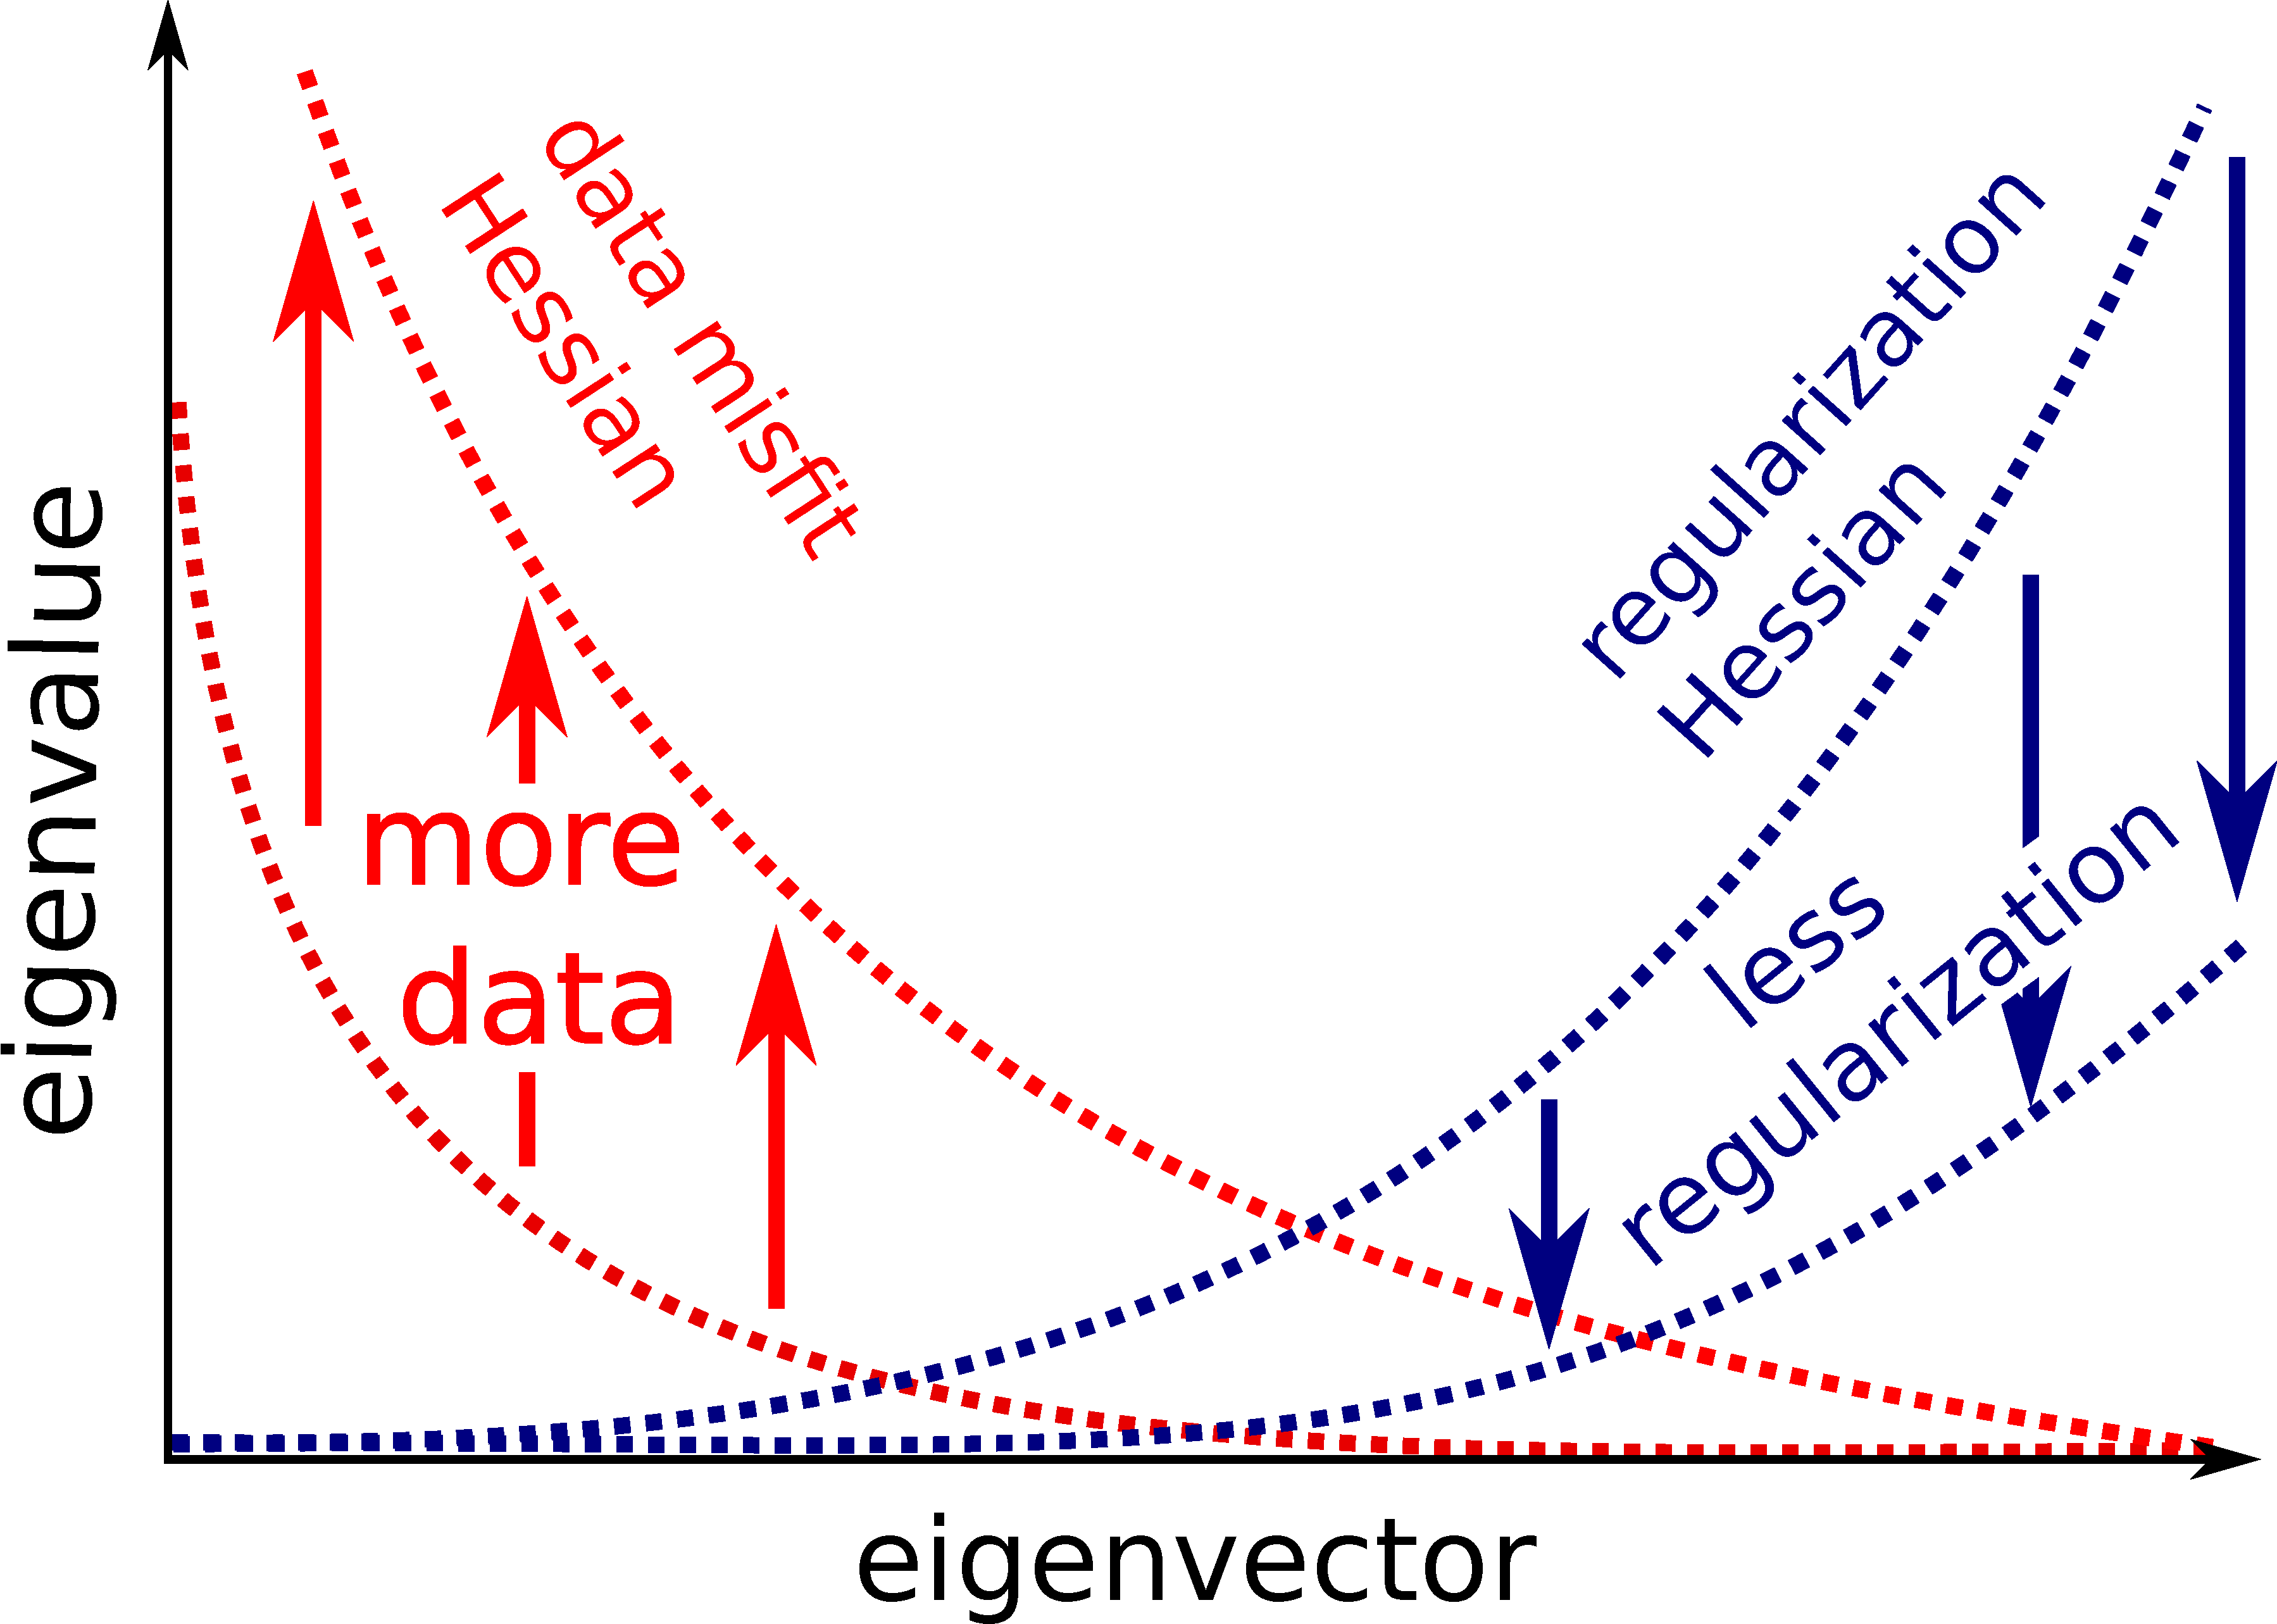
\includegraphics[scale=0.1]{misfit_and_reg_hessian_eigenvalues.pdf}
%		\caption{}
%	\end{subfigure}
%	\caption{(a) The Hessian eigenstructure characterizes the directional scalings of the best local quadratic approximation to the objective function in an inverse problem. The larger an eigenvalue of the Hessian is, the more closely spaced the contours of the local quadratic approximation are in the corresponding eigenvector direction. (b) As the data in an inverse problem becomes more informative about the parameter, the eigenvalues of the data misfit Hessian increase. As the regularization is weakened, the eigenvalues of the regularization Hessian decrease. These illustrations are taken from~\cite[Chapter 1]{Alger19}, with minor modifications.}
%	\label{fig:hessian_eigenstructure}
%\end{figure} 


Owing to the implicit dependence of predicted observations on the parameter, entries of the Hessian are not easily accessible. Rather, the Hessian may be applied to a vector via a computational process that involves solving a pair of forward and adjoint PDEs which are linearizations of the original PDE~\cite{GhattasWillcox21,Gunzburger03}. The most popular matrix-free Hessian approximation methods are based on low rank approximation of either the data misfit Hessian, or the data misfit Hessian preconditioned by the regularization Hessian, e.g.,~\cite{BuiEtAl13,CuiEtAl14,FlathEtAl11,PetraEtAl14,SpantiniEtAl15}. Krylov methods such as Lanczos or randomized methods~\cite{Cheng05,HalkoMartinssonTropp11} are typically used to construct these low rank approximations by applying the Hessian to vectors. Using these methods, the required number of Hessian applications (and hence the required number of PDE solves) is typically proportional to the rank of the low rank approximation. Low rank approximation methods are justified by arguing that the numerical rank of the data misfit Hessian is insensitive to the dimension of the discretized parameter. This means that the required number of PDE solves remains the same as the mesh used to discretize the parameter is refined.
However, in many inverse problems of practical interest the numerical rank of the data misfit Hessian, while mesh independent, is still large, which makes it costly to approximate the Hessian using low rank approximation methods~\cite{AmbartsumyanEtAl20,BuiEtAl13,IsaacEtAl15}. 

Examples of inverse problems with high rank data misfit Hessians include advection dominated advection-diffusion inverse problems~\cite{AkcelikBirosDraganescuEtAl05}\cite[Chapter 5]{Flath13}, high frequency wave inverse problems~\cite{BuiEtAl13}, and more generally, all inverse problems in which the observations highly inform the parameter. The eigenvalues of the data misfit Hessian characterize the sensitivity of the predicted observations to perturbations of the parameter in the corresponding eigenvector directions,
%(see Figure~\ref{fig:hessian_eigenstructure})
so more informative data leads to larger eigenvalues and therefore a larger numerical rank~\cite{AlexanderianGloorGhattas16}\cite[Section 1.4 and Chapter 4]{Alger19}. Roughly speaking, the numerical rank of the data misfit Hessian is the dimension of the subspace of parameter space that is informed by the data. The numerical rank of the regularization preconditioned data misfit Hessian may be reduced by increasing the strength of the regularization, but this throws away useful information---components of the parameter that could be learned from components of the observations that have a large signal to noise ratio are instead reconstructed based on the regularization~\cite[Section 4]{AlgerEtAl17}\cite[Chapters 1 and 7]{Vogel02}. Hence, low rank approximation methods suffer from a predicament---if the data highly inform the parameter and the regularization is chosen appropriately, then a large number of operator applies are required to form an accurate approximation of the Hessian using low rank approximation methods. 
%The best case scenario from a scientific perspective (highly informative data) is the worst case scenario from a computational perspective (large computational cost)~\cite{AlexanderianGloorGhattas16,Alger19,AlgerEtAl17}. 
High rank Hessian approximation methods are needed.

Recently there have been improvements in matrix-free H-matrix construction methods in which an operator is applied to structured random vectors, and the response of the operator to those random vectors is processed to construct an H-matrix approximation~\cite{LevittMartinsson22,LinYing11,Martinsson11,Martinsson16,MartinssonTropp20}. 
These methods (which we do not use here) have been used to approximate Hessians in PDE constrained inverse problems~\cite{AmbartsumyanEtAl20,HartlandEtAl23}. 
Although the required number of matrix-vector products grows nearly linearly in the discretized parameter dimension and linearly in the rank of the off-diagonal blocks, the required number of matrix-vector products is still large (e.g., hundreds to thousands).
%These methods are asymptotically scalable in the sense that the required number of matrix-vector products grows nearly linearly in the dimension of the discretized parameter and linearly in the rank of the off-diagonal blocks. But despite asymptotic scalability, from a practical perspective the required number of matrix-vector products is large (e.g., hundreds to thousands). 
%Improving the peeling process to reduce its cost is currently an area of active research~\cite{PEELINGRESEARCH}.
%This is an area of active research, so more efficient and practical matrix-free H-matrix construction methods based on the peeling process may be discovered in the future.
%Matrix-free H-matrix construction methods are currently an area of active research (see, e.g.,~\cite{LevittMartinsson22}), so more efficient matrix-free H-matrix methods may be discovered in the future. 
In this paper, we also form an H-matrix Hessian approximation. However, to reduce the required number of operator actions, we first form a PSF approximation of the data misfit Hessian by exploiting locality and non-negative integral kernel properties, then form the H-matrix using classical H-matrix techniques. Not all data misfit Hessians satisfy the local non-negative integral kernel properties (for example, the wave inverse problem data misfit Hessian has a substantial amount of negative entries in its integral kernel). However, many data misfit Hessians of practical interest do satisfy these properties (either exactly or approximately), and our method is targeted at approximating these Hessians.

%Classical methods for approximating the Hessian are based on low rank approximation of either the data misfit Hessian, or the data misfit Hessian preconditioned by the inverse of the prior term in the Hessian. However,  More generally, the eigenvalues of the Hessian characterize how informative the data are about the component of the parameter in the corresponding parameter direction. The more informed the component of the parameter, the larger

%In the deterministic setting, the Hessian of the objective function is central to efficient solution of the optimization problem, and in the 

% given the observed data is  one explores the posterior probability distribution for the parameter

%Our motivation is high rank Hessian approximation in distributed parameter inverse problems governed by PDEs. 
%The Hessian is an operator that is central to efficient methods for solving such inverse problems and is only available matrix-free; we will discuss Hessians in inverse problems governed by PDEs in greater detail in Section~\ref{sec:hessian}.

%Introduce inverse problem
%
%Role of Hessian
%
%Structure of Hessian that we want to exploit
%
%Low rank
%
%Need for High rank
%
%Low rank approximation of the Hessian:
%\begin{itemize} 
%	\item Hessian eigenstructure is determined by data informativeness. Bigger eigenvalue => more informed component in eigenvector direction. 
%	\item informative data => high rank hessian
%	\item get high rank approximation by exploiting different structure. Locality, non-negativity of kernel
%	\item Large rank in absolute terms, even if low rank in relative terms
%\end{itemize}




\section{Preliminaries}

Let $\Omega \subset \mathbb{R}^\gdim$ be a bounded domain (typically $\gdim=1$, $2$, or $3$). We seek to approximate integral operators $\Aop:L^2(\Omega)\rightarrow L^2(\Omega)'$ of the form
\begin{equation}
\label{eq:kernel_representation}
(\Aop u)(w) := \int_\Omega \int_\Omega w(y) \Aker(y,x) u(x) dx dy.
\end{equation}
Here the linear functional $\Aop u \in L^2(\Omega)'$ is the result of applying $\Aop$ to $u\in L^2(\Omega)$, the scalar $\left(\Aop u\right)(w)$ is the result of applying that linear functional to $w \in L^2(\Omega)$.
The integral kernel, $\Aker:\Omega \times \Omega \rightarrow \mathbb{R}$, exists in principle but is not easily accessible. In this section we describe how to extend the action of $\Aop$ to distributions, which allows us to define impulse responses (Section~\ref{sec:impulse_response_2}), we state the conditions on $\Aop$ that our method requires (Section~\ref{sec:conditions_2}), and we detail finite element discretization (Section~\ref{sec:finite_element_kernel}).

\subsection{Distributions and impulse responses}
\label{sec:impulse_response_2}

The action of $\Aop$ may be extended to distributions if $\Aker$ is sufficiently regular. 
%We derive the extension as follows. 
Let $\rho \in L^2(\Omega)'$, and let $\rho^* \in L^2(\Omega)$ denote the Riesz representative of $\rho$ with respect to the $L^2(\Omega)$ inner product. We have
\begin{subequations}
	\label{eq:extension_to_distributions}
	\begin{align}
		\left(\Aop \genericdistribution^*\right)(w) &= \int_\Omega \int_\Omega w(y) \Aker(y,x) \genericdistribution^*(x) dx ~dy \\
		&= \int_\Omega w(y) \int_\Omega \Aker(y,x) \genericdistribution^*(x) dx ~dy 
		= \int_\Omega w(y) \genericdistribution\left(\Aker(y,\cdot)\right) dy, \label{eq:action_on_distribution}
	\end{align}
\end{subequations}
where $\Aker(y,\cdot)$ denotes the function $x \mapsto \Aker(y,x)$.
Now let $\mathcal{D}(\Omega) \subset L^2(\Omega)$ be a suitable space of test functions and let $\rho:\mathcal{D}(\Omega) \rightarrow \mathbb{R}$ be a distribution. In this case, the Riesz representative $\rho^*$ may not exist, so the derivation in~\eqref{eq:extension_to_distributions} is not valid. However, if $\Aker$ is sufficiently regular such that the function $y \mapsto \rho\left(\Aker(y,~\cdot~)\right)$ is well defined for almost all $y\in\Omega$, and if this function is in $L^2(\Omega)$, then the right hand side of~\eqref{eq:action_on_distribution} is well defined. Hence, we \emph{define} the action of $\Aop$ on the distribution $\rho$ to be the right hand side of~\eqref{eq:action_on_distribution}. We denote this action by ``$\Aop \genericdistribution^*$,'' even if $\rho^*$ does not exist.

Let $\delta_x$ denote the delta distribution\footnote{Recall that the delta distribution $\delta_x:\mathcal{D}(\Omega)\rightarrow \mathbb{R}$ is defined by $\delta_x(w) = w(x)$ for all $w\in \mathcal{D}(\Omega)$.} (i.e., point source, impulse) centered at the point $x \in \Omega$.
The \emph{impulse response} of $\Aop$ associated with $x$ is the function $\impulseresponse_x:\Omega \rightarrow \mathbb{R}$, 
\begin{equation}
\label{eq:impulse_response_delta_action}
\impulseresponse_x := \left( \Aop \delta_x^* \right)^*,
\end{equation}
that is formed by applying $\Aop$ to $\delta_x$, then taking the Riesz representation of the resulting linear functional. Using~\eqref{eq:action_on_distribution} and the definition of the delta distribution, we see that $\phi_x$ may also be written as the function $\impulseresponse_x(y) = \Aker(y, x)$.
%\begin{equation}
%\label{eq:impulse_response_defn}
%\impulseresponse_x(y) = \Aker(y, x),
%\end{equation} 
%which results from keeping $x$ fixed and viewing $\Aker(y,x)$ as a function of $y$. 

\subsection{Required conditions}
\label{sec:conditions_2}

We focus on approximating operators that satisfy the following conditions: 
\begin{enumerate}
	\item The kernel $\Aker$ is sufficiently regular so that $\phi_x$ is well defined for all $x\in \Omega$.
	\item The supports of the impulse responses $\impulseresponse_x$ are contained in localized regions.
	\item The integral kernel is non-negative in the sense that $$\Aker(y,x) \ge 0$$ for all $(y,x) \in \Omega \times \Omega$.\footnote{Note that having a non-negative integral kernel is different from positive semi-definiteness. The operator $\Aop$ need not be positive semi-definite to use our method, and positive semi-definite operators need not have a non-negative integral kernel.}
\end{enumerate}
Our method may still perform well if these conditions are relaxed slightly. It is fine if the support of $\impulseresponse_x$ is not perfectly contained in a localized region, as long as the bulk of the ``mass'' of $\impulseresponse_x$ is contained in a localized region. The integral kernel does not need to be non-negative for all pairs of points $(y,x) \in \Omega \times \Omega$, as long as it is non-negative for the vast majority of pairs of points $(y,x)$, and as long as the negative numbers are comparatively small. If these conditions are violated, our method will incur additional error. If these conditions are violated too much, our method may fail. 
%Not all operators of interest (and in particular not all Hessians) satisfy these conditions, but many operators of practical interest do satisfy these conditions, and our method is highly effective for approximating these operators.

\subsection{Finite element discretization}
\label{sec:finite_element_kernel}

In computations, functions are discretized and replaced by finite dimensional vectors, and operators mapping between infinite dimensional spaces are replaced by operators mapping between finite dimensional spaces. In this paper we discretize using continuous Galerkin finite elements satisfying the Kronecker property (defined below). With minor modifications, our method could be used with more general finite element methods, or other discretization schemes such as finite differences or finite volumes.

Let $\febasis_1, \febasis_2, \dots, \febasis_\fedim$ be a set of continuous Galerkin finite element basis functions used to discretize the problem on a mesh with mesh size parameter $h$, let $V_h := \Span\left(\febasis_1, \febasis_2, \dots, \febasis_\fedim\right)$ be the corresponding finite element space under the $L^2$ inner product, and let $\fepoint_i \in \mathbb{R}^\gdim$, $i=1,\dots, \fedim$ be the Lagrange nodes associated with the functions $\febasis_i$. We assume that the finite element basis satisfies the Kronecker property, i.e., $\febasis_i(\fepoint_i)=1$ and $\febasis_i(\fepoint_j)=0$ if $i\neq j$. 
For $u_h \in V_h$ we write $\bm{u} \in \mathbb{R}^\nsamplepts_\massmatrix$ to denote the coefficient vector for $u_h$ with respect to the finite element basis, i.e.,
$
%\label{eq:fem_coeff_basis}
u_h(x) = \sum_{i=1}^\fedim \bm{u}_i \febasis_i(x).
$
Linear functionals $\rho_h \in V_h'$ have coefficient dual vectors $\boldsymbol{\rho}\in \mathbb{R}^\nsamplepts_{\massmatrix^{-1}}$, with entries $\boldsymbol{\rho}_i = \rho_h(\febasis_i)$ for $i=1,\dots,\nsamplepts$.
%\begin{equation*}
%\boldsymbol{\rho}_i = \rho_h(\febasis_i), \qquad i=1,\dots,\nsamplepts. 
%\end{equation*}
Here $\massmatrix \in \mathbb{R}^{\fedim \times \fedim}$ denotes the sparse finite element mass matrix which has entries $\massmatrix_{ij}=\int_\Omega \febasis_i(x) \febasis_j(x) dx$ for $i,j=1,\dots,\fedim$.
%\begin{equation*}
%\massmatrix_{ij}=\int_\Omega \febasis_i(x) \febasis_j(x) dx, \qquad i,j=1,\dots,\fedim,
%\end{equation*}
The space $\mathbb{R}^\fedim_\massmatrix$ is $\mathbb{R}^\fedim$ with the inner product $(\mathbf{u},\mathbf{w})_\massmatrix := \mathbf{u}^T \massmatrix \mathbf{w}$, and $\mathbb{R}^\fedim_{\massmatrix^{-1}}$ is the analogous space with $\massmatrix^{-1}$ replacing $\massmatrix$. Direct calculation shows that $\mathbb{R}^\fedim_\massmatrix$ and $\mathbb{R}^\fedim_{\massmatrix^{-1}}$ are isomorphic to $V_h$ and $V_h'$ as Hilbert spaces, respectively.

After discretization, the operator $\Aop:L^2(\Omega) \rightarrow L^2(\Omega)'$ is replaced by an operator $A_h:V_h \rightarrow V_h'$, which becomes an operator
\begin{equation*}
\mathbf{A}:\mathbb{R}^\fedim_\massmatrix \rightarrow \mathbb{R}^\fedim_{\massmatrix^{-1}}
\end{equation*}
under the isomorphism discussed above. Our method is agnostic to the computational procedure for approximating $\Aop$ with $\mathbf{A}$. What is important is that we do not have direct access to matrix entries $\mathbf{A}_{ij}$. Rather, we have a computational procedure that allows us to compute matrix-vector products $\mathbf{u}\mapsto \mathbf{A}\mathbf{u}$ and $\mathbf{w}\mapsto \mathbf{A}^T\mathbf{w}$, and computing these matrix-vector products is costly.
Of course, matrix entries can be computed via matrix-vector products as $\mathbf{A}_{ij} = \left(\mathbf{A}\mathbf{e}_j\right)_i$,
where $\mathbf{e}_j=(0,\dots,0,1,0,\dots,0)^T$ is the length $\fedim$ unit vector with one in the $j$th coordinate and zeros elsewhere. But computing the matrix-vector product $\mathbf{e}_j \mapsto \mathbf{A}\mathbf{e}_j$ is costly, and therefore wasteful if we do not use other matrix entries in the $j$th column of $\mathbf{A}$. Hence, methods for approximating $\mathbf{A}$ are computationally intractable if they require accessing scattered matrix entries from many different rows and columns of $\mathbf{A}$. 

The operator $A_h:V_h \rightarrow V_h'$ can be written in integral kernel form,~\eqref{eq:kernel_representation}, but with $\Aker$ replaced by a slightly different integral kernel,
%as
%\begin{equation}
%(A_h u_h)(w_h) := \int_\Omega \int_\Omega w_h(y) \Aker_h(y,x) u_h(x) dx dy
%\end{equation}
$\Aker_h$, which we do not know, and which differs from $\Aker$ due to discretization error. Since the functions in $V_h$ are continuous at $x$, the delta distribution $\delta_x$ is a continuous linear functional on $V_h$, which has a discrete dual vector $\boldsymbol{\delta}_x \in \mathbb{R}^\fedim_{\massmatrix^{-1}}$ with entries $\left(\boldsymbol{\delta}_x\right)_i = \febasis_i(x)$ for $i=1,\dots,\fedim$. Additionally, it is straightforward to verify that the Riesz representation, $\rho_h^* \in V_h$, of a functional $\rho \in V_h'$ has coefficient vector
$
\boldsymbol{\rho}^* = \massmatrix^{-1} \boldsymbol{\rho}.
$
Therefore, the formula for the impulse response from~\eqref{eq:impulse_response_delta_action} becomes 
$
%\label{eq:discrete_kernel}
\boldsymbol{\impulseresponse}_x = \left(A_h \delta_x^*\right)^* =  \massmatrix^{-1}\mathbf{A} \massmatrix^{-1} \boldsymbol{\delta}_x,
$
and the $(y,x)$ kernel entry of $\Aker_h$ may be written as
$
%\label{eq:approx_kernel_entry_81}
	\Aker_h(y,x) = \boldsymbol{\delta}_y^T \boldsymbol{\impulseresponse}_x = \boldsymbol{\delta}_y^T \massmatrix^{-1}\mathbf{A} \massmatrix^{-1} \boldsymbol{\delta}_x.
$
Now define $\mathbf{\Aker} \in \mathbb{R}^{\fedim \times \fedim}$ to be the following dense matrix of kernel entries evaluated at all pairs of Lagrange nodes:
\begin{equation}
\label{eq:Akerpcmat_entries}
\mathbf{\Aker}_{ij} := \Aker_h(\fepoint_i, \fepoint_j).
\end{equation}
Because of the Kronecker property of the finite element basis, we have $\boldsymbol{\delta}_{\fepoint_i} = \mathbf{e}_i$. Thus, we have
$
	\Aker_h(\fepoint_i,\fepoint_j) = \left(\massmatrix^{-1}\mathbf{A} \massmatrix^{-1}\right)_{ij},
$
which implies
\begin{equation}
\label{eq:boldA}
	\mathbf{A} = \massmatrix \mathbf{\Aker} \massmatrix.
\end{equation}
Broadly, our method will construct an H-matrix approximation of $\mathbf{A}$ by forming H-matrix approximations of $\boldsymbol{\Aker}$ and $\massmatrix$ (or a lumped mass version of $\massmatrix$), then multiplying these matrices per~\eqref{eq:boldA} using H-matrix methods. Classical H-matrix construction methods require access to arbitrary matrix entries $\mathbf{\Aker}_{ij}$, but these matrix entries are not easily accessible. The bulk of our method is therefore dedicated to forming approximations of these matrix entries that can be evaluated rapidly.

\paragraph{Lumped mass matrix} At the continuum level, $\Aker$ is assumed to be non-negative. However, entries of $\Aker_h$, involve inverse mass matrices, which typically contain negative numbers. If there are too many negative numbers, or if the negative numbers are too large, our algorithm will be less robust. We therefore recommend replacing the mass matrix, $\massmatrix$, with a positive diagonal \emph{lumped mass} approximation. 
In our numerical results, we use the lumped mass matrix constructed by replacing off-diagonal entries of the mass matrix by zero. Other mass lumping techniques may be used~\cite{Hughes12}.


\section{Key innovations}
\label{sec:prerequisites}

In this section we present two key innovations that our method is based on.
First, we define moments of the impulse responses, $\phi_x$, show how these moments can be computed efficiently, and use these moments to form ellipsoid shaped a-priori estimates for the supports of the impulse responses (Section~\ref{sec:intromoments}). 
%Our method will use these ellipsoid estimates to choose sets of impulses that can be computed in batches. 
Second, we describe an improved method of approximating impulse responses by other nearby impulse responses, which we call ``normalized local mean displacement invariance'' (Section~\ref{sec:local_mean_displacement_invariance}). 
%Our method will interpolate impulses using this approximation. 



\subsection{Impulse response moments and ellipsoid support estimate}
\label{sec:intromoments}

The impulse response $\impulseresponse_x$ may be interpreted as a scaled probability distribution because of the non-negative integral kernel property. Let $\spatialvol:\Omega \rightarrow \mathbb{R}$,
\begin{equation}
\label{eq:define_vol}
\spatialvol(x) := \int_\Omega \impulseresponse_x(y) dy
\end{equation}
denote the spatially varying scaling factor, and for $i,j=1,\dots,\gdim$ define $\spatialmean:\Omega \rightarrow \mathbb{R}^\gdim$ and $\spatialcov:\Omega \rightarrow \mathbb{R}^{\gdim \times \gdim}$ as follows:
\begin{align}
\spatialmean^i(x) :=& \int_\Omega (\impulseresponse_x(y) / V(x)) y^i ~dy \label{eq:define_mean} \\
\spatialcov^{ij}(x) :=& \int_\Omega (\impulseresponse_x(y) / V(x)) \left(y^i - \spatialmean^i(x)\right) \left(y^j - \spatialmean^j(x)\right) ~dy, \label{eq:define_cov}
\end{align}
where $\spatialmean^i(x)$ denotes the $i^\text{th}$ component of the vector $\spatialmean(x)$, and $\spatialcov^{ij}(x)$ denotes the $(i,j)$ entry of the matrix $\spatialcov(x)$.
The vector $\spatialmean(x)\in \mathbb{R}^\gdim$ and the matrix $\spatialcov(x) \in \mathbb{R}^{\gdim \times \gdim}$ are the mean and covariance of the normalized version of $\impulseresponse_x$, respectively. 

The direct approach to compute $\spatialvol(x)$, $\spatialmean(x)$, and $\spatialcov(x)$ is to apply $\Aop$ to a point source centered at $x$ to obtain $\impulseresponse_x$, as per~\eqref{eq:impulse_response_delta_action}. Then one can post process $\impulseresponse_x$ to determine $\spatialvol(x)$, $\spatialmean(x)$, and $\spatialcov(x)$. However, this direct approach is not feasible because we need to know $V(x)$, $\spatialmean(x)$, and $\spatialcov(x)$ before we compute $\phi_x$, in order choose the point $x$. Computing $\phi_x$ in order to determine $V(x)$, $\spatialmean(x)$, and $\spatialcov(x)$ would be extremely computationally expensive, and defeat the purpose of our algorithm, which is to reduce the computational cost by computing impulse responses in batches. Fortunately, it is possible to compute $\spatialvol(x)$, $\spatialmean(x)$, and $\spatialcov(x)$ indirectly, \emph{for all points $x\in\Omega$ simultaneously}, by applying $\Aop^T$ to one constant function, $\gdim$ linear functions, and $\gdim(\gdim+1)/2$ quadratic functions (e.g., 6 total operator applies in two spatial dimensions and 10 in three spatial dimensions). This may be motivated by analogy to matrices. If $\mathbf{B}\in \mathbb{R}^{\fedim \times \fedim}$ is a matrix with $i^\text{th}$ column $\mathbf{b}_i$ and $\mathbf{w} \in \mathbb{R}^\fedim$, then
\begin{equation*}
\mathbf{B}^T \mathbf{w} = \begin{bmatrix}
\horzbar & \mathbf{b}_1^T & \horzbar \\
%\horzbar & \mathbf{b}_2^T & \horzbar \\
& \vdots & \\
\horzbar & \mathbf{b}_\fedim^T & \horzbar
\end{bmatrix}
\mathbf{w} = 
\begin{bmatrix}
\mathbf{b}_1^T \mathbf{w} \\
%\mathbf{b}_2^T \mathbf{w} \\
\vdots \\
\mathbf{b}_\fedim^T \mathbf{w}
\end{bmatrix}.
\end{equation*}
By computing one matrix-vector product of $\mathbf{B}^T$ with $\mathbf{w}$, we compute the inner product of each column of $\mathbf{B}$ with $\mathbf{w}$ simultaneously. The operator case is analogous, with $\phi_x$ taking the place of a matrix column. We have
\begin{equation}
\label{eq:operator_simultaneous_ips}
\left(\Aop^T w\right)^*(x) = \int_\Omega \Aker(y,x) w(y) dy = \left(\phi_x, w\right)_{L^2(\Omega)}.
\end{equation}
By computing one operator application of $\Aop^T$ to $w$, we compute the inner product of each $\phi_x$ with $w$, for all points $x$ simultaneously. 

Let $C$, $L^i$, and $Q^{ij}$ be the following constant, linear, and quadratic functions:
\begin{equation*}
C(x) := 1, \qquad
L^i(x) := x^i, \qquad
Q^{ij}(x) := x^i x^j
\end{equation*}
for $i,j=1,\dots,\gdim$. Using the definition of $\spatialvol$ in~\eqref{eq:define_vol} and using~\eqref{eq:operator_simultaneous_ips}, we have
\begin{equation*}
	\spatialvol(x) = \int_\Omega \phi_x(y) C(y) ~ dy = \left(\phi_x, C\right)_{L^2(\Omega)} = \left(\mathcal{A}^T C\right)^*(x).
\end{equation*}
Hence, we compute $\spatialvol(x)$ for all $x$ simultaneously by applying $\Aop^T$ to $C$. Analogous manipulations show that $\spatialmean(x)$ and $\spatialcov(x)$ may be computed for all points $x$ simultaneously by applying $\Aop^T$ to the functions $L^i$ and $Q^{ij}$, respectively. We have
\begin{subequations}
	\label{eq:vol_mean_var}
	\begin{align}
	\spatialvol =& \left(\Aop^T C\right)^* \\
	\spatialmean^i =& \left(\Aop^T L^i\right)^* / \spatialvol \\
	\spatialcov^{ij} =& \left(\Aop^T Q^{ij}\right)^* / \spatialvol - \spatialmean^i\cdot \spatialmean^j
	\end{align}
\end{subequations}
for $i,j=1,\dots, \gdim$. Here $u/w$ denotes pointwise division, $\left(u/w\right)(x) = u(x)/w(x)$, and $u\cdot w$ denotes pointwise multiplication, $(u \cdot w)(x) = u(x)w(x)$.
%The resulting method for computing discretized versions of $\spatialvol$, $\spatialmean$, and $\spatialcov$ is shown in Algorithm~\ref{alg:varhpi_mean_cov}.

%\begin{algorithm2e}
%	\SetAlgoNoLine
%	\SetKwInOut{Input}{Input}
%	\SetKwInOut{Output}{Output}
%	{	
%		\Input{Operator $\bm{A}^T$}
%		\Output{$\bm{\spatialvol}\in \mathbb{R}^\fedim$, $\bm{\spatialmean}\in \mathbb{R}^{\gdim \times \fedim}$, and $\bm{\spatialcov} \in \mathbb{R}^{\gdim \times \gdim \times \fedim}$}
%		
%		Form vector $\bm{C} \in \mathbb{R}^\fedim_{\massmatrix}$ by either projecting or interpolating constant function $C(x)=1$ onto $V_h$
%		
%		$\bm{\spatialvol} \gets \massmatrix^{-1}\bm{A}^T \bm{C}$
%		
%		\For{$i=1,2,\dots,\gdim$}{
%			Form vector $\bm{L}^i \in \mathbb{R}^\fedim_{\massmatrix}$ by either projecting or interpolating linear function $L^i(x) = x^i$ onto $V_h$
%			
%			$\bm{\spatialmean}^i \gets \left(\massmatrix^{-1}\bm{A}^T \bm{L}^i\right) / \bm{\spatialvol}$
%		}
%		\For{$i=1,2,\dots,\gdim$}{
%			\For{$j=1,\dots,i$}{
%				Form quadratic function $\bm{Q}^{ij} = x^i x^j$
%				
%				$\bm{\spatialcov}^{ij} \gets \left(\massmatrix^{-1}\bm{A}^T \bm{Q}^{ij}\right) / \bm{\spatialvol} - \bm{\spatialmean}^i\cdot \bm{\spatialmean}^j$
%				
%				$\bm{\spatialcov}^{ji} \gets \bm{\spatialcov}^{ij}$
%				
%			}
%		}
%		
%	}
%	\caption{Compute discretized scaling factor $\mathbf{\spatialvol}$, mean $\boldsymbol{\spatialmean}$, and covariance $\boldsymbol{\spatialcov}$}
%	\label{alg:varhpi_mean_cov}
%\end{algorithm2e}

We approximate the support of $\impulseresponse_x$ with the ellipsoid
\begin{equation}
\label{eq:support_ellipsoid}
E_x := \{x' \in \Omega: (x' - \spatialmean(x))^T \spatialcov(x)^{-1} (x' - \spatialmean(x)) \le \tau^2\},
\end{equation}
where $\tau$ is a fixed constant. The ellipsoid $E_x$ is the set of points within $\tau$ standard deviations from the mean of the Gaussian distribution with mean $\spatialmean(x)$ and covariance $\spatialcov(x)$, i.e., the Gaussian distribution which has the same mean and covariance as the normalized version of $\impulseresponse_x$. The quantity $\tau$ is a parameter that must be chosen appropriately. The larger $\tau$ is, the larger the ellipsoid $E_x$ is, and the more conservative the estimate is for the support of $\impulseresponse_x$. However, in Section~\ref{sec:sample_point_selection} we will see that the cost of our algorithm depends on how many non-overlapping ellipsoids $E_x$ we can ``pack'' in the domain $\Omega$ (more ellipsoids is better), and choosing a larger value of $\tau$ means that fewer ellipsoids will fit in $\Omega$. In practice, we find that $\tau=3$ yields a reasonable balance between these competing interests, and use $\tau=3$ in our numerical results. The fraction of the ``mass'' of $\impulseresponse_x$ residing outside of $E_x$ is less than $1/\tau^2$ by Chebyshev's inequality, though this bound is typically conservative.
% and typically far less mass resides in this region. 


\subsection{Local mean displacement invariance}
\label{sec:local_mean_displacement_invariance}

Let $x$ and $x'$ be points in $\Omega$ that are ``close'' to each other, and consider the following approximations:
\begin{align}
\phi_x(y) &\approx \phi_{x'}(y) \label{eq:translate1}\\
\phi_x(y) &\approx \phi_{x'}(y-x+x') \label{eq:translate2}\\
\phi_x(y) &\approx \phi_{x'}\left(y-\spatialmean(x)+\spatialmean(x')\right) \label{eq:translate3}\\
\phi_x(y)/\spatialvol(x) &\approx \phi_{x'}\left(y-\spatialmean(x)+\spatialmean(x')\right) / \spatialvol(x'). \label{eq:translate4}
\end{align}
These are four different ways to approximate an impulse response by a nearby impulse response, with each successive approximation building upon the previous ones. Our method uses~\eqref{eq:translate4}, which is the most sophisticated of these approximations. Approximation~\eqref{eq:translate1} says that $\phi_x$ can be approximated by $\phi_{x'}$ when $x$ and $x'$ are close. Operators satisfying~\eqref{eq:translate1} can be well approximated via low rank CUR approximation~\cite{MahoneyDrineas09}. However, the required rank in the low rank approximation can be large, which makes algorithms based on~\eqref{eq:translate1} expensive. Operators that satisfy~\eqref{eq:translate2} are called ``locally translation invariant'' because integral kernel entries $\Aker(y,x)$ for such operators are approximately invariant under translation of $x$ and $y$ by the same displacement, i.e., $x \rightarrow x+h$ and $y \rightarrow y+h$. It is straightforward to show that if equality holds in~\eqref{eq:translate2}, then $\Aop$ is a convolution operator. Locally translation invariant operators act like convolutions locally, and can therefore be well approximated by PC approximations.


Approximation~\eqref{eq:translate3} improves upon~\eqref{eq:translate1} and~\eqref{eq:translate2}, and generalizes both. On one hand, if~\eqref{eq:translate1} holds, then $\spatialmean(x) \approx \spatialmean(x')$, and so~\eqref{eq:translate3} holds. On the other hand, translating a distribution translates its mean, so if~\eqref{eq:translate2} holds, then $\spatialmean(x')-\spatialmean(x) \approx x' - x$, so again~\eqref{eq:translate3} holds. But approximation~\eqref{eq:translate3} can hold in situations where neither~\eqref{eq:translate1} nor~\eqref{eq:translate2} holds. For example, because the expected value commutes with affine transformations,~\eqref{eq:translate3} will hold when $\Aop$ is locally translation invariant with respect to a rotated frame of reference, while~\eqref{eq:translate2} will not hold in this case. Additionally,~\eqref{eq:translate3} generalizes to operators $\Aop:L^2(\Omega_1) \rightarrow L^2(\Omega_2)'$ that map between function spaces on different domains $\Omega_1$ and $\Omega_2$, and even operators that map between domains with different spatial dimensions. In contrast,~\eqref{eq:translate2} does not naturally generalize to operators that map between function spaces on different domains, because the formula $y-x+x'$ requires vectors in $\Omega_2$ and $\Omega_1$ to be added together.  We call~\eqref{eq:translate3} ``local mean displacement invariance,'' and illustrate~\eqref{eq:translate3} in Figure~\ref{fig:mean_displacement_invariance}.

We use approximation~\eqref{eq:translate4}, which is the same as~\eqref{eq:translate3}, except for the extra factors of $1/\spatialvol(x)$ on the left hand side and $1/\spatialvol(x')$ on the right hand side. These factors make the approximation more robust if $\spatialvol(x)$ varies widely. Approximation~\eqref{eq:translate4} is equivalent to~\eqref{eq:translate3}, but with $\phi_x$ replaced by its normalized version, $\phi_x/\spatialvol(x)$. We call~\eqref{eq:translate4} ``normalized local mean displacement invariance.''



\section{Operator approximation algorithm}
\label{sec:method}

We use~\eqref{eq:vol_mean_var} in Section~\ref{sec:intromoments} to compute $\spatialvol$, $\spatialmean$, and $\spatialcov$ by applying $\Aop^T$ to a small number of polynomial functions. Then we use~\eqref{eq:support_ellipsoid} to form ellipsoid shaped estimates for the support of the $\phi_x$, \emph{without} computing them. This allows us to compute large numbers of $\impulseresponse_{x_i}$ in ``batches,'' $\eta_b$ (see Figure~\ref{fig:batches_intro}). We compute one batch, denoted $\eta_b$, by applying $\Aop$ to a weighted sum of point sources (Dirac comb) associated with a batch, $S_b$, of points $x_i$ scattered throughout $\Omega$ (Section~\ref{sec:get_impulse_response}). The batch of points $S_b$ is chosen via a greedy ellipsoid packing algorithm so that, for $x_i,x_j \in S_b$, the support ellipsoid for $\impulseresponse_{x_i}$ and the support ellipsoid for $\impulseresponse_{x_j}$ do not overlap if $i \neq j$ (Section~\ref{sec:sample_point_selection}). Because these supports do not overlap (or do not overlap much), we can post process $\eta_b$ to recover the functions $\impulseresponse_{x_i}$ associated with all points $x_i \in S_b$---with one application of $\Aop$, we recover many $\impulseresponse_{x_i}$ (Section~\ref{sec:get_impulse_response}). The process is repeated until a desired number of batches is reached.

Once the batches $\eta_b$ are computed, we approximate the integral kernel $\Aker(y,x)$ at arbitrary points $(y,x)$ by interpolation of translated and scaled versions of the computed $\impulseresponse_{x_i}$ (Section~\ref{sec:approximate_kernel_entries}). The key idea behind the interpolation is the normalized local mean displacement invariance assumption discussed in Section~\ref{sec:local_mean_displacement_invariance}. Specifically, we approximate $\Aker(y,x) = \phi_x(y)$ by a weighted linear combination of the values $\frac{\spatialvol(x)}{\spatialvol(x_i)}\phi_{x_i}(y - \spatialmean(x) + \spatialmean(x_i))$ for a small number of sample points $x_i$ near $x$. The weights are determined by radial basis function interpolation.

The ability to rapidly evaluate approximate kernel entries $\Aker(y,x)$ allows us to construct an H-matrix approximation, $\boldsymbol{\Aker}_H \approx \mathbf{\Aker}$, using the conventional adaptive cross H-matrix construction method (Section~\ref{sec:h_matrix_construction_short}). In this method, one forms low rank approximations of off-diagonal blocks of the matrix by sampling rows and columns of those blocks. We then use H-matrix methods to convert $\boldsymbol{\Aker}_H$ into an H-matrix approximation $\mathbf{A}_H \approx \mathbf{A}$. 
%Schematically the algorithm proceeds as follows:
%\begin{equation*}
%\Aop \longrightarrow \spatialvol, \spatialmean, \spatialcov \longrightarrow \underbrace{\{x_i\}_{i=1}^\nsamplepts}_{\text{as }S_b\text{'s}} \longrightarrow \underbrace{\{\impulseresponse_{x_i}\}_{i=1}^\nsamplepts}_{\text{as }\eta_b\text{'s}} \longrightarrow \boldsymbol{\Aker}_H \longrightarrow \mathbf{A}_H.
%\end{equation*}
The complete algorithm for constructing $\mathbf{A}_H$ is shown in Algorithm~\ref{alg:construct_Atilde}. The cost is discussed in Section~\ref{sec:overall_cost}.

When $\Aop$ is symmetric positive semi-definite, $\mathbf{A}_H$ may be non-symmetric and indefinite due to errors in the approximation. In this case, one may (optionally) modify the H-matrix representation of $\mathbf{A}_H$ to make it symmetric positive semi-definite using a rational function method that we describe in Appendix~\ref{sec:make_spd}.

%. The matrix is symmetrized by computing $\left(\mathbf{A}_H+\mathbf{A}_H^T\right)/2$ using H-matrix addition. Negative eigenvalues modified to be positive using a rational method that is described in Appendix~\ref{sec:make_spd}.




\begin{algorithm2e}
	\SetAlgoNoLine
	\SetKwInOut{Input}{Input}
	\SetKwInOut{Output}{Output}
	{	
		\Input{Linear operator $\Aop$, parameter $\nbatch$}
		\Output{H-matrix $\mathbf{A}_H$}
		
		Compute $V, \mu$, and $\Sigma$ (Equations~\eqref{eq:vol_mean_var} in Section~\ref{sec:intromoments})
		
%		Compute $\bm{\spatialvol}$, $\bm{\spatialmean}$, and $\bm{\spatialcov}$ using Algorithm~\ref{alg:varhpi_mean_cov}.
		
		\For{$k=1,2,\dots,\nbatch$}{
			Choose a batch of sample points, $\pointbatch_k$ (Section~\ref{sec:sample_point_selection})
			
			Compute $\combresponse_k$ by applying $\Aop$ to the Dirac comb for $\pointbatch_k$ (Section~\ref{sec:get_impulse_response})
			
		}

		Form H-matrix approximation $\boldsymbol{\Aker}_H$ of integral kernel (Section~\ref{sec:h_matrix_construction_short})

		Form H-matrix approximation $\mathbf{A}_H$ of $\Aop$ (Section~\ref{sec:h_matrix_construction_short})
		
		(optional) Modify $\mathbf{A}_H$ to make it symmetric positive definite (Appendix~\ref{sec:make_spd})
		
	}
	\caption{Construct H-matrix approximation}
	\label{alg:construct_Atilde}
\end{algorithm2e}



\subsection{Sample point selection via greedy ellipsoid packing}
\label{sec:sample_point_selection}

We choose sample points, $x_i$, in batches $\pointbatch_k$. We use a greedy ellipsoid packing algorithm to choose as many points as possible per batch, while ensuring that there is no overlap between the support ellipsoids, $E_{x_i}$, associated with the sample points within a batch.

We start with a finite set of candidate points $\candidatepts$ and build $\pointbatch_k$ incrementally with points selected from $\candidatepts$. For simplicity of explanation, here $\pointbatch_k$ and $\candidatepts$ are mutable sets that we add points to and remove points from. First we initialize $\pointbatch_k$ as an empty set. Then we select the candidate point $\candidatepoint_i \in \candidatepts$ that is the farthest away from all points in previous sample point batches $S_1 \cup S_2 \cup \dots \cup S_{k-1}$. Candidate points for the first batch $S_1$ are chosen randomly from $\candidatepts$.
Once $\candidatepoint_i$ is selected, we remove $\candidatepoint_i$ from $\candidatepts$. Then we perform the following two checks:
\begin{enumerate}
	\item We check whether $\candidatepoint_i$ is sufficiently far from all of the previously chosen points in the current batch, in the sense that $E_{\candidatepoint_i} \cap E_{\candidatepoint_j} = \{\}$ for all $\candidatepoint_j \in \pointbatch_k$.
	\item We make sure that $\spatialvol(\candidatepoint_i)$ is not too small, by checking whether $\spatialvol(\candidatepoint_i) > \epsilon \spatialvol_\text{max}$. Here $\spatialvol_\text{max}$ is the largest value of $\spatialvol(\candidatepoint_j)$ over all points $q$ in the initial set of candidate points, and $\epsilon$ is a small threshold parameter (we use $\epsilon=10^{-5}$).
\end{enumerate}
If $\candidatepoint_i$ passes both these checks (i.e., if $\candidatepoint_i$ is sufficiently far from other points in the batch, and $\spatialvol(\candidatepoint_i)$ is not too small) then we add $\candidatepoint_i$ to $\pointbatch_k$. Otherwise we discard $\candidatepoint_i$. This process repeats until there are no more points in $\candidatepts$.  
%This is detailed in Algorithm~\ref{alg:point_choice}. 
We check whether $E_{\candidatepoint_i} \cap E_{\candidatepoint_j} = \{\}$ using the ellipsoid intersection test described in Appendix~\ref{sec:fast_ellipsoid_intersection_test}. We repeat the process to construct several batches of points $\pointbatch_1, \pointbatch_2, \dots, \pointbatch_{\nbatch}$. In our implementation, for each batch, $\candidatepts$ is initialized as the set of all Lagrange nodes for the finite element basis functions used to discretize the problem, except for points in previously chosen batches.

%\begin{algorithm2e}
%	\SetAlgoNoLine
%	\SetKwInOut{Input}{Input}
%	\SetKwInOut{Output}{Output}
%	\SetKwProg{Fn}{Function}{}{}
%	
%	\Input{Finite set of candidate points $\candidatepts\subset \Omega$, \\spatially varying mean $\spatialmean(x)$ and covariance $\spatialcov(x)$, \\previous sample point batches $\pointbatch_1, \dots, \pointbatch_{k-1}$}
%	\Output{Batch of new sample points $\pointbatch_k$}
%	
%	Initialize empty new batch of sample points, $\pointbatch_k = \{\}$
%	
%	\While{$\candidatepts$ is not empty}{
%		Determine the point $\candidatepoint_i \in \candidatepts$ that is farthest from all points in previous sample point batches $\pointbatch_1,\dots,\pointbatch_{k-1}$
%		
%		Remove $\candidatepoint_i$ from $\candidatepts$
%
%	
%		\If{$E_{\candidatepoint_i} \cap E_q \neq \{\}$ for all $\candidatepoint_j \in \pointbatch_k$}{
%			\tcp{$E_{\candidatepoint_i}$ and $E_{\candidatepoint_j}$ are the ellipsoids defined in~\eqref{eq:support_ellipsoid}}
%			
%			Add $\candidatepoint_i$ to $\pointbatch_k$
%			
%			Remove all points $\candidatepoint$ satisfying $\spatialmean(\candidatepoint) \in E_{\candidatepoint_i}$ from $\candidatepts$
%		}
%	}
%
%    \SetKwFunction{FMain}{point\_is\_acceptable}
%	\caption{Choosing one batch of sample points, $\pointbatch_k$}
%	\label{alg:point_choice}
%\end{algorithm2e}


\subsection{Impulse response batches}
\label{sec:get_impulse_response}

We compute impulse responses $\impulseresponse_{x_i}$ in batches by applying $\Aop$ to Dirac combs. The Dirac comb, $\diraccomb_k$, associated with a batch of sample points, $\pointbatch_k$, is the following weighted sum of Dirac distributions (point sources) centered at the points $x_i \in \pointbatch_k$:
\begin{equation*}
	\diraccomb_k := \sum_{x_i \in \pointbatch_k} \delta_{x_i} / \spatialvol(x_i).
\end{equation*}
We compute the \emph{impulse batch}, $\eta_k$, by applying $\Aop$ to the Dirac comb:
\begin{equation}
	\label{eq:dirac_comb_H_action}
	\combresponse_k := \left(\Aop \diraccomb_k^*\right)^*
	=\sum_{x_i \in \pointbatch_k} \impulseresponse_{x_i} / \spatialvol(x_i).
\end{equation}
The last equality in~\eqref{eq:dirac_comb_H_action} follows from linearity and the definition of $\impulseresponse_{x_i}$ in~\eqref{eq:impulse_response_delta_action}. Since the points $x_i$ are chosen so that the ellipsoid $E_{x_i}$ that (approximately) supports $\impulseresponse_i$, and the ellipsoid $E_{x_j}$ that (approximately) supports $\impulseresponse_j$ do not overlap when $i \neq j$, we have (approximately)
\begin{equation}
\label{eq:varphi_eval}
	\impulseresponse_{x_i}(z) =
	\begin{cases}
		\combresponse_k(z) \spatialvol(x_i), & z \in E_{x_i} \\
		0, & \text{otherwise}
	\end{cases}
\end{equation}
for all $x_i \in \pointbatch_k$. By performing one matrix-vector product, $\xi_k \mapsto \left(\Aop \diraccomb_k^*\right)^*$, we recover $\impulseresponse_{x_i}$ for every point $x_i \in \pointbatch_k$. 

Each point source $\delta_{x_i}$ is scaled by $1/\spatialvol(x_i)$ so that the resulting scaled impulse responses within $\eta_k$ are comparable in magnitude. Without this scaling, the portion of $\phi_{x_i}$ outside of $E_{x_i}$, which we neglect, may overwhelm $\phi_{x_j}$ for a nearby point $x_j$ if $\spatialvol(x_i)$ is much larger than $\spatialvol(x_j)$. Note that we are not in danger of dividing by zero, because our ellipsoid packing procedure from Section~\ref{sec:sample_point_selection} excludes $x_i$ from consideration as a sample point if $\spatialvol(x_i)$ is smaller than a predetermined threshold.  


\subsection{Approximate integral kernel entries}
\label{sec:approximate_kernel_entries}

Given $(y,x)\in \Omega \times \Omega$, let
\begin{equation*}
	z_i := y - \spatialmean(x) + \spatialmean(x_i), \qquad i=1,\dots,\numnbr,
\end{equation*}
where $\{x_i\}_{i=1}^{\numnbr}$ are the $\numnbr$ nearest sample points to $x$, excluding points $x_i$ for which $z_i \notin \Omega$. Here $\numnbr$ is a small user defined parameter; e.g., $\numnbr=10$. We find the $\numnbr$ nearest sample points to $x$ by querying a precomputed kd-tree~\cite{Bentley75} of all sample points.  We check whether $z_i \in \Omega$ by querying a precomputed axis aligned bounding box tree (AABB tree)~\cite{Ericson04} of the mesh cells used to discretize the problem. Further, let
\begin{equation}
\label{eq:fxyxp}
f_i := \frac{\spatialvol(x)}{\spatialvol(x_i)}\phi_{x_i}\left(z_i\right), \qquad i=1,\dots,\numnbr.
\end{equation}
Note that $\phi_{x_i}\left(z_i\right)$ is well defined because $z_i \in \Omega$, and $\frac{\spatialvol(x)}{\spatialvol(x_i)}$ is well defined because our sample point picking procedure in Section~\ref{sec:sample_point_selection} ensures that $\spatialvol(x_i)>0$. Per the discussion in Section~\ref{sec:local_mean_displacement_invariance}, we expect $\Aker(y,x) \approx f_i$ for $i=1,\dots,\numnbr$; the closer $x_i$ is to $x$, the better we expect the approximation to be. We therefore approximate $\Aker(y,x)$ by interpolating the (point,value) pairs
$
\left\{\left(x_i, f_i\right)\right\}_{i=1}^{\numnbr}
$
at the point $x$. 
%The idea is that $\Aker(y,x) = f_i$ per the discussion in Section~\ref{sec:local_mean_displacement_invariance}, so we approximate $\Aker(y,x)$ by interpolating the values $f_i$. 
Interpolation is performed using the following radial basis function~\cite{Wendland04} scheme:
\begin{equation}
\Aker(y,x) \approx \widetilde{\Aker}(y,x) := \sum_{i=1}^{\numnbr} \rbfweight_i~ \rbf\left(\|x-x_i\|\right),
\end{equation}
where $\rbfweight_i$ are weights, and $\rbf$ is a polyharmonic spline radial basis function, which is defined as $\rbf(r):=r^\gdim$ if $\gdim$ is odd, and $\rbf(r):=r^\gdim \log r$ for $r>0$ and $\rbf(0):=0$ if $\gdim$ is even.
%\begin{equation}
%\rbf(r) := \begin{cases}
%r^\gdim, & \gdim=1,3,5,\dots \\
%r^\gdim \log r, & \gdim=2,4,6,\dots
%\end{cases}
%\end{equation}
%for $r>0$, and $\rbf(0):=0$. 
The vector of weights, $\rbfweight = (\rbfweight_1, \rbfweight_2, \dots, \rbfweight_{\numnbr})^T$, is found as the solution to the $\numnbr \times \numnbr$ linear system
\begin{equation}
B \rbfweight = f,
\end{equation}
where $B \in \mathbb{R}^{\numnbr \times \numnbr}$ has entries
$
B_{ij} := \rbf\left(\|x_i - x_j\|\right),
$
and $f \in \mathbb{R}^{\numnbr}$ has entries $f_i$ from~\eqref{eq:fxyxp}. Polyharmonic spline radial basis function interpolation yields the smoothest interpolant of the given points and values, in a certain least squares sense~\cite{Duchon77}. 
%For more details on radial basis function interpolation, see~\cite{Wendland04}. 
%The interpolation procedure is illustrate in Figure~\ref{fig:rbf_interpolation}.

%\begin{figure}
%	\centering
%	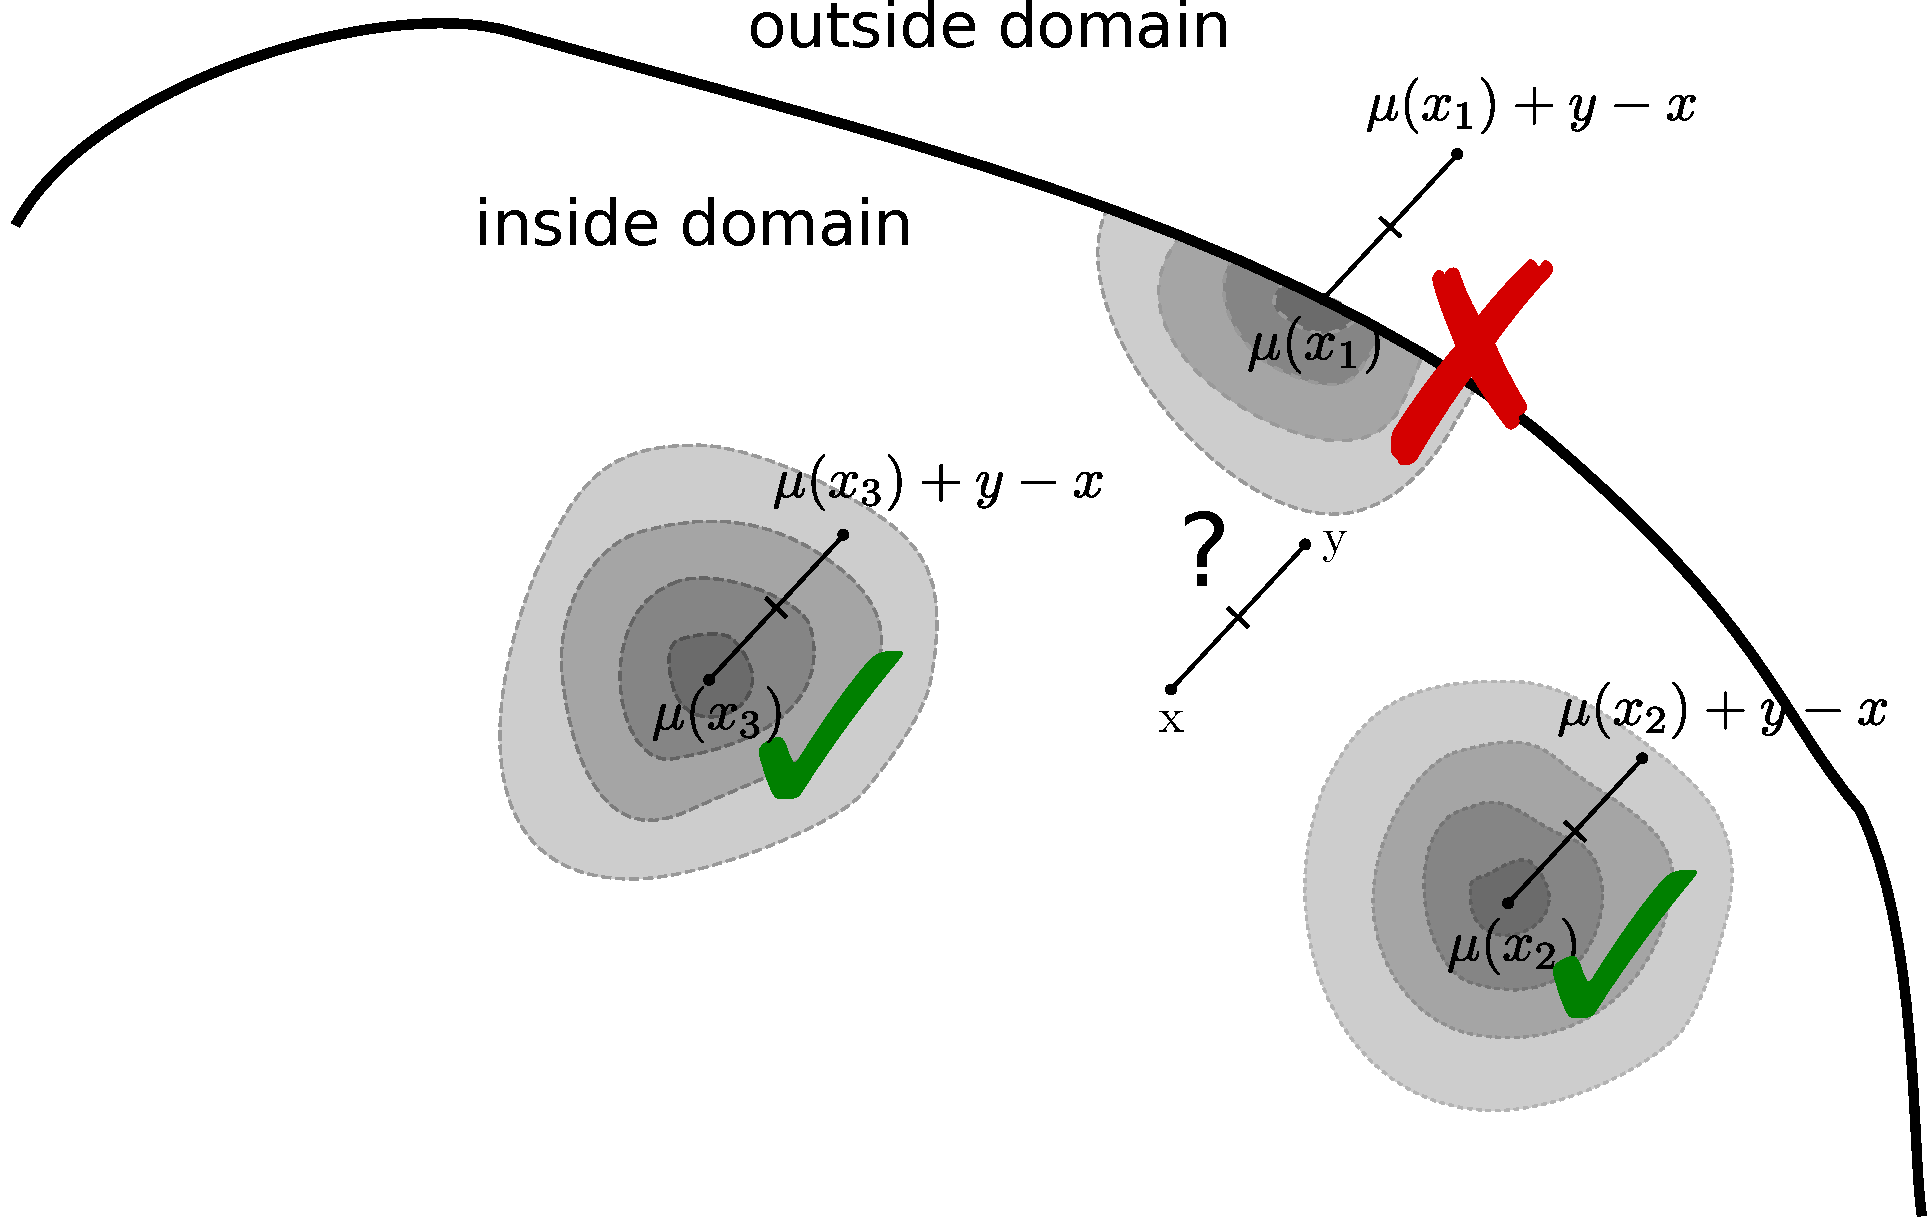
\includegraphics[scale=0.2]{interpolation_rbf_boundary.pdf}
%	\caption{To compute the kernel entry $\Aker(y,x)$, we use radial basis functions to interpolate the values $\frac{\spatialvol(x)}{\spatialvol(x_i)}\phi_{x_i}(y-\spatialmean(x)-\spatialmean(x_i))$ for the $\numnbr$ nearest sample points $x_i$ to $x$, excluding sample points for which $y-\spatialmean(x)-\spatialmean(x_i)$ is outside of the domain.}
%	\label{fig:rbf_interpolation}
%\end{figure}

To evaluate $f_i$, we check whether $z_i \in E_{x_i}$ using~\eqref{eq:support_ellipsoid}. If $z_i \notin E_{x_i}$, then $z_i$ is outside the estimated support of $\impulseresponse_{x_i}$, so we set $f_i=0$. If $z_i \in E_{x_i}$, we look up the batch index $b$ such that $x_i \in S_b$, and evaluate $f_i$ via the formula
$
f_i = \spatialvol(x)\eta_b\left(z_i\right),
$
per~\eqref{eq:varphi_eval}. Note that $z_i$ is typically not a gridpoint of the mesh used to discretize the problem, even if $y$, $x$, and $x_i$ are gridpoints. Hence,
evaluating $\eta_b\left(z_i\right)$ requires determining which mesh cell contains $z_i$, then evaluating finite element basis functions on that mesh cell. Fortunately, the mesh cell containing $z_i$ was determined as a side effect of querying the AABB tree of mesh cells when we checked whether $z_i \in \Omega$. 



\subsection{Hierarchical matrix construction}
\label{sec:h_matrix_construction_short}

We form our H-matrix approximation $\mathbf{A}_H \approx \mathbf{A}$ by forming H-matrix representations $\mathbf{\Aker}_H$ and $\massmatrix_H$ of $\mathbf{\Aker}$ and $\massmatrix$, respectively, then using fast H-matrix methods to multiply these matrices per~\eqref{eq:boldA} to form
$
\mathbf{A}_H = \massmatrix_H \mathbf{\Aker}_H \massmatrix_H.
$
%Once $\mathbf{A}_H$ is formed, useful matrix operations such as matrix-vector products, matrix-matrix addition, matrix-matrix multiplication, and matrix inversion may be performed using fast scalable H-matrix methods~\cite{BORMHACKBUSCHBOOK}. 
We use H1 matrices in our numerical results, but any other H-matrix format could be used instead. For more details on H-matrices, see~\cite{Hackbusch15}. 

We form $\mathbf{\Aker}_H$ using the standard geometrical clustering/adaptive cross method implemented within the HLIBpro software package~\cite{Kriemann08}. For details about the algorithms used for geometrical clustering, H-matrix construction, and H-matrix operations in HLIBpro, we recommend the the following papers~\cite{BormGrasedyckHackbusch03,GrasedyckKriemannLeBorne08,Kriemann13}. Although $\mathbf{\Aker}$ is a dense $\fedim \times \fedim$ matrix, constructing $\mathbf{\Aker}_H$ only requires evaluation of $O(\hrank^2 \fedim \log \fedim)$ kernel entries $\mathbf{\Aker}_{ij} = \widetilde{\Aker}(\fepoint_i, \fepoint_j)$, and these entries are computed via the radial basis function interpolation method described in Section~\ref{sec:approximate_kernel_entries}. Here $\hrank$ is the rank of the highest rank block in the H-matrix. 
A dense representation of $\mathbf{\Aker}$ is never formed. 
%We describe this H-matrix construction process in detail in Appendix~\ref{app:h_matrix}. 
We form $\massmatrix_H$ using standard H-matrix methods for sparse matrices implemented within HLIBpro, using the same geometrical clustering block cluster tree as was used for $\mathbf{\Aker}$. 



\section{Computational cost}
\label{sec:overall_cost}

The computational cost of our method may be divided into the costs to perform the following tasks: (1) Computing impulse moments and batches; (2) Building the H-matrix; (3) Performing linear algebra operations with the H-matrix. This may optionally include modifying the H-matrix to make it symmetric positive semi-definite.
In practice, (1) is the dominant cost, because (1) is the only task that requires applying $\Aop$ to vectors, and our method is targeted at applications in which applying $\Aop$ to a vector requires an expensive computational procedure such as solving a large scale PDE. All operations that do not require applications of $\Aop$ to vectors are nearly linear, and therefore scalable, in the size of the problem, $N$.
We now describe these costs in detail. For convenience, Table~\ref{tab:vars} lists variable symbols and their approximate sizes.

\begin{table}
	\begin{tabular}{lll}
		Symbol & Typical size & Variable name \\
		\hline
		$\fedim$ & $10^2$--$10^9$ & Number of finite element degrees of freedom \\
		$\nbatch$ & $1$--$25$ & Number of batches \\
		$\hrank$ & $5$--$50$ & H-matrix rank \\
		$\numnbr$ & $5$--$15$ & Number of nearest neighbors for RBF interpolation \\
		$\gdim$ & $1$--$3$ & Spatial dimension \\
%		$\classicalrank$ & $10^1$--$10^4$ & Classical matrix rank \\
		$\nsamplepts$ & $10^1$--$10^4$ & Total number of sample points (all batches) \\
		$|\pointbatch_i|$ & $1$--$500$ & Number of sample points in the $i$th batch \\
		$\ratord$ & $1$--$2$ & Rational function parameter for SPSD modification
	\end{tabular}
	\caption{Symbols used for variables in computational cost estimates, and approximate ranges for their sizes in practice.}
	\label{tab:vars}
\end{table}

\paragraph{(1) Computing impulse response moments and batches} Computing $\spatialvol$, $\spatialmean$, and $\spatialcov$ requires applying $\Aop$ to $1$, $\gdim$, and $\gdim(\gdim+1)/2$ vectors, respectively.
Computing each $\eta_i$ requires applying $\Aop$ to one vector, so computing $\{\eta_i\}_{i=1}^{\nbatch}$ requires $\nbatch$ operator applies. In total, computing all impulse response moments and batches therefore requires
\begin{equation*}
	1 + \gdim + \gdim(\gdim+1)/2 + \nbatch \qquad \text{operator applies.}
\end{equation*}
In a typical application one might have $\gdim=2$ and $\nbatch=5$, in which case a modest $11$ operator applies are required.

Computing the impulse response batches also requires choosing sample point batches via the greedy ellipsoid packing algorithm described in Section~\ref{sec:sample_point_selection}. Choosing the $i$th batch of sample points may require performing up to $\fedim |\pointbatch_i|$ ellipsoid intersection tests, where $|\pointbatch_i|$ is the number of sample points in the $i$th batch. Choosing all of the sample points therefore requires performing at most
\begin{equation*}
	\fedim \nsamplepts \qquad \text{ellipsoid intersection tests,}
\end{equation*}
where $\nsamplepts$ is the total number of sample points in all batches. The multiplicative dependence of $\fedim$ with $\nsamplepts$ is undesirable since $\nsamplepts$ may be large, and reducing this cost is a target for future work. 
%Several improvements are possible. The cost of picking sample points could be reduced by ``thinning'' the set of candidate points that the sample points are picked from. That is, choosing sample points from a smaller subset of $\fedim_\text{thin} << \fedim$ points. The cost to perform the ellipsoid intersection tests could be reduced by first checking whether the ellipsoid bounding boxes intersect before performing the ellipsoid intersection test of Appendix~\ref{sec:fast_ellipsoid_intersection_test}. The cost of picking the $i$th batch could be reduced to $O(\fedim \log |\pointbatch_i|)$ using more advanced computational geometry techniques, such as organizing the ellipsoids associated with points that have already been picked into a dynamic AABB tree, then using this AABB tree to accelerate the required ellipsoid intersection tests. 
However, from a practical perspective, the cost for picking sample points is small compared to other parts of the approximation algorithm, so we do not pursue these improvements in this paper.

\paragraph{(2) Building the H-matrix} The classical H-matrix construction technique
%, which is described in Appendix~\ref{app:h_matrix}, 
requires evaluating $O(\hrank^2 \fedim \log \fedim)$ matrix entries of the approximation, where $\hrank$ is the H-matrix rank, i.e,  the maximum rank among the blocks of the H-matrix. To evaluate one matrix entry, first one must find the $\numnbr$ nearest sample points to a given point, where $\numnbr$ is the number of impulse responses used in the RBF interpolation. This is done using a precomputed kd-tree of sample points, and requires $O(\numnbr \log \nsamplepts)$ floating point and logical elementary operations. Second, one must find the mesh cells that the points $\{z_i\}_{i=1}^{\numnbr}$ reside. This is done using an AABB tree of mesh cells, and requires $O(\numnbr \log \fedim)$ elementary operations. Third, one must evaluate finite element basis functions on each of those cells, which requires $O(\numnbr)$ elementary operations. Finally, one must solve a $\numnbr \times \numnbr$ linear system to perform the radial basis function interpolation, which requires $O(\numnbr^3)$ elementary operations, which typically is negligible. Therefore, building the H-matrix requires
\begin{equation*}
	O\left(\left(\hrank^2 \fedim \log \fedim\right)\left(\numnbr \log \fedim + \numnbr^3\right)\right) \qquad \text{elementary operations}.
\end{equation*}
%This follows from the above discussion, and the fact that $\fedim \ge \nsamplepts$.

\paragraph{(3) Performing linear algebra operations with the H-matrix} It is well known that H-matrix methods for matrix-vector products, matrix-matrix addition, matrix-matrix multiplication, matrix factorization, and matrix inversion, and low rank updates require
\begin{equation}
\label{eq:H_matrix_cost_operations}
	O(\hrank^2 \fedim \log(\fedim)^a) \qquad \text{elementary operations},
\end{equation}
where $a \in \{0,1,2,3\}$~\cite{GrasedyckHackbusch03}. The precise cost depends on the type of H-matrix used and the operation being performed. In the numerical results (Section~\ref{sec:numerical_results}), we use one matrix-matrix addition to add the H-matrix approximation of the data misfit term in the Hessian to the regularization term in the Hessian. Constructing an H-matrix representation of the regularization term in the Hessian requires one matrix inversion and two matrix-matrix multiplications. Then, we use one matrix factorization to form a preconditioner for the Newton linear system. 
%We perform low-rank updates to the H-matrix as the Newton iterations proceed, as per the discussion in Appendix~\ref{sec:recycle_krylov}.
The rational method for modifying $\mathbf{A}_H$ to be positive semi-definite, described in Appendix~\ref{sec:make_spd}, is performed using two matrix-matrix additions, $\ratord+1$ matrix-matrix multiplications, and one matrix inversion, where $2^\ratord$ is the rational function order.


\section{Numerical results}
\label{sec:numerical_results}


We use our method to approximate the Newton (or Gauss-Newton) Hessian
in inverse problems governed by PDEs which model steady state ice
sheet flow~\cite{PetraEtAl12} (Section~\ref{sec:ice}) and transport
and flow of a contaminant~\cite{PetraStadler11}
(Section~\ref{sec:adv}). 
To reconstruct the unknown parameter fields, denoted $q$, the inverse problems are formulated as nonlinear least squares
optimization problems, whose cost functions consist of a misfit term
(between the observations and model output) and a bi-Laplacian
regularization term following~\cite{VillaPetraGhattas21}. The
regularization is centered at a constant function $q_0(x)$. To
mitigate boundary effects
%For stokes q_0(x) = 10.5$%
we use a constant coefficient Robin boundary condition as
in~\cite{Roininen14}. The parameters for the regularization are chosen
so that the Green's function of the Hessian of the regularization has
a characteristic length of $0.25$ (NOTE: CHECK THIS FOR BOTH PROBLEMS) of the domain radius. For the
specific setup, we refer the reader to~\cite[Section
  2.2]{VillaPetraGhattas21}. For both examples, we choose the
regularization parameter, $\gamma$, that controls the overall strength
of the regularization using Morozov's discrepancy
principle~\cite{Vogel02}. The optimal value of $\gamma$ is used for
%  $\gamma =  7.3 \times 10^3$ for Stokes  Figure~\ref{fig:gamma_sweep}
all the numerical results except for the studies where we study how
changing $\gamma$ impacts the effectiveness of the proposed
preconditioner.

We solve the ice sheet inverse problem with an inexact Newton preconditioned
conjugate gradient (PCG) scheme and a globalizing Armijo line search~\cite{NocedalWright99}. The Newton updates,
$\bm{\searchdir}_k$, are obtained by solving 
%
\begin{equation}
	\label{eq:newton_system}
	\bm{H} \bm{\searchdir}_k = - \bm{g}_k \qquad \text{or} \qquad \bm{H}_\text{gn} \bm{\searchdir}_k = - \bm{g}_k,
\end{equation}
%
wherein we choose the initial guess as the discretization of the constant
function $q_0$. Here $\bm{g}_k$, $\bm{H}$ and $\bm{H}_\text{gn}$ are
the discretized gradient, Hessian, and Gauss-Newton Hessian of the
inverse problem cost function, respectively.
%The Gauss-Newton Hessian is Hessian of $J$, except in the data misfit, $J_d$, the nonlinear mapping $\basalfriction \mapsto \tangentop \velocity$ is replaced by its local linearization at $\basalfriction_k$.
To ensure positive definiteness of the Hessian we use
$\bm{H}_\text{gn}$ for the first five iterations, and $\bm{H}$ for all
subsequent iterations. The Newton iterations are terminated when
$||\bm{g}_k||/||\bm{g}_0|| < 10^{-8}$. Systems~\eqref{eq:newton_system} are solved inexactly using an inner PCG
iteration, which terminates when the norm of the linear system residual is less than $\min \left(0.5,
\sqrt{||\bm{g}_k||}\right)||\bm{g}_k||$. The advection-diffusion inverse problem is linear, so Newton's method converges in one iteration. In this case the Newton linear system,~\eqref{eq:newton_system}, is solved using PCG with a fixed tolerance which is specified in Section~\ref{sec:adv}.

We use the framework described in this paper to generate Hessian preconditioners. We build H-matrix approximations, $\mathbf{A}_H$, of the data misfit Gauss-Newton Hessian (the term in $\bm{H}_\text{gn}$ that arises from the data misfit). The 
%number of impulse response batches used to build these 
approximations are indicated by ``PSF ($\nbatch$)'', where $\nbatch$ is the number of impulse response batches used to build the approximation. The Hessian of the regularization term is a combination of
stiffness and mass matrices, which are sparse. Therefore, we form
H-matrix representations of these matrices and combine them into a H-matrix approximation of the regularization term in the Hessian, $\mathbf{R}_H$, using
standard sparse H-matrix techniques. H-matrix approximations of the Gauss-Newton Hessian, 
$$\bm{H}_\text{gn}\approx \widetilde{\mathbf{H}}:=\mathbf{A}_H + \mathbf{R}_H,$$
are formed by adding $\bm{A}_H$ to $\mathbf{R}_H$ using fast H-matrix arithmetic. The H-matrix $\widetilde{\mathbf{H}}$ may be indefinite due to approximation error, so we modify it to be symmetric positive definite via a shift and invert deflation procedure described in Appendix~\ref{sec:make_spd}. We factor $\bm{\preconditioner}$,
using fast H-matrix methods, then use the factorization as a
preconditioner. We approximate $\bm{H}_\text{gn}$ rather than $\bm{H}$ because $\bm{H}$ more often has negative values in its integral kernel. Our results show that $\widetilde{\mathbf{H}}$ is a good preconditioner for both $\bm{H}_\text{gn}$ and $\bm{H}$. 
%The H-matrix approximation of the data misfit Gauss-Newton Hessian is added to an H-matrix approximation of the Hessian of the regularization term to form an H-matrix approximation of $\bm{H}_\text{gn}$.
%
%Straightforward calculation shows that the discretized Hessian of the regularization term is given by
%$
%(\gamma \bm{K} + \delta \bm{M}) \bm{M}^{-1} (\gamma \bm{K} + \delta \bm{M})
%$
%where $\bm{K}$ is a finite element stiffness matrix with appropriate boundary conditions, and $\bm{M}$ is the finite element mass matrix. These matrices are sparse, so we form H-matrix representations of these matrices and combine them using standard sparse H-matrix techniques.
%



\subsection{Example 1: Inversion for the basal sliding coefficient in an ice sheet flow problem}
\label{sec:ice}

%\textbf{Heat equation}
%\begin{itemize}
%	\item Hessian per-column error plots for 1, 5, and 15 batches
%	\item $H-P$ error vs number of batches for interior and whole domain
%	\item $P^{-1}H-I$: error vs rank for $P=R$ and $P=P_\text{pch}$ diffusion time, for 1, 5, and 15 batches
%	\item Krylov iterations to tols 1e-1 and 1e-6 vs diffusion parameter
%	\item GLR vs PCH vs diffusion time
%	\item Krylov method convergence plot: $R$ vs $P_\text{pch}$ vs no preconditioner
%	\item Krylov iterations to tols 1e-6 vs mesh size $h$, PCH vs R vs no preconditioner (hold)
%	\item true parameter (H)
%	\item deterministic reconstruction (H)
%	\item noisy measurements (1\%, 5\%, 10\% noise). $u|_\text{top}$ (H)
%	\item recovered state at top (H)
%	\item mesh scalability of PCH (CC) (H)
%	\item put plot data into data directory
%	\item save function .pvd files in paraview  directory
%\end{itemize}
%
%\begin{itemize}
%	\item GLR vs PCH number of obs (Computational cost in PDE solves) (S)
%	\item GLR vs PCH aspect ratio (CC) (S)
%	\item turn on preconditioner after number of krylov iterations exceeds 15 in an iteration. Rebuild "as needed". (S)
%\end{itemize}
%
%\begin{itemize}
%	\item Stokes Krylov convergence (10 solves for nonlinear forward + 6 hessian matvecs for ellipsoid estimation + 10 matvecs for impulse responses + 30 matvecs for PCH6 CG solve + 100 matvecs for Reg CG solve)
%	\item Stokes error vs num batches (small number of batches; 1, 3, 6, 9 batches?) (50 matvecs for randomized error estimation +)
%	\item Velocity field
%	\item basal sliding field
%	\item Picture of impulse responses
%	\item Mesh negative numbers picture
%\end{itemize}
%
%\begin{itemize}
%	\item mtrue
%	\item utrue (no arrows)
%	\item utrue (yes arrows)
%	\item reconstruction iterations 1,3,4,8: PCH vs REG
%	\item urecovered (arrows, 3D)
%	\item morozov plot
%	\item Newton convergence (iter, numcg, numPDEsolves (num preconditioner build), gradnorm)
%	\item impulse response batches
%	\item 
%\end{itemize}

For this example, we consider a sheet of ice flowing down a mountain (see Figure~\ref{fig:ice_mountain_mesh}). Given observations of the tangential component of the ice velocity on the top surface of the ice, we invert for the logarithm of the unknown spatially varying basal sliding Robin coefficient field, which governs the resistance to sliding along the base of the ice sheet. %The inverse problem considered here is synthetic, but in practice surface velocity observations are available from satellites.
%
%
\begin{figure}
	\begin{center} 
	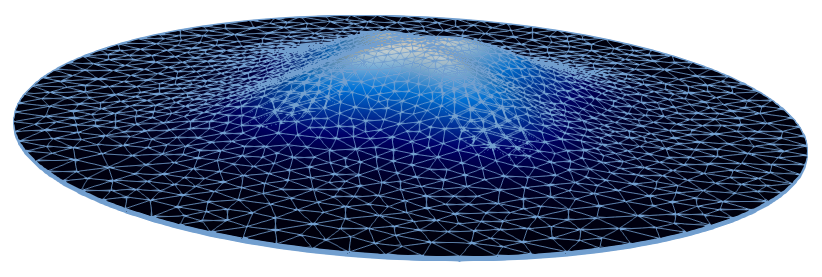
\includegraphics[scale=0.23]{meshHeight_view2_edges.png}
	\end{center}
	\caption{Bird's eye view of the ice sheet, discretized by a mesh of tetrahedra. Color indicates the height of the base of the ice sheet (i.e., the mountain topography). The radius of the domain is $10^4$ meters, the maximum height of the mountain is $2.1 \times 10^3$ meters, and the average thickness of the ice sheet is 250 meters.}
	\label{fig:ice_mountain_mesh}
\end{figure} 
%
%
The domain that is filled with ice is denoted by
$\icedomain \subset\mathbb{R}^{3}$. The basal, lateral and top parts of $\partial \icedomain$ are denoted by $\Gamma_{b}$, $\Gamma_{l}$, and $\Gamma_{t}$, respectively.
The governing equations are the linear incompressible Stokes
equations,
%
%
\begin{subequations}\label{Stokeseqn}
	\begin{align}
	%-\nabla \cdot \stress(v, p)
	%&=\bodyforce \,\,\,\,\,\text{ in }\icedomain, \label{Stokeseqn:1}\\
	%\nabla\cdot \velocity
	  %&=0\,\,\,\,\,\,\text{ in }\icedomain, \label{Stokeseqn:2}\\
          -\nabla \cdot \stress(v, p)=\bodyforce \text{ and }
          \nabla\cdot \velocity &=0 \quad \text{ in }\icedomain, \label{Stokeseqn:1}\\
	\stress(v, p)\normalvec
	&=0\,\,\,\,\,\,\text{ on }\Gamma_{t}, \label{Stokeseqn:3}\\
	\velocity \cdot\normalvec =0 \text{ and } \tangentop\left(\stress(v, p)\normalvec+\exp\left(\basalfriction\right)\velocity\right)
	&=0\,\,\,\,\,\,\text{ on }\Gamma_{b},\label{Stokeseqn:4} \\
	\stress(v, p)\normalvec+\stokesrobincoeff \velocity &=0\,\,\,\,\,\,\text{ on }\Gamma_{l}.\label{Stokeseqn:5}	
	\end{align}
\end{subequations}
The solution to these equations is the pair $(\velocity, \pressure)$, where $\velocity$ is the ice flow velocity field, and $\pressure$ is the pressure field. Here, $\basalfriction$ is the unknown logarithmic
basal sliding field (note that large $\basalfriction$ corresponds to high resistance to sliding) which is defined on the $2$D surface $\Gamma_b$. The quantity $\bodyforce$ is the body force density due to gravity, $\stokesrobincoeff=10^6$ is a Robin boundary condition constant,  $\normalvec$ is the outward normal and $\tangentop$ is the tangential projection operator that restricts a vector field to its tangential component along the boundary. 
We employ Glen's flow law~\cite{Glen1955}, $\stress(v, p)= 2\eta
\dot{\strain}(v) -I\pressure$,
which is a constitutive law for ice that relates the stress
tensor, $\stress$, to the strain rate tensor,
$\dot{\strain}(v)= \frac{1}{2}\left(
\nabla\velocity+\nabla\velocity^{\top} \right)$. Here $\eta$ is the effective viscosity and $I$ is the unit matrix. Glen's exponent has been chosen to be one, which provides for a linear Stokes model. Note that while the PDE is linear, the parameter-to-solution map, $\basalfriction \mapsto (\velocity, \pressure)$, is nonlinear.

The pressure, $\pressure$, is discretized with first order scalar continuous Galerkin finite elements defined on a mesh of tetrahedra. The velocity, $\velocity$, is discretized with second order continuous Galerkin finite elements on the same mesh. The parameter $\basalfriction$ is discretized with first order scalar continuous Galerkin finite elements on the mesh of triangles that results from restricting the tetrahedral mesh to the basal boundary, $\Gamma_b$. Note that $\Gamma_b$ is a 2D surface embedded in 3D due to the mountain topography. We also generate a flattened version of $\Gamma_b$, denoted by $\Omega \subset \mathbb{R}^2$, by ignoring the height coordinate. The parameter $\basalfriction$ is dually viewed as a function on $\Gamma_b$ for the purpose of solving the Stokes equations, and as a function on $\Omega$ for the purpose of building our Hessian approximations and defining the regularization. 
%This flattening is necessary because our operator approximation method requires adding points on this surface together to get other points on the surface, and this is only well-defined in flat space. 
The observations are generated by adding $1\%$ multiplicative
Gaussian noise to the tangential component of the velocity field
restricted to the top surface of the geometry. The true basal sliding
coefficient field and the true velocity field, which is obtained by
solving~\eqref{Stokeseqn}, are shown in Figure~\ref{fig:true_beta_u}.

\begin{figure}
	\begin{subfigure}{0.49\textwidth}
		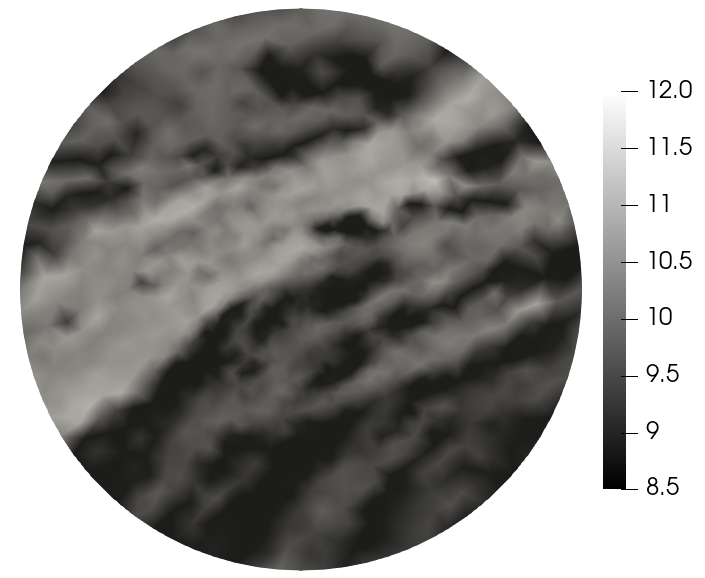
\includegraphics[scale=0.243]{mtrue_withColorBar.png}
		\caption{$\basalfriction_\text{true}$.}
	\end{subfigure}
	\begin{subfigure}{0.49\textwidth}
		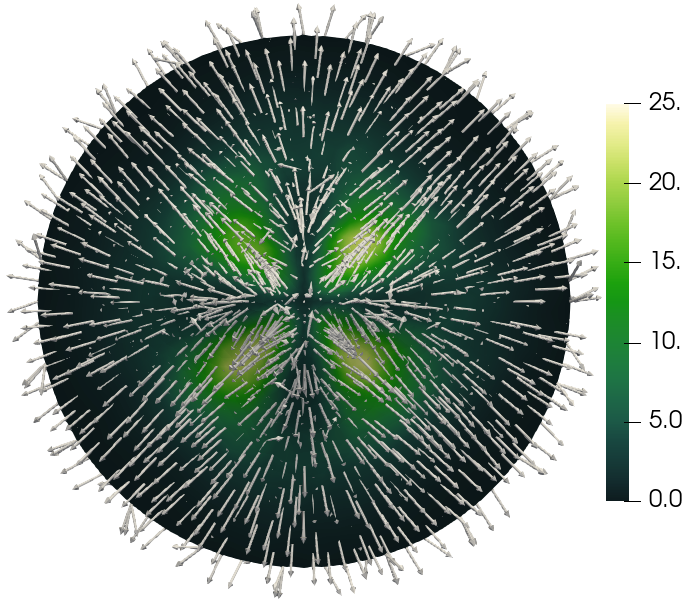
\includegraphics[scale=0.243]{trueVelocity2_glyphs.png}
		\caption{$\velocity_\text{true}$.}
	\end{subfigure}
	\caption{True parameter, $\basalfriction_\text{true}$, (left) and true velocity $\velocity_\text{true}$ (right). In the right plot, arrows indicate the direction of $\velocity_\text{true}$ and color indicates the magnitude of $\velocity_\text{true}$.}
	\label{fig:true_beta_u}
\end{figure} 

%aaa


%% from here we summarize --------
%The true parameter field, $\basalfriction_\text{true}$, and corresponding velocity field, $\velocity_\text{true}$, are shown in Figure~\ref{fig:true_beta_u}. We generate synthetic observations by restricting the tangential component of $\velocity_\text{true}$ to the top surface to get
%\begin{equation*}
%\observations_\text{true} = \tangentop \velocity_\text{true} |_{\Gamma_t}.
%\end{equation*}
%We add $1\%$ multiplicative Gaussian noise to all components of the finite element vector, $\bm{\observations}_\text{true}$, corresponding to the function $\observations_\text{true}$, which yields noisy synthetic observations, $\observations_\text{obs}$ which are used for the inversion. That is, 
%\begin{equation*}
%\left(\bm{\observations}_\text{obs}\right)_j := \left(\bm{\observations}_\text{true}\right)_j + 0.01 \cdot \boldsymbol{\xi}_j \cdot \left|\left(\bm{\observations}_\text{true}\right)_j\right|,
%\end{equation*}
%where $j$ ranges over all entries of the vector of coefficients representing the finite element functions $\observations_\text{true}$ and $\observations_\text{obs}$, and $\boldsymbol{\xi}_j$ are independent and identically distributed (i.i.d) random numbers drawn from the standard normal distribution. We also define the noise function, $\xi$, to be the finite element function with $j$th vector entry $\boldsymbol{\xi}_j$.
%
%The reconstructed parameter field $\basalfriction$ is found as the solution to an optimization problem of the following form:
%\begin{equation}
%	\label{eq:deterministic_optimization_problem}
%	\min_{\basalfriction} \quad J(\basalfriction) := J_d(\basalfriction) + J_r(\basalfriction).
%\end{equation}
%The first term in the objective function is
%\begin{equation*}
%	J_d(\basalfriction) := \frac{1}{2}\int_{\Gamma_{t}}||\observations_\text{obs} - \tangentop\velocity||_{2}^{2}\,dS.
%\end{equation*}
%We call this term the data misfit, because it measures the difference between the observed data and the predicted data based on a candidate parameter $\basalfriction$. Here $\velocity = \velocity(\basalfriction)$ denotes the velocity field solving $\ref{Stokeseqn}$ for the given parameter $\basalfriction$. The second term,
%\begin{equation*}
%	J_r(\basalfriction) := \frac{1}{2}\int_{\Omega}\left| \mathcal{K}(\basalfriction - \basalfriction_0)\right|^2\,dx,
%\end{equation*}
%is a Bilaplacian regularization term. Specifically, $\basalfriction_0$ is the constant function $\basalfriction_0(x)=10.5$, and $\mathcal{K}$ is the inverse of the solution operator for the following elliptic PDE:
%\begin{align*}
%-\gamma\Delta u +\delta\,u&=\regrhs\,\,\,\,\text{ in }\Omega,\\
%\gamma \nabla u\cdot\normalvec+\regrobincoeff\,u&=0\,\,\,\text{ on }\partial\Omega.
%\end{align*}
%Recall that $\Omega$ is the 2D flattened version of the basal surface $\Gamma_b$. Here $\regrhs$ is a generic forcing term, and $\regrobincoeff=\sqrt{\delta \gamma}/1.42$ is a Robin boundary condition coefficient~\cite{Roininen14}, and these quantities are different from $\bodyforce$ and $\stokesrobincoeff$ in the Stokes equation,~\eqref{Stokeseqn}.
%In all results except one, $\gamma$ is chosen so that the Morozov discrepancy principle is satisfied, i.e.,
%\begin{equation*}
%	\int_{\Gamma_{t}}||\observations_\text{obs} - \tangentop\velocity||_{2}^{2}\,dS = \int_{\Gamma_{t}}||\xi||_{2}^{2}\,dS.
%\end{equation*}
%The value of $\gamma$ satisfying the Morozov discrepancy principle is $\gamma=7.3 \times 10^3$. The exception is Figure~\ref{fig:gamma_sweep}, where we vary $\gamma$ to study how changing $\gamma$ impacts the effectiveness of our preconditioner. The constant $\delta$ is chosen so that the correlation length of functions drawn from the normal distribution with covariance $\mathcal{K}^{-2}$, given by $L=\sqrt{\gamma/\delta}$, is $1/10$th the radius of the domain. 
%%, which is halfway between the maximum and minimum values of $\basalfriction_\text{true}$.
%
%PCG only requires applying
%$\bm{H}$ (or $\bm{H}_\text{gn}$) to vectors. Each application of
%$\bm{H}$ (or $\bm{H}_\text{gn}$) to a vector requires solving one
%incremental forward and one incremental adjoint Stokes PDE of the form
%\eqref{Stokeseqn}, but with different right hand sides.
\begin{figure}
	\begin{subfigure}{0.24\textwidth}
		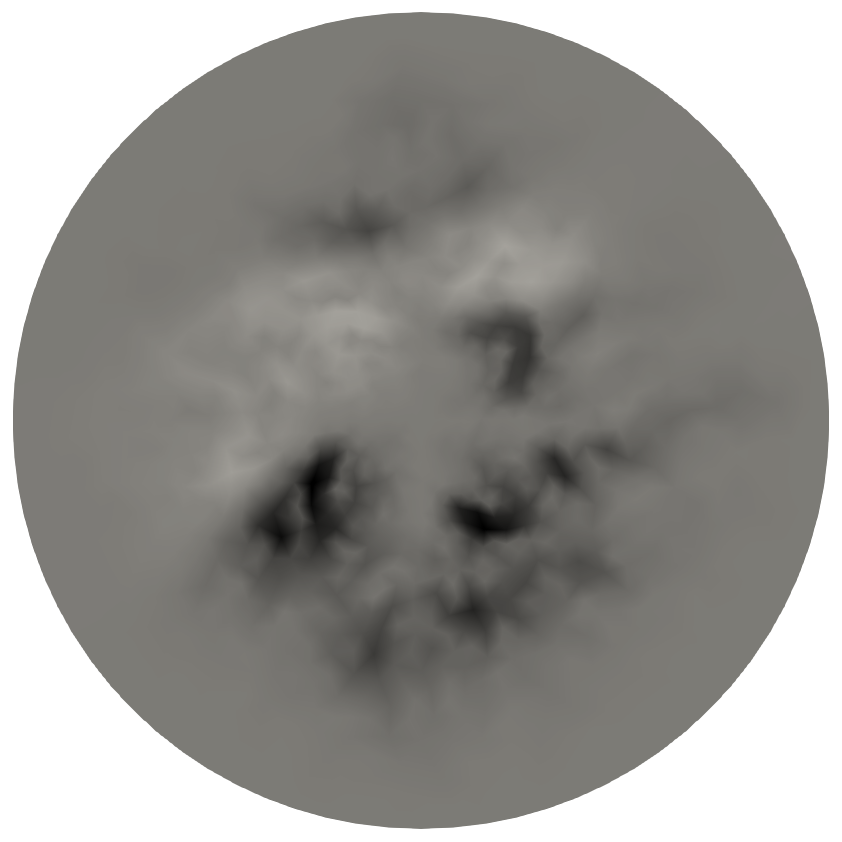
\includegraphics[scale=0.1]{m1_psf.png}
		%		\caption{}
		%		\label{fig:newtoniter1}
	\end{subfigure}
	\begin{subfigure}{0.24\textwidth}
		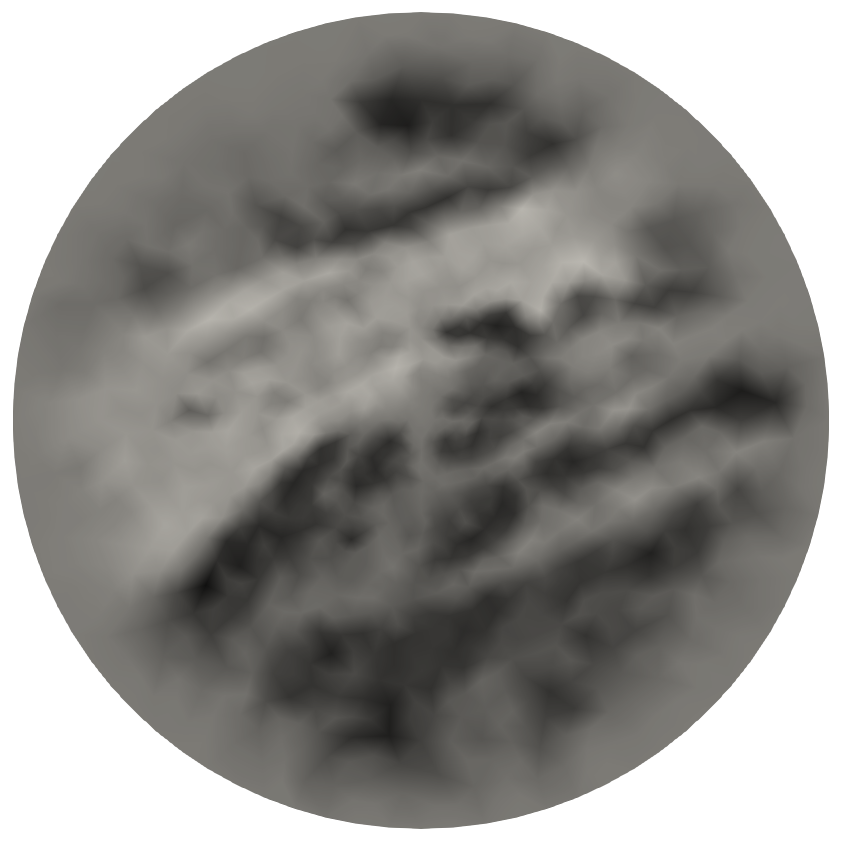
\includegraphics[scale=0.1]{m3_psf.png}
		%		\caption{}
		%		\label{fig:newtoniter2}
	\end{subfigure}
	\begin{subfigure}{0.24\textwidth}
		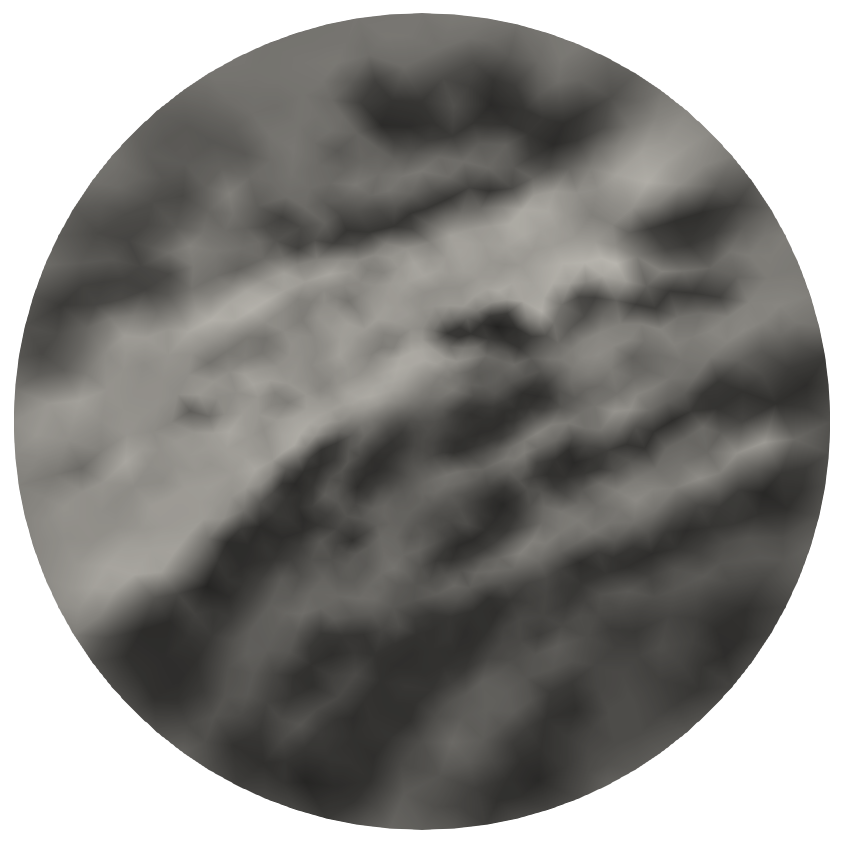
\includegraphics[scale=0.1]{m4_psf.png}
		%		\caption{}
		%		\label{fig:newtoniter3}
	\end{subfigure}
	\begin{subfigure}{0.24\textwidth}
		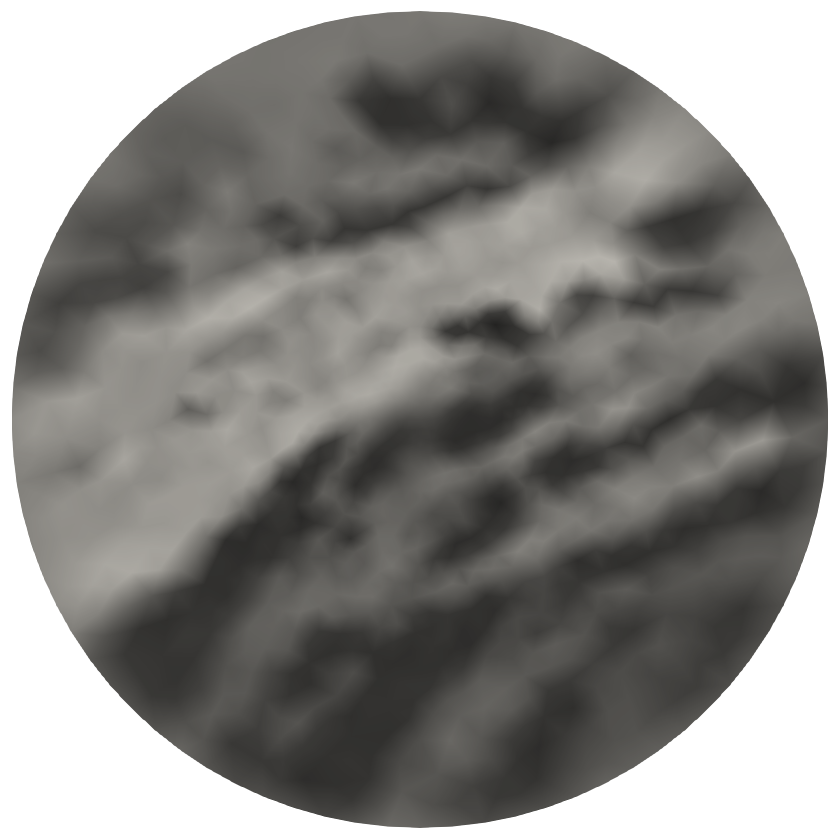
\includegraphics[scale=0.1]{m6_psf.png}
		%		\caption{}
		%		\label{fig:newtoniter4}
	\end{subfigure}
	%\begin{subfigure}{0.05\textwidth}
	%	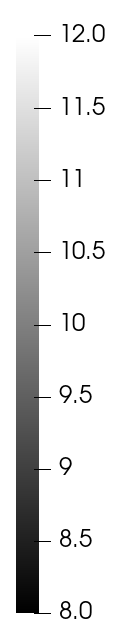
\includegraphics[scale=0.1]{mColorBar.png}
	%\end{subfigure}
	\caption{The log basal sliding parameter after $1$ (left), $3$ (second from left), and $4$ (third from left) Newton iterations, and the final Newton iterate (right). The PSF (5) preconditioner is constructed between Newton iterations 3 and 4.}
	\label{fig:newton_iterates} 
\end{figure} 

\begin{table}
	{\small
		\begin{center}
			\begingroup
			\setlength{\tabcolsep}{3pt}
			\renewcommand{\arraystretch}{1.1}
			\begin{tabular}{c| c c c | c c c | c c c}
				&  \multicolumn{3}{|c|}{PSF (5)} & \multicolumn{3}{|c|}{REG} & \multicolumn{3}{|c}{NONE} \\
				\hline
				Iter & 
				\#CG & \#Stokes & $||\bm{g}||$ & 
				\#CG & \#Stokes & $||\bm{g}||$ & 
				\#CG & \#Stokes & $||\bm{g}||$ \\
				0 &
				1 & 4 & 2.0e+7 &
				1 & 4 & 2.0e+7 &
				1 & 4 & 2.0e+7 \\
				1 &
				2 & 6 & 5.8e+6 &
				2 & 6 & 7.9e+6 &
				2 & 6 & 5.8e+6 \\
				2 &
				4 & 10 & 2.4e+6 &
				5 & 12 & 3.9e+6 &
				4 & 10 & 2.4e+6 \\
				3 &
				2 & 6+22 & 5.8e+5 &
				13 & 28 & 1.6e+6 &
				13 & 28 & 5.8e+5 \\
				4 &
				5 & 12 & 5.6e+4 &
				42 & 86 & 4.8e+5 &
				33 & 68 & 9.1e+4 \\
				5 &
				10 & 22 & 3.5e+3 &
				84 & 170 & 7.7e+4 &
				57 & 116 & 6.2e+3 \\
				6 &
				14 & 30 & 2.7e+1 &
				125 & 252 & 5.0e+3 &
				76 & 154 & 1.1e+2 \\
				7 &
				0 & 2 & 4.1e-2 &
				194 & 390 & 7.9e+1 &
				117 & 236 & 2.3e-1 \\
				8 & 
				--- & --- & --- &
				0 & 2 & 1.6e-1 &
				0 & 2 & 4.1e-2 \\
				\hline
				Total & 
				38 & 114 & --- &
				466 & 950 & --- &
				303 & 624 & --- \\
			\end{tabular}
			\endgroup
		\end{center}
	}
	\caption{Convergence history for solving the Stokes inverse problem using preconditioned inexact Newton PCG. Preconditioners shown are our method with five batches (PSF (5)) constructed at the third iteration, regularization preconditioning (REG), and no preconditioning (NONE). Columns titled \#CG show the number of PCG iterations used to solve the Newton system for $\bm{\widehat{\basalfriction}}_k$. Columns titled $||\bm{g}||$ show the $l^2$ norm of the gradient at $\bm{\basalfriction}_k$. Columns titled \#Stokes show the total number of Stokes PDE solves performed in each Newton iteration. This consists of Stokes solves for $u$ performed during the linesearch going from $\bm{\basalfriction}_{k-1}$ to $\bm{\basalfriction}_k$, plus one adjoint Stokes solve to compute the gradient at $\bm{\basalfriction}_k$, plus one incremental forward and one incremental adjoint Stokes solve per PCG iteration for solving the Newton system. In the PSF (5) portion of row 3, we write $6+22$ to indicate that 6 Stokes solves were used during the standard course of the iteration, and 22 Stokes solves were used to build the PSF (5) preconditioner.}
	\label{tab:newton_convergence_table}
\end{table}

Table~\ref{tab:newton_convergence_table} shows the performance of our preconditioner for accelerating the solution of optimization problem~\eqref{eq:deterministic_optimization_problem}. We build the PSF (5) preconditioner in the third Gauss-Newton iteration, and reuse it for all subsequent Gauss-Newton and Newton iterations. No preconditioning is used in the Gauss-Newton iterations before the PSF (5) preconditioner is built. We compare our method with the most commonly used existing preconditioners: no preconditioning (NONE), and preconditioning by the regularization term in the Hessian (REG). Using PSF (5) reduces the total number of Stokes PDE solves by a factor of six compared to no preconditioning, and by a factor of nine compared to regularization preconditioning\footnote{Interestingly, we observe that no preconditioning outperforms regularization preconditioning here because the noise level (and hence $\gamma$) is small.}. In Figure~\ref{fig:newton_iterates} we show select Newton iterates using our PSF (5) preconditioner.
%
%
\begin{figure}
	\begin{subfigure}{0.49\textwidth}
		\centering
		\begin{tikzpicture}[baseline, trim axis right]
		\begin{axis}[width=0.99\linewidth, height=1.0\linewidth,
		ymode=log,
		ymin=1e-13,
		ymax=2,
		xmax=750,
		axis x line*=bottom,
		axis y line*=left,
		xtick={0, 200, 400, 600},
		title={CG convergence},
		xlabel={$k$, CG iteration},
		ylabel={$||\bm{x}_k-\bm{x}_{\text{true}}||/||\bm{x}_{\text{true}}||$},
		legend style={at={(1.1,1)},anchor=north east},
		%legend pos=north east,
		legend style={font=\small}
		]
		\addlegendentry{Reg}		
		\addplot[dotted, line width=0.5mm] table {cg_relres_reg_0.05noise.dat};
		\addlegendentry{None}
		\addplot[dash dot, line width=0.5mm] table {cg_relres_none_0.05noise.dat};
		\addlegendentry{PSF (1)}
		\addplot[blue, line width=0.5mm] table {cg_relres_psf1_0.05noise.dat};
		\addlegendentry{PSF (5)}
		\addplot[red, line width=0.5mm] table {cg_relres_psf5_0.05noise.dat};
		\addlegendentry{PSF (25)}
		\addplot[purple, line width=0.5mm] table {cg_relres_psf25_0.05noise.dat};
		\end{axis}
		\end{tikzpicture}
		\caption{}
		\label{fig:cg_convergence}
	\end{subfigure}
	\begin{subfigure}{0.49\textwidth}
	\begin{center}
		\begin{tikzpicture}[baseline, trim axis right]
		\begin{axis}[width=0.99\linewidth, height=1.0\linewidth,
		ymode=log,
		xmin=-50,
		xmax=1450,
		ymax=1.e7,
		title={Generalized eigenvalues, $\bm{H} \bm{u}_{k}=\lambda_{k} \bm{\preconditioner} \bm{u}_{k}$},
		xlabel={$k$, generalized eigenvalue \#},
		ylabel={$\lambda_{k}$},
		xtick={0, 300, 600, 900, 1200},
		%legend pos=north east,
		legend style={font=\small},
		ylabel near ticks, %ylabel shift={-6pt},
		axis x line*=bottom,
		axis y line*=right,
		%legend style={at={(0.95,1)},anchor=north east},
		]
		%\addlegendentry{REG}
		\addplot[dotted, line width=0.5mm] table[x=k, y=reg] {generalizedEigenvalues_0.05noise.dat};
		\addplot[dash dot, line width=0.5mm] table[x=k, y=none] {generalizedEigenvalues_0.05noise.dat};
		%\addlegendentry{PSF (1)}
		\addplot[blue, line width=0.5mm] table[x=k, y=psf1] {generalizedEigenvalues_0.05noise.dat};
		%\addlegendentry{PSF (5)}
		\addplot[red, line width=0.5mm] table[x=k, y=psf5] {generalizedEigenvalues_0.05noise.dat};
		%\addlegendentry{PSF (25)}
		\addplot[purple, line width=0.5mm] table[x=k, y=psf25] {generalizedEigenvalues_0.05noise.dat};
		\end{axis}
		\end{tikzpicture}
	\end{center}
	\caption{}
	\label{fig:generalized_eigenvalues}
    \end{subfigure}
	\caption{Left (\ref{fig:cg_convergence}) shows the convergence history for solving $\bm{H} \bm{x} = \bm{b}$ using PCG, where $\bm{b}$ has i.i.d. random entries drawn from the standard normal distribution. The reference solution $\bm{x}_{\text{true}}$ is determined by solving $\bm{H} \bm{x} = \bm{b}$ to an accuracy of ? using method ? (\todo{include details about $\bm{x}_{\text{true}}$ here}). 
	Here we use $\gamma=7.3 \times 10^3$, which is determined by the Morozov discrepancy principle. Results in these figures are shown for our preconditioner with 1, 5, and 25 batches (PSF (1), PSF (5), and PSF(25), respectively), regularization preconditioning (REG), and no preconditioning (NONE). The preconditioner is constructed using $\bm{H}_\text{gn}$.
	Right (\ref{fig:generalized_eigenvalues}): eigenvalues for generalized eigenvalue problem $\bm{H} \genericvec_k = \lambda_k \bm{\preconditioner} \genericvec_k$. Here $\bm{H}$ is the Hessian and $\bm{\preconditioner}$ is the PSF approximation constructed using the Gauss-Newton Hessian, $\bm{H}_\text{gn}$, for 1, 5, and 25 batches (PSF (1), PSF (5), and PSF (25), respectively), or the regularization Hessian (REG).}
	\label{fig:krylov_convergence}
\end{figure} 
%
%
Next, we build PSF (1), PSF (5), and PSF (25) preconditioners based on the Gauss-Newton Hessian evaluated at the converged solution $\bm{\basalfriction}$. We use PCG to solve a linear system with the Hessian as the coefficient operator and a right hand vector with random i.i.d. entries drawn from the standard normal distribution. In Figure~\ref{fig:cg_convergence} we compare the convergence of PCG for solving this linear system using the PSF (1), PSF (5), PSF (25), REG, and NONE preconditioners. PCG converges fastest with the PSF preconditioners, with PSF (25) converging fastest, followed by PSF (5), followed by PSF (1), as expected. PCG converges much slower with no preconditioning and regularization preconditioning than it does with PSF preconditioning, with no preconditioning outperforming regularization preconditioning. In Figure~\ref{fig:gamma_sweep}, we perform PCG solves on linear systems of the same form, except now we vary $\gamma$. The performance of our PSF preconditioners is good and relatively stable over a wide range of $\gamma$'s. All PSF preconditioners perform the same for medium and large values of $\gamma$. For small values of $\gamma$ PSF (25) performs slightly better than PSF (5), which performs slightly better than PSF (1). As expected, regularization preconditioning performs well for large $\gamma$ and poorly for small $\gamma$. Our PSF preconditioners outperform no preconditioning and regularization preconditioning for medium and small $\gamma$, and perform similarly to regularization preconditioning for large $\gamma$.

\begin{figure}
	\begin{center}
			\begingroup
			\setlength{\tabcolsep}{4pt}
			\renewcommand{\arraystretch}{1.25}
			\begin{tabular}{c| c c c c c}
				noise    & \multicolumn{5}{c}{COND$(\bm{\preconditioner}^{-1} \bm{H})$ } \\ \cline{2-6}
				level    & REG     &	NONE  & PSF $(1)$ & PSF $(5)$ & PSF $(25)$ \\ \hline 
				$25\%$   & 1.68e+3 & 2.16e+3  & 1.37e+0   & 1.30e+0   & 1.21e+0    \\ 
				$11\%$   & 9.19e+3 & 9.08e+2  & 1.85e+0   & 1.49e+0   & 1.27e+0    \\   
				$5.0\%$  & 3.66e+4 & 4.67e+2  & 3.46e+0   & 2.62e+0   & 1.91e+0    \\ 
				$2.2\%$  & 1.41e+5 & 8.25e+2  & 1.16e+1   & 4.99e+0   & 3.20e+0    \\  
				$1.0\%$  & 6.06e+5 & 1.70e+3  & 3.44e+1   & 5.38e+1   & 7.06e+0    \\   
			\end{tabular}
			\endgroup
		\end{center}
	\caption{Condition number for $\bm{\preconditioner}^{-1} \bm{H}$ for our preconditioner with 1, 5, and 25 batches (PSF (1), PSF (5), and PSF(25), respectively), no preconditioner (NONE) and regularization (REG). All operators are evaluated at the $\bm{\basalfriction}$ that solves the inverse problem for 
	the regularization value $\gamma$ as determined by noise level by means of the Morozov discrepancy principle.}
	\label{fig:condition_number}
\end{figure}

In Figure~\ref{fig:generalized_eigenvalues} we show the generalized eigenvalues for the generalized eigenvalue problem
$
	\bm{H} \genericvec = \lambda \bm{\preconditioner} \genericvec.
$
Here $\bm{H}$ is the Hessian evaluated at the reconstructed parameter $\bm{\basalfriction}$ for $\gamma$ chosen to satisfy the Morozov discrepancy principle. The matrix $\bm{\preconditioner}$ is one of the PSF (1), PSF (5), or PSF (25) Gauss-Newton Hessian approximations constructed at that $\bm{\basalfriction}$, or the regularization Hessian. The PSF preconditioners cluster the eigenvalues of the Hessian near one, with more batches yielding better clustering. The regularization preconditioner clusters the trailing eigenvalues but amplifies leading eigenvalues. In Figure~\ref{fig:condition_number} we show the condition numbers of $\bm{\preconditioner}^{-1} \bm{H}$ and $\bm{\preconditioner}^{-1} \bm{H}_\text{gn}$. The PSF preconditioners yield the the smallest condition numbers, with more batches yielding smaller condition numbers. Regularization preconditioning and no preconditioning yield larger condition numbers. The condition numbers are similar for both $\bm{\preconditioner}^{-1} \bm{H}$ and $\bm{\preconditioner}^{-1} \bm{H}_\text{gn}$, demonstrating that the preconditioner built based on $\bm{H}_\text{gn}$ is a good preconditioner for $\bm{H}$.


\subsection{Example 2: Inversion for the initial condition in an advection-diffusion problem}
\label{sec:adv}

Here we consider a time-dependent advection-diffusion equation for
which we seek to infer the unknown spatially varying initial condition, $\ipar$, from observations of the state  
at a final time. This PDE
models diffusive transport in a domain $\advdomain \subset \R^d$, which is
depicted in Figure~\ref{fig:adv_inversion1}. In this case, the state, $\concentration(x,t)$, could be interpreted as the concentration of a contaminant. The problem description
below closely follows the one in~\cite{PetraStadler11}. The domain
boundaries $\partial \advdomain$ include the outer boundaries as well as the
internal boundaries of the rectangles, which represent buildings.  The
parameter-to-observable map $\iFF$ in this case maps an initial
condition $\ipar \in L^2(\advdomain)$ to observations of the concentration at a final time, $\concentration(x, T)$,  through solution of the advection-diffusion
equation given by
\begin{equation}\label{eq:ad}
  \begin{aligned}
    \concentration_t - \kappa\Delta \concentration + v\cdot\nabla \concentration &= 0 & \quad&\text{in
    }\advdomain\times (0,T), \\
    \concentration(\cdot, 0) &= \ipar  &&\text{in } \advdomain , \\
    \kappa\nabla \concentration\cdot \nu &= 0 &&\text{on } \partial \advdomain \times (0,T).
  \end{aligned}
\end{equation}
Here, $\kappa > 0$ is a diffusivity coefficient, $\nu$ is the boundary unit normal vector, and $T > 0$ is the
final time.  The velocity field $v:\advdomain \rightarrow \mathbb{R}^d$, shown in
Figure~\ref{fig:adv_inversion1}, is computed by solving the
steady-state Navier-Stokes equations for a two dimensional flow with
Reynolds number 50 and boundary conditions as in
Figure~\ref{fig:adv_inversion} (left); see~\cite{PetraStadler11} for
details.  The time evolution of the state variable $\concentration$ from a given
initial condition $\ipar$ is illustrated in
Figure~\ref{fig:adv_inversion1}.

%INTRODUCE EQUATIONS: REWRITE HERE vvvvvvv

%The parameter-to-observable map $\iFF \,\ipar := \obsop\, u(\ipar)$ maps an initial condition $\ipar \in L^2(\advdomain)$ to pointwise spatiotemporal observations of the concentration field $u({\vec x},t)$ through solution of the advection-diffusion equation given by
%
%$$
%\begin{split}
%u_t - \kappa\Delta u + {\vec v} \cdot \nabla u &= 0     & \quad \text{in } \advdomain\times(0,T),\\
%u(\cdot, 0) &= \ipar & \quad \text{in } \advdomain,\\
%\kappa \nabla u\cdot {\vec{n}} &= 0     & \quad \text{on } \partial \advdomain \times (0,T).
%\end{split}
%$$
%
%Here, $\advdomain \subset \R^d$ ($d \in \{2, 3\}$) is a bounded domain, $\kappa > 0$ is the diffusion coefficient and $T > 0$ is the final
%time. The velocity field
%$\vec{v}$ is computed by solving the following steady-state
%Navier-Stokes equation with the side walls driving the flow:
%
%$$
%\begin{aligned}
%- \frac{1}{\operatorname{Re}} \Delta {\vec v} + \nabla q + {\vec v} \cdot \nabla {\vec v} &= 0 &\quad&\text{ in }\advdomain,\\
%\nabla \cdot {\vec v} &= 0 &&\text{ in }\advdomain,\\
%{\vec v} &= {\vec g} &&\text{ on } \partial \advdomain.
%\end{aligned}
%$$
%
%Here, $q$ is pressure, $\text{Re}$ is the Reynolds number. The Dirichlet boundary data
%${\vec g} \in \R^d$ is given by 
%${\vec g} = {\vec e}_2$ on the left wall of the domain, 
%${\vec g}=-{\vec e}_2$ on the right wall,  and ${\vec g} = {\vec 0}$ everywhere else.

% INTRODUCE EQUATIONS: REWRITE HERE ^^^^^

\begin{figure}
	\begin{subfigure}{0.24\textwidth}
		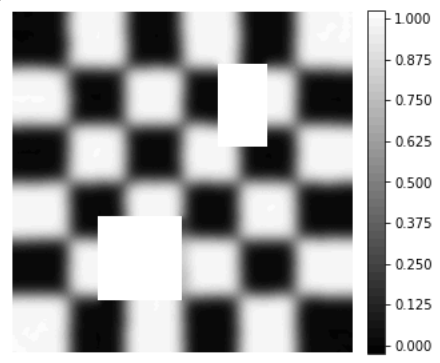
\includegraphics[scale=0.25]{adv_ic_true_tmp.png}
		%		\caption{}
		%		\label{fig:newtoniter2}
	\end{subfigure}
	\begin{subfigure}{0.24\textwidth}
		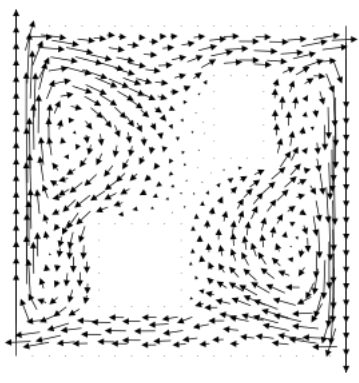
\includegraphics[scale=0.25]{velocity_tmp.png}
		%		\caption{}
		%		\label{fig:newtoniter1}
	\end{subfigure}
	\begin{subfigure}{0.24\textwidth}
		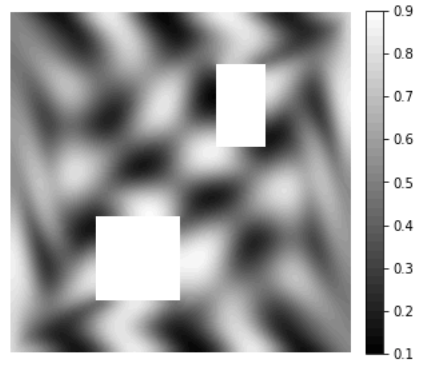
\includegraphics[scale=0.25]{adv_final_condition_true_tmp.png}
		%		\caption{}
		%		\label{fig:newtoniter3}
	\end{subfigure}
	\begin{subfigure}{0.24\textwidth}
		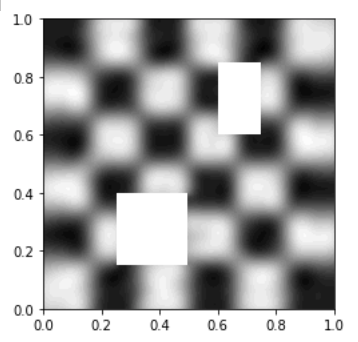
\includegraphics[scale=0.25]{adv_reconstruction_tmp.png}
		%		\caption{}
		%		\label{fig:newtoniter4}
	\end{subfigure}
	%\begin{subfigure}{0.05\textwidth}
	%	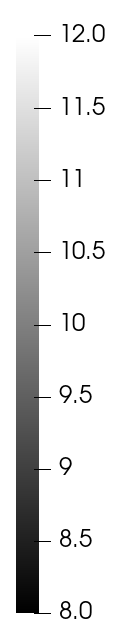
\includegraphics[scale=0.1]{mColorBar.png}
	%\end{subfigure}
	\caption{(a) true initial condition. (b) velocity field. (c) observed concentration at final time. (d) reconstruction of initial condition. black=0, white=1}
	\label{fig:adv_inversion1} 
\end{figure} 


\begin{figure}
	\begin{center}
		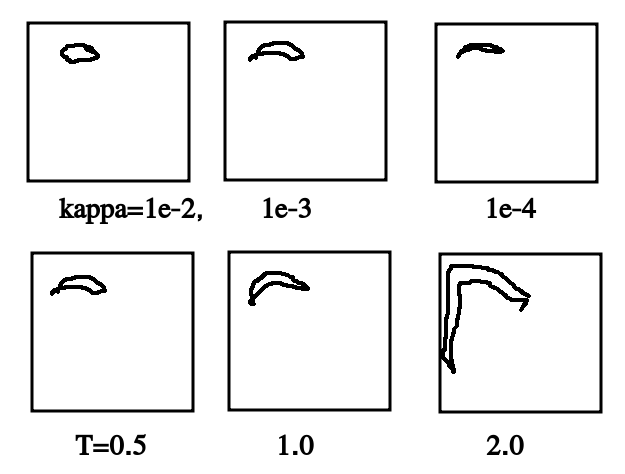
\includegraphics[scale=0.75]{adv_vary_kappa_tf_tmp.png}
	\end{center}
	\caption{Impulse responses for various diffusivities kappa and fixed simulation time Tf=0.5 (top) and simulation times with fixed kappa=1e-3 (bot). Colorbar is normalized independently for each subfigure}
	\label{fig:adv_vary_kappa_tf}
\end{figure}

\begin{figure}
	\begin{subfigure}{0.49\textwidth}
		\centering
		\begin{tikzpicture}[baseline, trim axis right]
		\begin{axis}[width=0.99\linewidth, height=1.0\linewidth,
		ymode=log,
		ymin=1e-11,
		ymax=2,
		xmax=750,
		axis x line*=bottom,
		axis y line*=left,
		xtick={0, 200, 400, 600},
		xlabel={CG iteration},
		ylabel={$||\bm{b}-\bm{H} \bm{x}_k||/||\bm{b}||$},
		title={CG convergence},
		legend style={at={(1.1,1)},anchor=north east},
		%legend pos=north east,
		legend style={font=\small}
		]
		\addlegendentry{Reg}
		\addplot[dotted, line width=0.5mm] table {cg_relres_reg.dat};
		\addlegendentry{None}
		\addplot[dash dot, line width=0.5mm] table {cg_relres_none.dat};
		\addlegendentry{PSF (1)}
		\addplot[blue, line width=0.5mm] table {cg_relres_p1.dat};
		\addlegendentry{PSF (5)}
		\addplot[red, line width=0.5mm] table {cg_relres_p5.dat};
		\addlegendentry{PSF (25)}
		\addplot[purple, line width=0.5mm] table {cg_relres_p25.dat};
		\end{axis}
		\end{tikzpicture}
		\caption{}
		\label{fig:adv_cg_convergence}
	\end{subfigure}
	\begin{subfigure}{0.49\textwidth}
		\centering
		\begin{tikzpicture}[baseline, trim axis right]
		\begin{axis}[width=0.99\linewidth, height=1.0\linewidth,
		xmode=log,
		ymode=log,
		xlabel={$\gamma$, regularization parameter},
		ylabel={\# of CG iterations},
		axis y line*=right,
		axis x line*=bottom,
		ylabel near ticks, yticklabel pos=right,
		%ylabel near ticks, ylabel shift={-6pt},
		%legend pos=north east,
		title={Regularization robustness}
		%title={CG iterations to achieve $||H x-b||/||b||<10^{-6}$}
		]
		%\addlegendentry{None}
		\addplot[dash dot, line width=0.5mm] table[x=gamma, y=none] {CGitsvsGamma.dat};
		%\addlegendentry{REG}
		\addplot[dotted, line width=0.5mm] table[x=gamma, y=reg] {CGitsvsGamma.dat};
		%\addlegendentry{PSF (1)}
		\addplot[blue, line width=0.5mm] table[x=gamma, y=psf1] {CGitsvsGamma.dat};
		%\addlegendentry{PSF (5)}
		\addplot[red, line width=0.5mm] table[x=gamma, y=psf5] {CGitsvsGamma.dat};
		%\addlegendentry{PSF (25)}
		\addplot[purple, line width=0.5mm] table[x=gamma, y=psf25] {CGitsvsGamma.dat};
		\end{axis}
		\end{tikzpicture}
		\caption{}
		\label{fig:adv_kappa_sweep}
	\end{subfigure}
	\caption{Left (\ref{fig:adv_cg_convergence}) shows the convergence history for solving $\bm{H} \bm{x} = \bm{b}$ using PCG, where $\bm{b}$ has i.i.d. random entries drawn from the standard normal distribution. BLAH BLAH BLAH
		%		The y-axis is $||b-Hx_k||/||b||$, where $x_k$ is the $k$th PCG iterate. 
		Here we use $\gamma=9999 \times 10^9$, which is determined by the Morozov discrepancy principle. Right (\ref{fig:adv_kappa_sweep}) shows the number of PCG iterations required to achieve $||\bm{b}-\bm{H} \bm{x}_k||/||\bm{b}|| < 10^{-6}$, where $\bm{x}_k$ is the $k$th PCG iterate, for a range of different $\kappa$. Results in these figures are shown for our preconditioner with 5, 15, and 30 batches (PSF (5), PSF (15), and PSF(30), respectively), regularization preconditioning (REG), and no preconditioning (NONE). The preconditioner is constructed using $\bm{H}_\text{gn}$.}
	\label{fig:adv_krylov_convergence}
\end{figure} 

\begin{figure}
	\begin{subfigure}{0.59\textwidth}
		\begin{center}
			\begin{tikzpicture}[baseline, trim axis right]
			\begin{axis}[width=0.99\linewidth, height=0.8\linewidth,
			ymode=log,
			xmin=-50,
			xmax=1450,
			ymax=1.e4,
			xlabel={$k$, generalized eigenvalue \#},
			ylabel={$\lambda_{k}$},
			xtick={0, 300, 600, 900, 1200},
			%legend pos=north east,
			legend style={font=\small},
			ylabel near ticks, ylabel shift={-6pt},
			axis x line*=bottom,
			axis y line*=left,
			legend style={at={(0.95,1)},anchor=north east},
			title={Generalized eigenvalues, $\bm{H} \genericvec_{k}=\lambda_{k} \bm{\preconditioner} \genericvec_{k}$}
			]
			\addlegendentry{REG}
			\addplot[dotted, line width=0.5mm] table[x=k, y=reg] {generalizedEigenvalues.dat};
			\addlegendentry{PSF (1)}
			\addplot[blue, line width=0.5mm] table[x=k, y=psf1] {generalizedEigenvalues.dat};
			\addlegendentry{PSF (5)}
			\addplot[red, line width=0.5mm] table[x=k, y=psf5] {generalizedEigenvalues.dat};
			\addlegendentry{PSF (25)}
			\addplot[purple, line width=0.5mm] table[x=k, y=psf25] {generalizedEigenvalues.dat};
			\end{axis}
			\end{tikzpicture}
		\end{center}
		\caption{}
		\label{fig:adv_generalized_eigenvalues}
	\end{subfigure}
	\begin{subfigure}{0.39\textwidth}
		\begin{center}
			\begingroup
			\setlength{\tabcolsep}{4pt}
			\renewcommand{\arraystretch}{1.25}
			\begin{tabular}{c| c c}
				& $\kappa(\bm{\preconditioner}^{-1} \bm{H})$\\
				\hline 
				REG        & 7.02e+3 \\
				NONE       & 8.71e+2 \\
				PSF $(5)$  & 1.75e+1 \\
				PSF $(15)$  & 1.39e+1 \\
				PSF $(30)$ & 1.03e+1
			\end{tabular}
			\endgroup
		\end{center}
		\caption{}
		\label{fig:adv_condition_number}
	\end{subfigure}
	\caption{Left (\ref{fig:adv_generalized_eigenvalues}): eigenvalues for generalized eigenvalue problem $\bm{H} \bm{u}_k = \lambda_k \bm{\preconditioner} \bm{u}_k$. Here $\bm{H}$ is the Hessian and $\bm{\preconditioner}$ is the PSF approximation constructed using the Gauss-Newton Hessian, $\bm{H}_\text{gn}$, for 5, 15, and 30 batches (PSF (5), PSF (15), and PSF (30), respectively), or the regularization Hessian (REG). Right (\ref{fig:adv_condition_number}): condition number for $\bm{\preconditioner}^{-1} \bm{H}$ and $\bm{\preconditioner}^{-1} \bm{H}_\text{gn}$ for these different preconditioners, and no preconditioner (NONE). COND(H) LABELS!}
	\label{fig:adv_spectrum}
\end{figure}

\begin{itemize}
	\item Picture of velocity field, initial condition, final condition, reconstruction (1) (OKOK)
	\item Impulse responses: vary time and Peclet number (3) (OKOK)
	\item CG convergence (1) CG iters vs Peclet number (Morozov) (2) (OKOK)
	\item Preconditioned spectrum, condition numbers? (1)
\end{itemize}


\section{Conclusions}
\label{sec:conclusions}

We presented an efficient matrix-free PSF method for approximating operators with locally supported non-negative integral kernels. The method only requires access to the operator via application of the operator to a small number of vectors. The idea of the method is to compute batches of impulse responses by applying the operator to Dirac combs of scattered point sources, then interpolate these impulse responses to approximate entries of the operator's integral kernel. The interpolation is based on a new principle we call ``local mean displacement invariance,'' which generalizes and improves upon classical local translation invariance. The ability to quickly approximate arbitrary integral kernel entries permits us to form an H-matrix approximation of the operator. Fast H-matrix arithmetic is then used to perform further linear algebra operations that cannot be performed easily with the original operator, such as matrix factorization and inversion. The supports of the impulse responses are estimated to be contained in ellipsoids, which are determined a-priori via a new procedure that involves applying the operator to a small number of polynomial functions. Point source locations for the impulse response batches are chosen using a greedy ellipsoid packing procedure, in which we choose as many impulse responses per batch as possible, while ensuring that the corresponding ellipsoids do not overlap. We applied the method to approximate the Gauss-Newton Hessian in a Stokes ice sheet inverse problem, and saw that the approximation substantially outperforms existing Hessian approximation methods. Although the method we presented is not applicable to all Hessians, it is applicable to many Hessians of practical interest. For these Hessians, our method offers a \emph{data scalable} alternative to conventional low rank approximation, because our method can form high rank approximations of an operator using a small number of operator applies, and thus forward and adjoint PDE solves.

\appendix


%\section{Hierarchical matrix details}
%\label{app:h_matrix}
%
%Often, large dense matrices of practical interest may be permuted, then partitioned into blocks recursively, in such a way that many off-diagonal blocks of the matrix are numerically low rank, even if the matrix is high rank. Such matrices are known as hierarchical matrices (H-matrices). Many classes of H-matrices exist (H1, H2, HSS, HBS, and more), and all of these types of H-matrices could be used in conjunction with our product-convolution approximation. Here we use classical H1 matrices. For this section, when we say H-matrix, we are referring to H1 matrices. 
%
%While a dense $\fedim \times \fedim$ matrix traditionally requires $O(\fedim^2)$ memory to store, H-matrices may be stored using $O(\fedim \log \fedim)$ memory, by storing only the low rank factors for the low rank blocks. Recursive algorithms can take advantage of the H-matrix low rank block structure to perform matrix arithmetic fast. Conventional dense matrix algorithms for matrix inversion, matrix factorization, matrix-vector products, matrix-matrix products, and matrix-matrix addition require either $O(\fedim^2)$ or $O(\fedim^3)$ time and memory, while the aforementioned recursive algorithms can perform these matrix operations in $O(\fedim \log(\fedim)^a)$ time and memory for H-matrices. Here $a=0, 1, 2$, or $3$ depending on the operation and type of H-matrix. For more details on H-matrices, we recommend~\cite{HMATRIXGOOD}. 
%
%
%\subsection{H-matrix construction}
%\label{sec:H_matrix_construction}
%
%The process of constructing an H-matrix representation of $\mathbf{\Aker}$ proceeds as follows. First, we construct hierarchical partitionings of the degrees of freedom for the columns and rows of the matrix (cluster trees, Section~\ref{sec:cluster_trees}). Second, we construct a hierarchical partitioning of the blocks of the matrix, in such a way that many of the blocks in the partitioning are expected to be low rank, and the remaining high rank blocks are small (block cluster tree, Section~\ref{sec:block_cluster_tree}). Finally, we form low rank approximations of the blocks of the matrix that are expected to be low rank (adaptive cross approximation, Section~\ref{sec:adaptive_cross}), and fill in the remaining high rank  blocks with their numerical values. The first two steps require geometric information about the spatial locations of the degrees of freedom associated with the rows and columns of the matrix, but these steps do not depend on the particular values of matrix entries. The third step requires us to evaluate $O(\fedim \log \fedim)$ specially-chosen entries of $\mathbf{\Aker}$, and we evaluate these entries using~\eqref{eq:Akerpcmat_entries}. 
%
%
%\subsubsection{Cluster trees}
%\label{sec:cluster_trees}
%
%We use recursive hyperplane splitting to hierarchically cluster the degrees of freedom associated with the columns and rows of the matrix into a \emph{column cluster tree} and a \emph{row cluster tree}, respectively. Here we describe construction of the column cluster tree; the row cluster tree is constructed similarly. 
%
%Since we use finite elements to discretize the problem, the $i^\text{th}$ column of $\mathbf{\Aker}$ corresponds to the Lagrange node in $\mathbb{R}^\gdim$ associated with the $i\text{th}$ finite element basis function. The columns of the matrix thus correspond to a point cloud in $\mathbb{R}^\gdim$. We split this point cloud into two equally sized \emph{child} point clouds, using a hyperplane which is perpendicular to the coordinate axis direction in which the point cloud is widest (e.g., either the $x$, $y$, or $z$ axis in $3$D). The two child point clouds are split in the same way. This splitting process repeats until the point clouds have less than a preset number of points (we use $32$ points). This hierarchical partitioning of the point cloud into smaller and smaller point clouds corresponds to a hierarchical partitioning of the columns of the matrix into smaller and smaller \emph{clusters} of columns. This hierarchical partitioning of the columns forms a binary tree, which is called the column cluster tree. The root of the tree is the set of all columns, and the leaves of the tree are clusters of columns that are not subdivided any further. 
%
%A depth-first search ordering of the column cluster tree leaves is then generated. When the columns of the matrix are permuted into this depth-first ordering, the columns associated with each cluster in the cluster tree are contiguous.
%
%In the same way, the degrees of freedom associated with the rows of the matrix are hierarchically clustered into another cluster tree, and a depth-first search ordering for the rows is generated. In our examples, the degrees of freedom for the columns coincide with the degrees of freedom for the rows, so the cluster trees for the rows and columns are the same, but this is not required in general.
%
%
%\subsubsection{Block cluster tree} 
%\label{sec:block_cluster_tree}
%
%We partition the matrix into a recursive hierarchy of mostly low rank blocks called the \emph{block cluster tree}. The idea is that a block of the matrix is likely to be low rank if the point cloud associated with the rows of the block is far away from the point cloud associated with the columns of the block. This is reasonable to expect here because of the locality property of $\Aop$. Indeed, locality implies that many blocks of the matrix corresponding to far away point cloud clusters will be rank zero.
%
%After reordering the rows and columns of $\mathbf{\Aker}$ via the depth-first ordering described above, we partition the reordered version of $\mathbf{\Aker}$ into a tree of $2 \times 2$ block matrices recursively. We use a geometric admissibility condition (discussed below) to decide which blocks to subdivide, and use the cluster trees for the rows and columns to determine how to subdivide those blocks. For the first stage of subdivision, let $r_1$ and $r_2$ be the children row clusters for the root of the row cluster tree, let $\colcluster_1$ and $\colcluster_2$ be the children column clusters for the root of the column cluster tree. The matrix $\mathbf{\Aker}$ is partitioned into blocks as follows:
%\begin{equation*}
%	\begin{bmatrix}
%		\mathbf{\Aker}_{11} & \mathbf{\Aker}_{12} \\
%		\mathbf{\Aker}_{21} & \mathbf{\Aker}_{22}
%	\end{bmatrix},
%\end{equation*}
%where $\mathbf{\Aker}_{11}$ denotes the block of $\mathbf{\Aker}$ with rows $r_1$ and columns $\colcluster_1$, $\mathbf{\Aker}_{12}$ denotes the block of $\mathbf{\Aker}$ with rows $r_1$ and columns $\colcluster_2$, and so on for $\mathbf{\Aker}_{21}$ and $\mathbf{\Aker}_{22}$.
%
%We now loop through the four blocks, $\mathbf{\Aker}_{11}$, $\mathbf{\Aker}_{12}$, $\mathbf{\Aker}_{21}$, and $\mathbf{\Aker}_{22}$, and decide which blocks should be subdivided further. For the purpose of explanation, consider $\mathbf{\Aker}_{12}$. If
%\begin{equation}
%	\label{eq:weak_admissibility_cond}
%	\dist\left(r_1, \colcluster_2\right) \ge \weakadmconst \min\left(\diam\left(r_1\right), \diam\left(\colcluster_2\right)\right),
%\end{equation}
%then we mark $\mathbf{\Aker}_{12}$ as \emph{admissible} (expected to be low rank) and leave it alone. Here $\dist\left(r_1, \colcluster_2\right)$ is the Euclidean distance between the axis-aligned bounding box for the point cloud associated with the row cluster $r_1$, and the axis aligned bounding box for the point cloud associated with the column cluster $\colcluster_2$. The quantity $\diam\left(r_1\right)$ is the diameter of the axis aligned bounding box for the point cloud associated with the row cluster $r_1$, and $\diam\left(\colcluster_2\right)$ is the analogous diameter associated with the column cluster $\colcluster_2$. Here the quantity $\weakadmconst$ is a scalar constant; we use $\weakadmconst=2.0$. Basically, if the point clouds associated with $r_1$ and $\colcluster_2$ are far away from each other relative to their diameters, then we expect that the corresponding block of the matrix will be low rank. This process is repeated for the other blocks to determine which blocks are admissible and which are not. For us, the diagonal blocks $\mathbf{\Aker}_{11}$ and $\mathbf{\Aker}_{22}$ are not admissible because the distance between a point cloud and itself is zero. 
%
%Next, we subdivide all blocks that are not admissible and are larger than a predetermined size (we use size $32 \times 32$), using the same process that was used to subdivide $\mathbf{\Aker}$. But now we subdivide a block based on the two child row clusters and two child column clusters for the rows and columns of that block. This subdivision process continues recursively until all blocks are either admissible, or smaller than the predetermined size mentioned above. The resulting hierarchical partitioning of matrix blocks forms a tree, which is called the \emph{block cluster tree}. The root of the tree is the whole matrix, internal nodes in the tree are blocks that are subdivided, and the leaves of the tree are blocks that are either expected to be low rank, or are small.
%
%
%\subsubsection{Adaptive cross low rank approximation of blocks}
%\label{sec:adaptive_cross}
%
%Once the block cluster tree has been constructed, low rank approximations of the admissible (low rank) blocks are formed using the adaptive cross method~\cite{ACA}. Let $X \in \mathbb{R}^{m \times m}$ be an admissible block of $\mathbf{\Aker}$. The idea of the adaptive cross method is to form a low rank approximation of $X$ by sampling a small number of rows and columns of $X$. 
%\begin{itemize}
%	\item Let $C \in \mathbb{R}^{m \times \hrank}$ be a matrix consisting of a subset of $\hrank$ columns of $X$, such that the span of the columns in $C$ approximates the column space of $X$. 
%	\item Let $R\in\mathbb{R}^{\hrank \times m}$ be a subset of the rows of $X$, such that the span of the rows in $R$ approximates the row space of $X$.
%	\item Let $U \in \mathbb{R}^{\hrank \times \hrank}$ be the block of $X$ consisting of the intersection of the rows from $R$ with the columns from $C$.
%\end{itemize}
%Then it is well-established that
%\begin{equation}
%	\label{eq:CUR}
%	X \approx C U^+ R,
%\end{equation}
%where $U^+$ is the pseudoinverse of $U$~\cite{goreinov1997theory,MahoneyDrineas09}. The quality of approximation~\eqref{eq:CUR} depends on how well the columns of $C$ approximate the column space of $X$, and how well the rows of $R$ approximate the row space of $X$. 
%
%In the adaptive cross method, ``good'' columns, $C$, and rows, $R$, are chosen via an alternating iterative process. An initial set of columns $C$ is chosen. Keeping $C$ fixed, a set of rows $R$ is chosen so that the so that determinant of the submatrix $U$ within $C$ is as large as possible~\cite{GoreinovEtAl10}. Now, keeping $R$ fixed, a set of new columns $C$ is chosen so that the submatrix $U$ within $R$ is as large as possible. This process repeats a small number of times. This results in matrices $R$ and $C$ such that the error in the approximation,~\eqref{eq:CUR}, is small. The dominant cost of this procedure is the cost of computing $a \hrank$ columns of $X$ and $a\hrank$ rows of $X$, where $a$ is the number of alternating iterations. There is also a small linear algebra overhead cost for the determinant maximization process that is performed at each step. 
%The key point is that the adaptive cross method allows us to form a rank-$\hrank$ approximation of an $m \times m$ block of the matrix via a process that only requires accessing $O(m\hrank)$ entries of that block.
%
%We use the adaptive cross method to form low rank approximations for each admissible block of $\mathbf{\Aker}$. We directly compute all entries of the small dense blocks of $\mathbf{\Aker}$ that are not admissible. This process requires us to compute $O(\hrank^2 \fedim \log \fedim)$ entries of $\mathbf{\Aker}$, which is relatively cheap compared to the operator actions of $\Aop$ that are required to form the product-convolution approximation.


\section{Ellipsoid intersection test}
\label{sec:fast_ellipsoid_intersection_test}
The procedure for choosing sample points relies on quickly determining whether two ellipsoids intersect. Let $E_1$ and $E_2$ be the ellipsoids defined as
\begin{align*}
	E_i :=& \{x : (x - \spatialmean_i)^T \spatialcov_i^{-1} (x - \spatialmean_i) \le \tau^2\}
\end{align*}
for $i\in\{1,2\}$, where $\spatialmean_1, \spatialmean_2 \in \mathbb{R}^\gdim$, and $\spatialcov_1, \spatialcov_2 \in \mathbb{R}^{\gdim \times \gdim}$ are positive definite. Let $K$ be the following one dimensional convex function:
\begin{equation*}
	K(s) := 1 - \frac{1}{\tau^2} (\spatialmean_1 - \spatialmean_2)^T \left(\frac{1}{1-s}\spatialcov_1 + \frac{1}{s}\spatialcov_2\right)^{-1}(\spatialmean_1 - \spatialmean_2).
\end{equation*}
In~\cite{GilitschenskiHanebeck12} it is shown that $E_1 \cap E_2 = \{\}$ if and only if $K(s) < 0$ for some $s\in (0,1)$.
% (see Figure~\ref{fig:ellipsoid_intersection_test}). 

%\begin{figure}
%	\begin{subfigure}{0.37\textwidth}
%		\centering
%		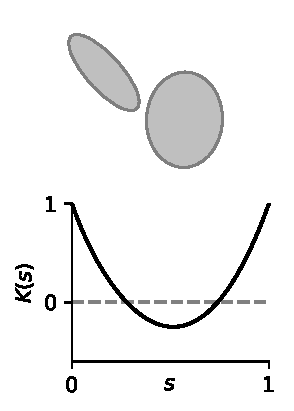
\includegraphics[scale=1.0]{ellipsoids_intersect0.pdf}
%	\end{subfigure}
%	\begin{subfigure}{0.30\textwidth}
%		\centering
%		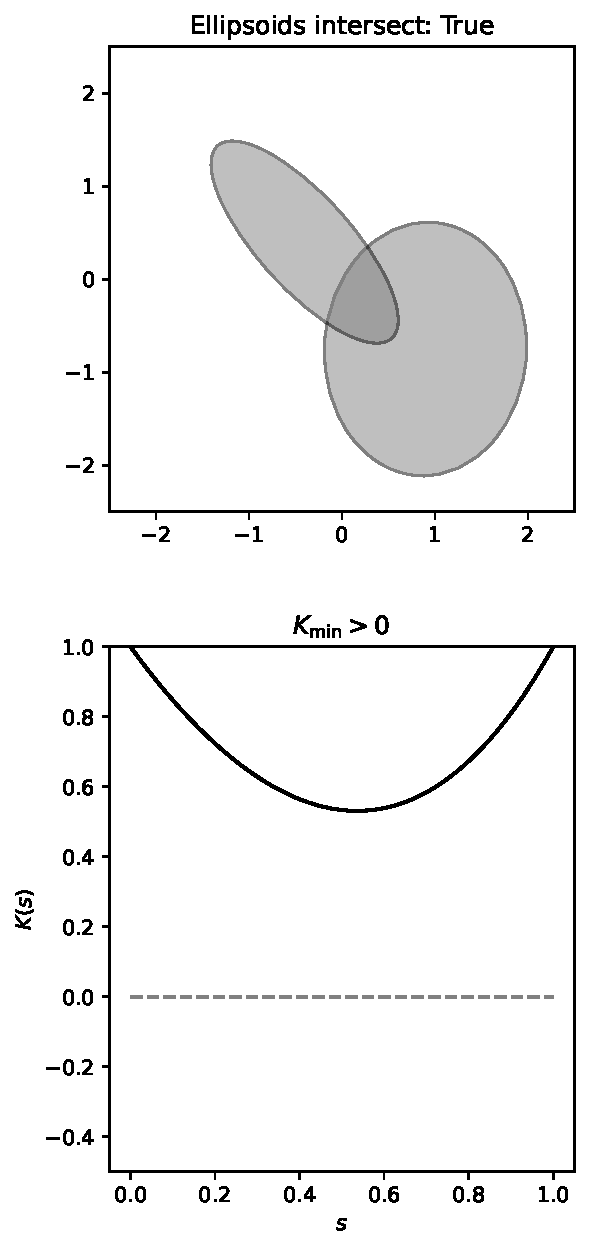
\includegraphics[scale=1.0]{ellipsoids_intersect1.pdf}
%	\end{subfigure}
%	\begin{subfigure}{0.30\textwidth}
%		\centering
%		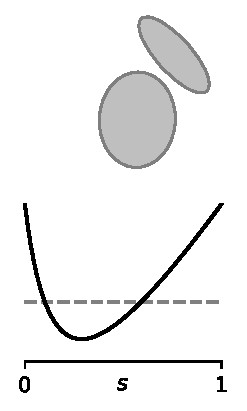
\includegraphics[scale=1.0]{ellipsoids_intersect2.pdf}
%	\end{subfigure}
%	\caption{The ellipsoids intersect if $K(s) \ge 0$ for all $s \in (0,1)$.
%	}
%	\label{fig:ellipsoid_intersection_test}
%\end{figure}

The function $K(s)$ may be evaluated quickly for many $s$ by computing the solution to the generalized eigenvalue problem
$
	\spatialcov_1 \eigenvectormatrix = \spatialcov_2 \eigenvectormatrix \Lambda,
$
where $\eigenvectormatrix \in \mathbb{R}^{\gdim \times \gdim}$ is the matrix of generalized eigenvectors, and $\Lambda = \diag(\lambda_1,\lambda_2,\dots,\lambda_\gdim)$ is the diagonal matrix of generalized eigenvalues $\lambda_i$. 
%The matrix $\eigenvectormatrix$ simultaneously diagonalizes $\spatialcov_1$ and $\spatialcov_2$, in the sense that $\eigenvectormatrix^T\spatialcov_1 \eigenvectormatrix = \Lambda$, and $\eigenvectormatrix^T\spatialcov_2 \eigenvectormatrix = I$, where $I$ is the $\gdim \times \gdim$ identity matrix. Using this diagonalization, and 
After some algebraic manipulations, we have
\begin{equation}
	\label{eq:Ks_generalized}
	K(s) = 1 - \frac{1}{\tau^2} \sum_{i=1}^\gdim \frac{s(1-s)}{1 + s (\lambda_i - 1)}v_i^2,
\end{equation}
where $v := \eigenvectormatrix^T\left(\spatialmean_1 - \spatialmean_2\right)$. To check whether $E_1$ and $E_2$ intersect, we compute the generalized eigenvalue decomposition of $\spatialcov_1$ and $\spatialcov_2$, form $v$, then minimize $K(s)$ in the form~\eqref{eq:Ks_generalized} on $(0,1)$ using Brent's method~\cite{Brent71}. If $K(s^*) <0$ at the minimizer, $s^*$, then $E_1 \cap E_2 = \{\}$. Otherwise $E_1 \cap E_2 \neq \{\}$.
%The resulting algorithm for checking whether $E_1$ and $E_2$ intersect is summarized in Algorithm~\ref{alg:ellipsoid_intersection_test}.

%\begin{algorithm2e}
%	\SetAlgoNoLine
%	\SetKwInOut{Input}{Input}
%	\SetKwInOut{Output}{Output}
%	\SetKwProg{Fn}{Function}{}{}
%	\Input{Ellipsoid $E_1$ with mean $\spatialmean_1$ and covariance $\spatialcov_1/\tau^2$\\
%		Ellipsoid $E_2$ with mean $\spatialmean_2$ and covariance $\spatialcov_2/\tau^2$ 
%	}
%	
%	\Output{Boolean $\text{ellipsoids\_intersect}$ which is true if $E_1 \cap E_2 \neq \{\}$ and false otherwise}
%	
%	
%	Solve generalized eigenvalue problem $\spatialcov_1 P = \spatialcov_2 P \Lambda$
%		
%	$v \gets P^T\left(\spatialmean_1 - \spatialmean_2\right)$
%		
%	$\displaystyle K^* \gets \min_{s \in (0,1)}~1 - \frac{1}{\tau^2} \sum_{i=1}^\gdim \frac{s(1-s)}{1 + s (\lambda_i - 1)}v_i^2$
%		
%	\If{$K^* < 0$}{
%			
%		$\text{ellipsoids\_intersect} \gets \text{False}$
%			
%	}
%	\Else{
%			
%		$\text{ellipsoids\_intersect} \gets \text{True}$
%			
%	}
%	\caption{Determining whether two ellipsoids intersect}
%	\label{alg:ellipsoid_intersection_test}
%\end{algorithm2e}

%\subsection{Ellipsoid bounding box test}

This ellipsoid intersection test is only performed if the coordinate axis aligned bounding boxes for the ellipsoids intersect. The smallest coordinate axis aligned box that contains $E_i$ is the box
$
	\prod_{k=1}^\gdim \left[ \spatialmean_i^{k} -\tau\sqrt{\Sigma_i^{kk}}, \spatialmean_i^{k} +\tau\sqrt{\Sigma_i^{kk}} \right],
$
where $\spatialmean_i^{k}$ is the $k$th entry of $\spatialmean_i$, and $\Sigma_i^{kk}$ is the $k$th diagonal entry of $\Sigma_i$\footnote{See \url{https://math.stackexchange.com/q/3928964}}. The boxes
$\prod_{k=1}^\gdim \left[a_{-}^k, a_{+}^k\right]$ and $\prod_{k=1}^\gdim \left[b_{-}^k, b_{+}^k\right]$
intersect if and only if $a_{-}^k \le b_{+}^k$ and $b_{-}^k \le a_{+}^k$ for $k=1,\dots,d$.




\section{Rational positive semi-definite modification}
\label{sec:make_spd}
In many problems $\Aop$ is symmetric positive semi-definite. However, $\mathbf{A}_H$ is non-symmetric and indefinite because of approximation error. 
This is undesirable. Symmetry and positive semi-definiteness are important properties which should be preserved if possible. Also, lacking these properties may prevent one from using highly effective algorithms, such as the conjugate gradient method, to perform further operations involving $\mathbf{A}_H$. 

If $\Aop$ is symmetric, we symmetrize $\mathbf{A}_H$ as follows:
$
\mathbf{A}_H^{\text{sym}} := \frac{1}{2}\left(\mathbf{A}_H + \mathbf{A}_H^T\right).
$
If $\Aop$ is positive semi-definite, we adapt the rational method from~\cite[Section 13.8]{HackbuschKress07} to approximate the matrix absolute value of $\mathbf{A}_H^{\text{sym}}$, which we denote by $|\mathbf{A}_H^{\text{sym}}|$. That is, $|\mathbf{A}_H^{\text{sym}}|$ has the same eigenvectors as $\mathbf{A}_H^{\text{sym}}$, but the eigenvalues of $|\mathbf{A}_H^{\text{sym}}|$ are the absolute values of the eigenvalues of $\mathbf{A}_H^{\text{sym}}$.
%flip (or approximately flip) the negative eigenvalues of $\mathbf{A}_H^{\text{sym}}$ to be positive. 
Once constructed, we use the approximation of $|\mathbf{A}_H^{\text{sym}}|$ in place of $\mathbf{A}_H$ in further linear algebra operations.

In detail, let $a$ be any scalar satisfying $-a < \lambda_\text{min}$, where $\lambda_\text{min}$ is the smallest eigenvalue of $\mathbf{A}_H^{\text{sym}}$, and set 
\begin{equation}
\label{eq:ratT999}
\mathbf{T} :=  \left(2 \mathbf{A}_H^{\text{sym}} + a \mathbf{I}\right)/a,
\end{equation}
From the results in~\cite[Section 13.8]{HackbuschKress07} it is straightforward to show that
\begin{equation}
\label{eq:rational343}
\mathbf{\Pi}_\ratord := \left(\mathbf{I} + \mathbf{T}^{2^\ratord}\right)^{-1}
\end{equation}
approximates the spectral projector onto the eigenspace of $\mathbf{A}_H^{\text{sym}}$ corresponding to negative eigenvalues. Thus, we have
\begin{equation}
\label{eq:rational76567}
|\mathbf{A}_H^{\text{sym}}| \approx \left(\mathbf{I} - 2\mathbf{\Pi}_\ratord\right)\mathbf{A}_H^{\text{sym}}.
\end{equation}
To form an approximation of $|\mathbf{A}_H^{\text{sym}}|$, first, we compute $\lambda_\text{min}$ using the Lanczos method, and set $a=\gamma \lambda_\text{min}$, where $\gamma\ge 1$ is a parameter that must be chosen. 
The method is relatively insensitive to $\gamma$ and numerically we find that the method works well for any $\gamma \in [1,2]$. We use $\gamma=1.5$ in our numerical results. 
Next, we compute $\mathbf{T}$ per~\eqref{eq:ratT999}, compute $\mathbf{T}^{2^\ratord}$ per~\eqref{eq:rational343} via repeated squaring, compute $\mathbf{\Pi}_\ratord$ per~\eqref{eq:rational343}, and form an approximation of $|\mathbf{A}_H^{\text{sym}}|$ per~\eqref{eq:rational76567}. Fast H-matrix methods are used to perform the required matrix-matrix additions and multiplications, and matrix inversion. We recommend using $\ratord=1$ or $2$. Larger $\ratord$ is unnecessary and may make the method unstable. 

%Finally, we approximate $|\mathbf{A}_H^{\text{sym}}|$ per~\eqref{eq:rational76567}, using fast H-matrix operations to perform the required matrix-matrix addition and matrix inversion.

%
%define $
%\mathbf{T} := T(\mathbf{A}_H^{\text{sym}}) = \left(2 \mathbf{A}_H^{\text{sym}} + a \mathbf{I}\right)/a.
%$, where $-a < \lambda_\text{min}$, where $\lambda_\text{min}$ is the smallest eigenvalue of $\mathbf{A}_H^{\text{sym}}$ and define
%
%let $\mathbf{\Pi}$ be the spectral projector onto the eigenspace of $\mathbf{A}_H^{\text{sym}}$ corresponding to eigenvalues of $\mathbf{A}_H^{\text{sym}}$ that reside in $(-a,0)$
%% let $\Pi$ be the indicator function for the interval $(a,b)$. 
%%That is, $\Pi(\lambda)=0$ for $\lambda \in (0,1)$, and $\Pi(\lambda)=0$ otherwise.
%%\begin{equation*}
%%	\Pi(\lambda) = \begin{cases}
%%		1, & \lambda \in (a,b), \\
%%		0, & \text{otherwise}.
%%	\end{cases}
%%\end{equation*}
%%Using functional calculus to extend the domain of the function $\Pi$ from scalars to matrices, we define
%%$
%%\mathbf{\Pi} := \Pi(\mathbf{A}_H^{\text{sym}}).
%%$
%%The matrix $\mathbf{\Pi}$ is the spectral projector onto the eigenspace of $\mathbf{A}_H^{\text{sym}}$ corresponding to eigenvalues of $\mathbf{A}_H^{\text{sym}}$ that reside in $(a,b)$. 
%If we choose $-a < \lambda_\text{min}$, where $\lambda_\text{min}$ is the smallest eigenvalue of $\mathbf{A}_H^{\text{sym}}$, then $\mathbf{\Pi}$ is the spectral projector onto the eigenspace associated with negative eigenvalues, 
%%and $\mathbf{\Pi}\mathbf{A}_H^{\text{sym}}$ is the ``negative component'' of $\mathbf{A}_H^{\text{sym}}$ in which all the negative eigenvalues are the same but all the positive eigenvalues are replaced by zero. Subtracting a negative number from itself twice flips its sign,
%so the matrix absolute value of $\mathbf{A}_H^{\text{sym}}$ is given by
%\begin{equation}
%\label{eq:I_Pi_abs}
%	|\mathbf{A}_H^{\text{sym}}| = \left(\mathbf{I} - 2\mathbf{\Pi}\right)\mathbf{A}_H^{\text{sym}},
%\end{equation}
%where $\mathbf{I}$ is the identity matrix of the appropriate size.
%By ``matrix absolute value,'' we mean that $|\mathbf{A}_H^{\text{sym}}|$ is the matrix that has the same eigenvectors as $\mathbf{A}_H^{\text{sym}}$, but the eigenvalues of $|\mathbf{A}_H^{\text{sym}}|$ are the absolute values of the eigenvalues of $\mathbf{A}_H^{\text{sym}}$.
%%\begin{figure}
%%	\centering
%%	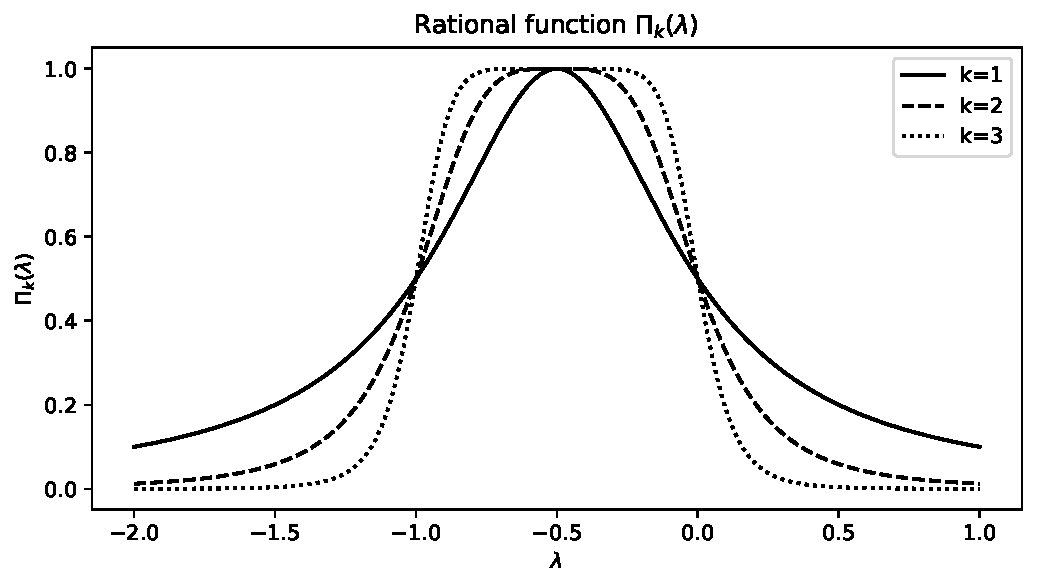
\includegraphics[scale=0.5]{spd_rational_function.pdf}
%%	\caption{Rational function $\Pi_\ratord(\lambda)$ for $a=-1$, $b=0$, and $\ratord \in \{1,2,3\}$. As $\ratord$ increases, $\Pi_\ratord$ approaches the indicator function for the set $(a,b)$. }
%%	\label{fig:spd_rat}
%%\end{figure}
%Computing $\mathbf{\Pi}$ directly is difficult, but we may approximate $\mathbf{\Pi}$ by the following high order rational matrix function,
%%$\Pi_\ratord \approx \Pi$ which is defined as follows:
%%\begin{equation*}
%%	 \Pi_\ratord(\lambda) := \frac{1}{1 + T(\lambda)^{2^\ratord} }, \qquad \text{where} \qquad T(\lambda) := \frac{2 \lambda - (b+a)}{b-a}.
%%\end{equation*}
%%Here $\ratord$ is a positive integer; the larger $\ratord$ is, the better the approximation $\Pi \approx \Pi_\ratord$. 
%%%This is illustrated in Figure~\ref{fig:spd_rat}. 
%%Replacing scalar operations with matrix operations, we have an approximation $\mathbf{\Pi}_\ratord \approx \mathbf{\Pi}$ given by
%\begin{equation}
%\label{eq:rational343}
%\mathbf{\Pi} \approx \mathbf{\Pi}_\ratord := \left(\mathbf{I} + \mathbf{T}^{2^\ratord}\right)^{-1},
%\end{equation}
%where
%$
%\mathbf{T} := T(\mathbf{A}_H^{\text{sym}}) = \left(2 \mathbf{A}_H^{\text{sym}} + a \mathbf{I}\right)/a.
%$
%Using $\mathbf{\Pi}_\ratord$ instead of $\mathbf{\Pi}$ in~\eqref{eq:I_Pi_abs} allows us to approximate $|\mathbf{A}_H^{\text{sym}}|$. First, we compute $\lambda_\text{min}$ using the Lanczos method, and set $a=\gamma \lambda_\text{min}$ and $b=0$, where $\gamma\ge 1$ is a parameter that must be chosen. 
%The method is relatively insensitive to $\gamma$ and numerically we find that the method works well for any $\gamma \in [1,2]$. We use $\gamma=1.5$ in our numerical results. 
%Next, we compute $\mathbf{T}$ using fast H-matrix scalar multiplication and addition. We form the $\mathbf{T}^{2^\ratord}$ via repeated squaring using H-matrix multiplication. We recommend using $\ratord=1$ or $2$. Larger $\ratord$ is unnecessary and may make the method unstable. The approximate spectral projector $\mathbf{\Pi}_\ratord$ is formed from $\mathbf{T}^{2^\ratord}$ per~\eqref{eq:rational343}, using fast H-matrix operations to perform the required matrix-matrix addition and matrix inversion. Finally, a positive semi-definite approximation $\mathbf{A}_H^{\text{sym}+}$ of $\mathbf{A}_H^{\text{sym}}$ is formed as
%\begin{equation*}
%\mathbf{A}_H^{\text{sym}+} := \left(\mathbf{I} - 2\mathbf{\Pi}_\ratord\right)\mathbf{A}_H^{\text{sym}},
%\end{equation*}
%where fast H-matrix operations are used to perform the necessary matrix-matrix subtraction and multiplication. Note that for any $\ratord \ge 1$, $\Pi_\ratord(\lambda)> 1/2$ for $\lambda \in (a,b)$, so $\mathbf{A}_H^{\text{sym}+}$ is positive semi-definite\footnote{Some indefiniteness may be introduced by truncation error in the H-matrix operations, but the negative eigenvalues caused by this truncation error are typically extremely small.}. At the end, $\mathbf{A}_H^{\text{sym}+}$ is symmetrized once again, to correct for any small non-symmetries that are introduced by truncation error in the H-matrix operations. Once constructed, we use the symmetric positive semi-definite matrix $\mathbf{A}_H^{\text{sym}+}$ in place of $\mathbf{A}_H$ in further linear algebra operations.

%\section{Recycling Krylov information via low rank updates}
%\label{sec:recycle_krylov}
%
%In applications, often one wants to use the H-matrix approximation $\mathbf{A}_H$ to build preconditioners for solving a sequence of slowly varying linear systems, where the $k$th linear system has the form
%\begin{equation}
%\label{eq:Ax_equals_b}
%\mathbf{B}^{(k)} \mathbf{u}^{(k)} = \mathbf{f}^{(k)}.
%\end{equation}
%Each of these linear systems is solved using an iterative method. By ``slowly varying,'' we mean that $\mathbf{B}^{(k+1)}$ does not differ much from $\mathbf{B}^{(k)}$. 
%For example, in a Newton-Krylov method for solving an optimization problem, one uses a Krylov method such as conjugate gradient to solve a sequence of systems of the form~\eqref{eq:Ax_equals_b}, where $\mathbf{B}^{(k)}$ and $\mathbf{f}^{(k)}$ are the Hessian and the negative gradient of the objective function in the optimization problem, respectively, evaluated at the $k$th Newton iterate. 
%As the optimization solver converges, $\mathbf{B}^{(k)}$ converges to the Hessian at the optimal point, and therefore changes little from one iteration to the next. Since $\mathbf{B}^{(k)}$ varies slowly, it is reasonable to assume that Krylov information about $\mathbf{B}^{(k)}$ can be leveraged to update the preconditioner from $\mathbf{B}^{(k)}$ in order to build a preconditioner for $\mathbf{B}^{(k+1)}$.
%Concretely, let 
%\begin{equation*}
%\mathbf{P}^{(k)} \approx \left(\mathbf{B}^{(k)}\right)^{-1}
%\end{equation*}
%denote a H-matrix preconditioner used to accelerate the solution of~\eqref{eq:Ax_equals_b} with an iterative method. The iterative method for solving the $k$th linear system will typically involve, as a sub-problem, applying $\mathbf{B}^{(k)}$ to a collection of vectors $\{\mathbf{x}_i\}_{i=1}^m$, thereby generating vectors $\{\mathbf{y}_i = \mathbf{B}^{(k)} \mathbf{x}_i\}_{i=1}^m$. Instead of rebuilding the H-matrix preconditioner for each successive linear system, we \emph{recycle} the information generated by the iterative method while solving the current linear system, performing a low-rank update to $\mathbf{P}^{(k)}$ to create $\mathbf{P}^{(k+1)}$. To do so, we build on the rank-1 update formulas discussed in~\cite[Chapter 6]{NocedalWright99}, which we generalize to many vector ``rank-$m$'' updates. In what follows, let $\mathbf{X}$ and $\mathbf{Y}$ denote the $\fedim \times m$ matrices with columns given by the vectors $\mathbf{x}_i$ and $\mathbf{y}_i$, respectively. The matrix-vector products with $\mathbf{B}^{(k)}$ performed while solving the $k$th linear system may be summarized by the equation:
%\begin{equation*}
%\mathbf{B}^{(k)}\mathbf{X} = \mathbf{Y}.
%\end{equation*}
%To form $\mathbf{P}^{(k+1)}$ from $\mathbf{P}^{(k)}$, one may use one of the following three update formulas:
%\begin{align}
%	\mathbf{P}^{(k+1)} &= \mathbf{P}^{(k)} + \mathbf{R}\left(\mathbf{Y}^T \mathbf{Y}\right)^{-1} \mathbf{Y}^T \label{eq:res_update} \\
%	\mathbf{P}^{(k+1)} &= \mathbf{P}^{(k)} + \mathbf{R} \left(\mathbf{R}^T \mathbf{Y}\right)^{-1} \mathbf{R}^T \label{eq:srk_update} \\
%	\mathbf{P}^{(k+1)} &= \left(\mathbf{I} - \mathbf{X}\boldsymbol{\Theta}\mathbf{Y}^T\right)\mathbf{P}^{(k)}\left(\mathbf{I} - \mathbf{Y}\boldsymbol{\Theta}\mathbf{X}^T\right) + \mathbf{X}\boldsymbol{\Theta}\mathbf{X}^T, \label{eq:dfp_update}
%\end{align}
%where $\mathbf{R} := \mathbf{X}-\mathbf{P}^{(k)}\mathbf{Y}$ and $\boldsymbol{\Theta} := \left(\mathbf{X}^T\mathbf{Y}\right)^{-1}$.
%We note that for all three cases, the update is exact for $\mathbf{B}^{k}$, in the sense that 
%\begin{equation*}
%\mathbf{P}^{(k+1)}\mathbf{Y}=\mathbf{X} = \left(\mathbf{B}^{(k)}\right)^{-1} \mathbf{Y}.
%\end{equation*}
%Because the matrices $\mathbf{B}^{k}$ vary slowly, we expect that $\mathbf{P}^{(k+1)}$ is a good approximation for $\left(\mathbf{B}^{(k+1)}\right)^{-1}$ on the space spanned by the vectors $\mathbf{y}_i$. One should choose which formula to use based on the properties of the matrix $\mathbf{B}^{(k)}$. Formula~\eqref{eq:res_update} does not preserve symmetry, and should therefore be used when $\mathbf{B}^{(k)}$ is not symmetric. Formula~\eqref{eq:srk_update} preserves symmetry but not positive definiteness, and should therefore be used when $\mathbf{B}^{(k)}$ is symmetric and indefinite. Formula~\eqref{eq:dfp_update}, which is used in this paper, preserves both symmetry and positive definiteness, and should therefore be used when $\mathbf{B}^{(k)}$ is symmetric positive definite. Formulas~\eqref{eq:res_update} and~\eqref{eq:srk_update} perform rank-$m$ updates, while formula~\eqref{eq:dfp_update} performs a rank-$2m$ update. 
%We note that when $m=1$, formulas~\eqref{eq:srk_update} are~\eqref{eq:dfp_update} are known as SR1 (symmetric rank-$1$) and DFP (Davidson-Fletcher-Powell) updates, respectively~\cite[Chapter 6]{NocedalWright99}. 

\section*{Acknowledgments}
We thank J.J. Alger, Longfei Gao, Mathew Hu, and Rami Nammour for helpful discussions. We thank Trevor Heise for editing suggestions. We thank Georg Stadler for domain geometry help.

\FloatBarrier

\bibliographystyle{siamplain}
\bibliography{localpsf}

\end{document}
